\documentclass[12pt]{article}
\usepackage[utf8]{inputenc}
\usepackage[french]{babel}
\usepackage[tikz]{bclogo}
\usepackage{geometry}
\usepackage{array}
\usepackage{version}
\usepackage{graphics}
\usepackage{graphicx}
\usepackage{pgfgantt}
\usepackage{url}
\usepackage{enumitem}
\usepackage{hyperref}
\bibliographystyle{alpha}
\usepackage[counterclockwise]{rotating}
\geometry{hmargin=2.5cm,vmargin=1.5cm}

\setlength{\parskip}{1ex plus 2ex minus 1ex}
\newcolumntype{M}[1]{
    >{\raggedright}m{#1}
}

\newenvironment{besoins}
{ \begin{itemize}[topsep=20pt]   }
{ \end{itemize}                  } 

\newcommand{\priority}[1] {
  (\textit{Priorité}:#1)
}
\newcommand{\besoin}[3]{
	\item #1 \priority{#2} #3
}

\newcommand{\class}[1]{\texttt{#1}}
\newcommand{\shellcmd}[1]{\\\indent\indent\texttt{\footnotesize\# #1}\\}

\title{
 \begin{minipage}\linewidth
        \centering
        Simulation d'algorithmes d'équilibrage de charge dans un environnement distribué 
        \vskip3pt
        \large Memoire final
    \end{minipage}
 }

\author{Kevin Barreau \and Guillaume Marques \and Corentin Salingue}

\begin{document}

\maketitle

\abstract
Ce document, mémoire final de notre Projet de Programmation, décrit l'ensemble du projet et les algorithmes utilisés. Il contient aussi les besoins fonctionnels et non fonctionnels ainsi que l'architecture du produit final. Enfin, il récapitule point par point le travail effectué ainsi que sa mise en oeuvre. Le document présente les tests effectués et leurs analyses. Enfin, il conclue sur les améliorations possibles du produit.

\newpage


\renewcommand{\contentsname}{Sommaire} 
\tableofcontents

\newpage

\listoffigures

\newpage

\section{Présentation du projet}

Dans le présent document, nous considérons que le lecteur possède des notions en informatique et que chaque mot est défini par son sens commun. Cependant, si un terme qui est utilisé présentant une définition différente que celle admise par tous, nous ne manquerons pas de le préciser et de le définir.

\subsection{Utilisation d'une base de données par un client}

\paragraph{} Une \textit{base de données} est un outil permettant de stocker et récupérer des \textit{données}, qui sont des informations binaires utilisant des structures propres au système de base de données.

\paragraph{} Dans un premier temps, le client se connecte à la base de données.
Le client interagit avec celle-ci en lui envoyant des \textit{requêtes}, messages, dont la forme dépend de la base de données et permettant de stocker, récupérer ou modifier des données.

\paragraph{}Selon les requêtes émises par le client, la base de données lui renvoie des résultats (voir la figure~\ref{fig:bd}).


\begin{figure}[h]
	\centering
		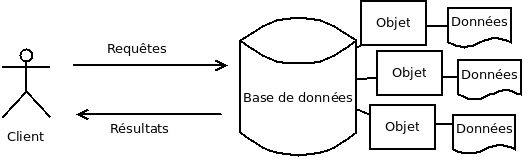
\includegraphics[width=12cm]{images/besoins/bd.png}
	\caption{Interactions client/base de données \label{fig:bd}}
\end{figure}


\paragraph{} On distingue deux types de requêtes :
\begin{itemize}
 \item Les requêtes de \textbf{lecture}: requêtes ne modifiant pas les données contenues dans la base de données.
 Il s'agit de récupérer des objets contenus dans la base de données.
 
 \item Les requêtes d' \textbf{écriture} : requêtes modifiant les données contenues dans la base de données.
\end{itemize}

\paragraph{} Le client peut être une personne physique ou un logiciel. Dans notre cas, il s'agit d'un logiciel permettant l'importation de fichiers contenant des requêtes ou de générer des requêtes pseudo-aléatoirement.


\subsection{Base de données distribuée}

\paragraph{} La base de données utilisée par le client est plus précisément une base de données dite \textit{distribuée}. Le client ne voit pas de différence, lorsqu'il l'utilise, entre une base de données classique et une base de données distribuée. On dit qu'une base de données est distribuée lorsque les données qu'elle stocke sont réparties sur plusieurs machines ou emplacements physiques, appelés \textit{noeuds}. Les noeuds sont capables de communiquer entre eux afin de s'échanger des informations.

\paragraph{} On peut rassembler des noeuds pour former un \textit{data center}. Un rassemblement de data center correspond à un \textit{cluster} (voir la figure~\ref{fig:distributed_database}). Dans ce projet, nous nous intéressons seulement au cas où un cluster est composé d'un seul data center.

\paragraph{} La base de données va stocker les données sous forme d'\textit{objets}. Un \textit{objet} est composé d'une clé d'identification appelée \textit{token} et d'un ensemble de \textit{données}.

\paragraph{} En positionnant les noeuds suivant leur token, on obtient alors une forme d'anneau (ou de \textit{ring}), qui est donc la forme d'un data center.

\paragraph{} Pour savoir quel noeud doit stocker quelle donnée, on utilise une méthode de \textit{partitionnement}. Cette méthode se base sur les \textit{tokens}. Chaque noeud a un token qui lui est attribué. Un noeud prend en charge des objets dont le token est compris entre celui que le noeud possède et celui de son "prédécesseur" (si on imagine un anneau orienté dans le sens du plus petit au plus grand token, sauf pour les extrêmes) dans l'anneau (voir la figure~\ref{fig:partitionning}). Ainsi dans cet exemple, le noeud 2 a le token 25 qui lui est attribué. Il s'occupe donc des objets dont le token est compris entre 25 et 0 (qui est le token le plus grand dans ses prédécesseurs). On parle alors de l'\textit{intervalle} de tokens dont s'occupe le noeud.

\paragraph{} Afin de garantir une meilleure disponibilité, chaque objet possède des copies, appelées \textit{réplicas}, disposées sur d'autres noeuds que le noeud initial (le noeud qui s'occupe du token de cet objet). La méthode pour choisir l'emplacement des copies d'un objet est variable. C'est ce que l'on appelle la \textit{stratégie de réplication}, qui est abordée plus loin dans ce document.

\subsection{Gestion des requêtes dans la base de données distribuée}
\subsubsection{Requêtes de lecture}

\paragraph{} Il est possible de réaliser des requêtes de lecture sur un objet, ce qui consiste à vouloir récupérer une donnée contenue dans un objet. Pour expliquer le cheminement d'une requête de lecture dans la base de données, nous allons prendre un exemple (voir la figure~\ref{fig:request}).

\paragraph{} Un client réalise une requête de lecture R. Il envoie la requête à n'importe quel noeud du réseau. On appelle alors ce noeud : le noeud \textit{coordinateur} pour cette requête. Ce noeud ne contient pas forcément l'objet de la requête, mais il va faire la liaison entre le réseau et le client.

\paragraph{} Le noeud coordinateur va avoir cette requête dans une file d'attente dédiée aux requêtes des clients. Il les traite les unes à la suite des autres. Lorsque le noeud commence à traiter cette requête, il va d'abord identifier les noeuds responsables de l'objet de la requête. Cela inclut le noeud possédant l'objet \textit{original} (dont le token est géré par ce noeud) ainsi que les noeuds possédant un réplica. Cette étape exige une connaissance complète du réseau sur chaque noeud et une connaissance de la stratégie de réplication mise en place.

\paragraph{} Dès que les noeuds sont identifiés, le noeud coordinateur leur envoie un message pour traiter la requête de lecture (les flèches rouges sur le schéma entre le noeud coordinateur et les autres noeuds). Ce message est mis dans la file d'attente des requêtes de lecture de ces noeuds.

\paragraph{} A un moment, l'un des noeuds qui possède cette requête dans sa file d'attente va la défiler et la traiter. Ce noeud s'\textit{affecte} la requête. Il avertit les autres noeuds possédant cette même requête dans leur file d'attente (c.à.d tous les autres noeuds possédant une copie de l'objet de la requête) qu'ils n'auront pas besoin de la traiter, et qu'ils peuvent la supprimer de leur file d'attente (les flèches oranges sur le schéma). Si la requête à supprimer est déjà en cours d'exécution, on la laisse se dérouler normalement. Le noeud qui s'est affecté la requête la traite et renvoie le résultat au noeud coordinateur, qui peut transmettre le résultat obtenu au client (les flèches vertes sur le schéma).

\subsubsection{Requêtes d'écriture}

\paragraph{} Il est possible de réaliser des requêtes d'écriture d'un objet, ce qui consiste à stocker des données dans la base de données, sous forme d'objet.  Pour expliquer le cheminement d'une requête d'écriture dans la base de données, nous allons prendre un exemple (voir la figure~\ref{fig:write_request}). Le cheminement est plus simple que pour une requête de lecture car il n'y a pas le mécanisme d'affectation.

\paragraph{} Un client réalise une requête d'écriture R. Il envoie la requête à n'importe quel noeud du réseau. On appelle alors ce noeud le noeud \textit{coordinateur} pour cette requête. Ce noeud n'est pas forcément celui qui va stocker les données, mais il va faire la liaison entre le réseau et le client.

\paragraph{} Le noeud coordinateur va avoir cette requête dans une file d'attente dédiée aux requêtes des clients. Il les traite les unes à la suite des autres. Lorsque le noeud commence à traiter cette requête, il va d'abord identifier les noeuds responsables de l'objet de la requête. Cela inclut le noeud qui se charge de l'objet \textit{original} (dont le token est géré par ce noeud) ainsi que les noeuds devant posséder un réplica. Cette étape exige une connaissance complète du réseau sur chaque noeud et une connaissance de la stratégie de réplication mise en place.

\paragraph{} Dès que les noeuds sont identifiés, le noeud coordinateur leur envoie un message à tous pour traiter la requête d'écriture (les flèches rouges sur le schéma entre le noeud coordinateur et les autres noeuds). Ce message est mis dans la file d'attente des requêtes d'écriture de ces noeuds.

\paragraph{} Tous les noeuds recevant le message vont alors stocker les données envoyées par la requête. Le noeud coordinateur peut demander un certain nombre de messages de retour pour s'assurer que les requêtes d'écritures se sont bien déroulées. Dans l'exemple, le noeud coordinateur demande \textbf{1} retour. L'un des messages envoyés aux noeuds contiendra donc une demande d'un message de retour pour confirmer que l'écriture s'est bien passée (la flèche verte entre les noeuds sur le schéma). Dès que le noeud coordinateur reçoit le message, il indique au client que sa requête s'est terminée et bien passée.

\subsection{Stockage des données}

\paragraph{} Chaque base de données possède sa propre manière de stocker les données dans un espace de stockage. Pour le projet, la méthode de stockage n'est pas un problème sur lequel nous allons travailler. La seule contrainte imposée pour la base de données est qu'elle stocke les données sous la forme d'objet. C'est à dire qu'un objet est identifiable par son token, une clé d'identification générée le plus souvent par une fonction de hachage.

\paragraph{} Le token est généré par la base de donnée à partir de la \textit{clé primaire} d'une table. Une clé primaire est, comme le token, une donnée permettant d'identifier un objet. Sauf que que la clé primaire est une donnée choisit par le client. Elle peut être un entier, une chaîne de caractères, toutes les représentations possibles d'une donnée au sein de la base de données (voir la figure~\ref{fig:token}).

\subsection{Protocoles de réaffectation des requêtes de lecture}

\paragraph{} Lorsqu'une requête de lecture est envoyée par un client, on a vu précédemment que cette requête était transmise à tous les noeuds possédant une copie de l'objet à lire. Si un nombre important de requêtes de lecture arrivent en même temps, les files d'attentes dans les noeuds pour les requêtes de lecture vont commencer à se remplir plus vite que les requêtes ne sont traitées. Le nombre de requêtes dans une file d'attente est appelée la \textit{charge}. Les charges des files d'attentes ne seront pas forcément uniformes entre les noeuds, certains pouvant avoir plus de requêtes à traiter que d'autre.

\paragraph{} C'est pourquoi on met en place un système de \textit{réaffectation} des requêtes de lecture, afin de rééquilibrer la charge des noeuds. La réaffectation consiste, après chaque modification locale (une modification locale sera le traitement d'une requête de lecture ou de suppression dans notre cas, mais on peut imaginer d'autres moments aussi), à enclencher un processus permettant de décider de l'affectation des requêtes suivant l'état actuel du réseau. Le nombre de requêtes affectées (donc assignées à ce noeud et avec un message de suppression pour ces requêtes envoyé aux autres noeuds) est appelé la \textit{charge effective}. Une requête affectée ne peut pas être supprimée.

\paragraph{} Les algorithmes de réaffectation à implémenter, \textbf{SLVO} et \textbf{AverageDegree}, ont un comportement similaire qui se base sur la connaissance des charges de chaque noeud du réseau. L'algorithme consiste à comparer, pour tous les noeuds, sa propre charge par rapport à une certaine valeur.

\paragraph{} Pour SLVO, la valeur est la charge minimale sur le réseau. Pour AverageDegree, la valeur est la charge moyenne sur le réseau.

\paragraph{} Si la valeur est inférieure ou égale (strictement égale dans le cas de SLVO), alors le noeud s'affecte toutes les requêtes de sa file d'attente et avertit tous les autres noeuds. Les noeuds possédant les requêtes qui ont été affectées les suppriment de leur file d'attente, modifiant ainsi leur charge (voir la figure~\ref{fig:reaffectation} pour un exemple avec SLVO).

\subsection{Gestion de la popularité des objets}

\paragraph{} Pour mieux équilibrer la charge du réseau, nous nous intéressons à la \textit{popularité} des objets. En effet, plus un objet va recevoir de requêtes, plus il sera populaire et occasionnera une grande charge pour les noeuds qui s'en occupent. Afin de répartir cette charge, il faudra alors augmenter ou diminuer le nombre de réplicas. Si un objet est populaire, il suffira de créer de nouveaux réplicas, ce qui permettra d'envoyer une partie de la charge sur d'autres noeuds. A l'inverse, si un objet n'est pas populaire, diminuer le nombre de copies fera gagner de l'espace mémoire et du temps (quand on a besoin de contacter tous les noeuds qui gèrent un objet, le nombre de noeuds influe sur le temps nécessaire à réaliser l'action...).

\paragraph{} Il y a plusieurs méthodes pour calculer la popularité des objets durant un intervalle de temps $T$ défini par l'utilisateur :

\begin{itemize}
    \item La première consiste à ce que chaque noeud possède un vecteur de la taille du nombre d'objets dont il a la gestion. A chaque nouvelle requête, la case de l'objet est incrémentée. Au début de chaque période $T$, les noeuds envoient la popularité aux autres noeuds et décident du nombre de copies à faire.
    \item La seconde méthode est une variante visant à réduire la taille du vecteur d'objets et est défini par le Space-Saving Algorithm \cite{SpaceSaving}. On choisit un vecteur de la taille du nombre de noeuds du réseau qui contient des structures de la forme \textit{( identifiant de l'objet ; nombre de requête )}. Soit $n$ le nombre de noeuds dans le reseau, l'algorithme permet de connaitre les $n$ objets les plus populaires. \newline
          \newline
          Soit une requête sur un objet $o$.\newline
          Si $o$ est présent dans le vecteur, on augmente son nombre de requêtes de 1. \newline
          Si $o$ n'est pas présent dans le vecteur et qu'il reste de la place (la taille du vecteur est inférieure à $n$), on l'ajoute au vecteur avec un nombre de requête de 1. \newline
          Si $o$ n'est pas présent et que le vecteur est plein, on cherche l'endroit qui contient l'objet le moins populaire du vecteur et on le remplace par $o$. Cependant, on garde la popularité de l'ancien objet et on l'incrèmente de 1. \newline
          Il est possible de consulter le pseudo code sur la figure~\ref{fig:codeSpaceSaving}
\end{itemize}

\paragraph{}Soient les paramètres suivants : \newline
            $r$ = Nombre de requêtes total effectuées durant l'intervalle de temps $T$; \newline
            $n$ = Nombre de noeuds dans le réseau; \newline
            $p$ = Popularité d'un objet; \newline
            $k$ = Nombre de copies de l'objet.

\paragraph{} On augmente le nombre de copies d'un objet quand la formule suivante est respectée :  $ 2 \times \frac{r}{n} \geq \frac{p}{k} $

\paragraph{} On diminue le nombre de copies d'un objet quand la formule suivante est respectée : $ \frac{r}{2n} \leq \frac{p}{k} $

\subsection{Gestion des copies d'un objet}

\paragraph{} Une \textit{fonction de hachage} est une fonction mathématique qui possède les propriétés suivantes :
\begin{itemize}
    \item Ensemble d'entrée : une clé primaire ;
    \item Ensemble d'arrivée : Un entier ;
\end{itemize}
On lui associe souvent d'autres propriétés pour équilibrer la répartition des données (cf paragraphe suivant).

\paragraph{} Pour fabriquer un token, qui sert à placer les données sur le réseau, une clé primaire est hachée avec une fonction de hachage. Nous obtenons une valeur (ici un entier). Chaque noeud du réseau est responsable d'un intervalle d'entiers de l'ensemble des valeurs du domaine. Avec une bonne fonction de hachage, les hash des clés primaires seront distribués uniformément dans l'ensemble des entiers.

\paragraph{} Placer les copies sur le même noeud revient à n'avoir théoriquement l'équivalent d'aucune copie puisque la charge reste sur le même noeud. Il existe plusieurs stratégies de placement de copies des données et nous n'en développerons que deux ici. La première permet de comprendre les mécanismes de base d'une stratégie de placement. La seconde décrit celle que nous allons développer.

\paragraph{} On le rappelle, chaque noeud possède la gestion d'un intervalle de \textit{tokens}. La base de données se base sur des intervalles d'entiers. Si on organise ces noeuds selon l'ordre croissant des intervalles, on obtient un cercle. \newline
La plus simple stratégie consiste à prendre les noeuds qui suivent sur ce cercle. Prenons comme exemple la figure~\ref{fig:replication}. Nous souhaitons stocker une donnée. La fonction de hachage de la clé primaire de notre donnée retourne 123. La donnée originale est donc placée sur le noeud 2. \newline
De plus, notre stratégie va créer des réplicas qu'elle disposera sur les noeuds suivants. Ici, on a décidé que 3 réplicas suffisaient, les copies sont donc placées sur les noeuds 3, 4 et 5.

\paragraph{} La seconde consiste à utiliser les fonctions de hachage. En effet, dans la stratégie précédente, une seule fonction de hachage était définie pour placer la donnée et la position des réplicas était ensuite déterminée à partir de l'emplacement de la première. \newline
Supposons qu'on a au maximum $n$ fois la donnée présente dans le réseau (c'est à dire $n$ = nombre de copies d'une donnée + 1 pour le placement initial). Nous avons besoin de $n$ fonctions de hachage, toutes numérotées de $0$ à $n-1$. La fonction de hachage numéro 0 sert à placer la donnée. La fonction numéro 1 sert à placer le premier réplica, la fonction numéro 2 sert à placer le second réplica et ainsi de suite...

\subsection{Visualisation des statistiques de fonctionnement de la base de données distribuée}

\paragraph{} Le but est de visualiser les statistiques de fonctionnement de la base de données pour permettre une comparaison de l'efficacité des algorithmes d'équilibrage de charge.

\paragraph{} On souhaite récupérer:
\begin{itemize}
 \item la charge effective de chaque noeud ou taille de la file d'attente des requêtes de lecture.
 \item une représentation de la file d'attente des requêtes de lecture
 \item la popularité de chaque objet
 \item la requête en cours de traitement
\end{itemize}

\begin{figure}[h]
	\centering
		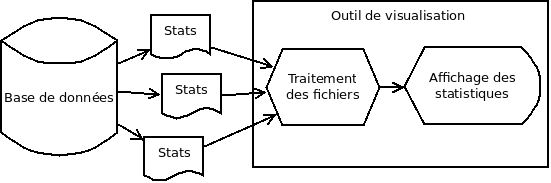
\includegraphics[width=12cm]{images/besoins/visu.png}
	\caption{Processus pour la visualisation des statistiques \label{fig:visu}}
\end{figure}

\paragraph{} On enregistre les statistiques de fonctionnement de la base de données distribuée dans des fichiers. Un outil de visualisation traite ces fichiers et affiche ensuite les statistiques (voir la figure~\ref{fig:visu}).

\newpage
\subsection{Pour en savoir plus...}
Pour nous aider dans le projet, nous avons rechercher des écrits dans plusieurs domaines différents que nous devons aborder. Cette bibliographie initiale est une étude de l'existant. D'autres références sont ensuite disponibles tout au long de ce document, que nous avons trouvé au fil de l'avancement du projet.

\paragraph{Système distribué}

\begin{itemize}
\item Le livre \cite{Ozsu2011} apporte les principes sur les bases de données distribuée. On peut notamment y retrouver des principes sur la réplication ainsi que sur les communications dans le base de données.

\end{itemize}

\paragraph{Algorithmes d'équilibrage de charges}

\begin{itemize}
\item L'article \cite{BalancedAlloc99} met en exergue des algorithmes d'équilibrage, sources d'inspiration pour les clients dans l'élaboration de leurs algorithmes.

\item Le papier \cite{RandomChoices05}, de là même manière que le précédent, s'intéresse de plus près à des algorithmes d'allocation aléatoire. Les deux articles permettent de comprendre l'intérêt des modifications à apporter pour les stratégies de placement et de réplication dans la base de données distribuées.

\item L'article \cite{LoadBalancingPeertoPeer14} traite des algorithmes d'équilibrage des charges dans un réseau pair à pair.

\end{itemize}

\paragraph{Cassandra}

\begin{itemize}
\item Le livre \cite{Hewitt2010} renseigne sur la compréhension du fonctionnement de Cassandra, ainsi que les structures particulières de ce système de base de données.

\item Le lien \cite{ApacheCassandra09} permet d'accéder à l'ensemble de la documentation technique et au dépôt des sources de la base de données Cassandra. On peut y retrouver la documentation côté développeur, pour modifier Cassandra suivant des règles prédéfinies. Les informations sur la compilation du projet et la gestion des tests est aussi présente si l'on se dirige vers le wiki.

\item Le papier \cite{FacebookCassandra09} apporte les explications des créateurs de Cassandra, sur les spécifications de Cassandra par rapport aux autres bases de données du même genre. On y retrouve des informations sur le partitionnement, la réplication et le modèle de données utilisé par Cassandra.

\item Le lien \cite{DSDocCassandra15} possède la documentation la plus complète sur la dernière version de Cassandra, et sur les manières de l'utiliser.
Les nombreux exemples et les approfondissements sont des points d'appuis importants pour le projet. Tous les principes de la base de données sont expliqués de manière globale, sans entrer dans les détails du code source.

\end{itemize}

\paragraph{Visualisation}

\begin{itemize}
\item Le lien \cite{DSOpsCenter14} apporte un logiciel, OpsCenter, capable de montrer graphiquement des statistiques sur une base de données Cassandra opérationnelle. Il peut être utilisé dans le projet, ou apporté des pistes pour la visualisation des données.

\item L'article \cite{Tulip12} s'intéresse à un logiciel de représentation de graphe développé au Labri. Une visualisation sous la forme d'un graphe des données à afficher est tout à fait envisageable. Cet outil nous permettrait de répondre à ce besoin. De plus, ce logiciel est développé au Labri. Nous avons donc des personnes aptes à nous aider à proximité dans le cas de l'utilisation de ce logiciel.
\end{itemize} 



\newpage

\section{Ordonnancement des besoins}

\paragraph{} Nous avons dégagé une liste de besoins fonctionnels et non-fonctionnels. 
Pour mieux les comparer, nous les avons ordonnés en fonction de leur priorité.

\paragraph{} La priorité est un indicateur de l'ordre dans lequel nous devrons implémenter les fonctionnalités afin de satisfaire les besoins du client.

\paragraph{}
\begin{tabular}{| l | M{12cm} |}
    \hline
    Valeur & Signification \tabularnewline
    \hline
    1 & Priorité haute \tabularnewline
    \hline
    2 & Priorité moyenne  \tabularnewline
    \hline
    3 & Priorité faible  \tabularnewline
    \hline
 \end{tabular}


\newpage

\section{Besoins fonctionnels}

\subsection{Communication entre les noeuds}

\paragraph{} Tous les besoins concernent un seul noeud. Tous les noeuds du réseau doivent répondre à ces besoins.

\begin{besoins}
\besoin{Envoyer les informations du noeud à n'importe quel autre noeud}{1}
\besoin{Recevoir les informations provenant d'un autre noeud}{1}
\besoin{Stocker les informations de tous les noeuds du réseau}{1}{
Cela concerne tous les noeuds, y compris soi-même.
}
\end{besoins}

\paragraph{} Les informations d'un noeud doivent permettre d'envoyer un message à ce dernier.



\subsection{Gestion des requêtes}

\paragraph{} Tous les besoins concernent un seul noeud. Tous les noeuds du réseau doivent répondre à ces besoins.


\subsubsection{Requêtes client}

\begin{besoins}
\besoin{Créer une file d'attente des requêtes client}{1}
\besoin{Ajouter une requête à la file d'attente des requêtes client}{1}
\besoin{Défiler une requête de la file d'attente des requêtes client}{1}
\besoin{Traiter une requête client}{1}
\end{besoins}

\begin{besoins}
\besoin{Identifier les noeuds responsables d'un objet}{1}{
Cela nécessite de connaitre plusieurs informations :
\begin{itemize}[noitemsep]
	\item la stratégie de réplication
	\item la token de chaque noeud
	\item le nombre de copie de chaque objet
\end{itemize}
}
\end{besoins}

\begin{besoins}
\besoin{Créer une requête de lecture}{1}{
Les requêtes de lecture doivent être identifiable, ceci afin de pouvoir les supprimer. Il faut donc générer un identifiant pour chaque requête de lecture lors de sa création.
}
\besoin{Envoyer une requête de lecture}{1}
\besoin{Créer une requête d'écriture}{1}
\besoin{Envoyer une requête d'écriture}{1}
\end{besoins}


\subsubsection{Requêtes de lecture}

\begin{besoins}
\besoin{Créer une file d'attente des requêtes de lecture}{1}
\besoin{Recevoir une requête de lecture}{1}
\besoin{Ajouter une requête à la file d'attente des requêtes de lecture}{1}
\besoin{Supprimer une requête de la file d'attente des requêtes de lecture}{1}
\besoin{Défiler une requête de la file d'attente des requêtes de lecture}{1}
\besoin{Traiter une requête de lecture}{1}
\end{besoins}

\begin{besoins}
\besoin{Créer un message de suppression de requête de lecture}{1}
\besoin{Envoyer un message de suppression de requête de lecture}{1}
\besoin{Recevoir un message de suppression de requête de lecture}{1}
\besoin{Traiter un message de suppression de requête de lecture}{1}
\end{besoins}

\begin{besoins}
\besoin{Créer un message de résultat}{1}
\besoin{Envoyer un message de résultat au noeud coordinateur}{1}
\besoin{Recevoir un message de résultat}{1}
\besoin{Transmettre un message de résultat au client}{1}
\end{besoins}


\subsubsection{Requêtes d'écriture}

\begin{besoins}
\besoin{Créer une file d'attente des requêtes d'écriture}{1}
\besoin{Recevoir une requête d'écriture}{1}
\besoin{Ajouter une requête à la file d'attente des requêtes d'écriture}{1}
\besoin{Défiler une requête de la file d'attente des requêtes d'écriture}{1}
\besoin{Traiter une requête d'écriture}{1}
\end{besoins}

\begin{besoins}
\besoin{Créer un message de résultat}{1}
\besoin{Envoyer un message de résultat au noeud coordinateur}{1}
\besoin{Recevoir un message de résultat}{1}
\besoin{Transmettre un message de résultat au client}{1}
\end{besoins}



\subsection{Réaffectation des requêtes de lecture}

\paragraph{} Les besoins sur la réaffectation des requêtes de lecture se recoupent avec ceux de gestion des requêtes de lecture en ce qui concerne les messages envoyés entre les noeuds.

\begin{besoins}
\besoin{Connaître la charge des files d'attentes de requêtes de lecture de chaque noeud du réseau}{1}{Cette information fait partie des informations de chaque noeud, communiqué entre eux comme vu précédemment dans la partie \textit{Communication entre les noeuds}.}
\besoin{Définir un protocole de réaffectation}{1}
\besoin{Modifier le protocole de réaffectation par une configuration}{3}{La configuration est accessible par l'utilisateur, et le protocole de réaffectation doit être la même pour tous les noeuds du réseau}
\besoin{Exécuter le code d'un protocole de réaffectation défini}{1}
\end{besoins}


\subsection{Gestion d'un réseau}

\subsubsection{Popularité d'un objet}

\paragraph{Stockage de la popularité}

\paragraph{} Tous les besoins concernent un seul noeud. Tous les noeuds du réseau doivent répondre à ces besoins.

\begin{besoins}
        \besoin{Créer un vecteur d'entiers comptabilisant le nombre de requêtes}{1}
        \besoin{Augmenter la taille du vecteur}{1} dans le cas où on a l'algorithme qui calcule la popularité de tous les objets
        \besoin{Créer un identifiant permettant de relier la popularité à un objet}{1}
\end{besoins}

\paragraph{Calcul de la popularité}

\paragraph{} Tous les besoins concernent un seul noeud. Tous les noeuds du réseau doivent répondre à ces besoins.

\begin{besoins}
        \besoin{Incrémenter la popularité de l'objet requêté dans le vecteur à chaque requête sur celui-ci}{1}
\end{besoins}

\paragraph{Communication de la popularité}

\paragraph{} Tous les besoins concernent un seul noeud. Tous les noeuds du réseau doivent répondre à ces besoins.

\begin{besoins}
        \besoin{Identifier le noeud responsable d'un objet}{1}
        \besoin{Créer un message de popularité}{1}
        \besoin{Envoyer un message de popularité au noeud responsable de l'objet}{1}
        \besoin{Recevoir un message de popularité}{1}
        \besoin{Traiter un message de popularité (cf paragraphe suivant)}{1}
\end{besoins}

\paragraph{Traitement d'un message de popularité}

\paragraph{} Tous les besoins concernent un seul noeud. Tous les noeuds du réseau doivent répondre à ces besoins.

\begin{besoins}
        \besoin{Stocker la popularité du message dans le vecteur du noeud traitant le message}{1}
        \besoin{Vérifier avoir reçu tous les messages concernant les objets dont le noeud a la gestion}{1}
        \besoin{Décider de créer ou non de nouveau réplicas}{1}
        \besoin{Décider de supprimer ou non des réplicas}{1}
        \besoin{Réinitialiser le vecteur après la création des nouveaux objets les plus populaires}{1}
\end{besoins}

\subsubsection{Réplication d'un objet}

\paragraph{} Tous les besoins concernent un seul noeud. Tous les noeuds du réseau doivent répondre à ces besoins.

\begin{besoins}
        \besoin{Créer une nouvelle stratégie de réplication}{1}
        \besoin{Permettre la définition par l'utilisateur de fonctions de hachage et leur ordre d'utilisation}{1}
        \besoin{Stocker chaque fonction de hachage et son ordre}{1}
        \besoin{Définir un ordre dans les réplicas}{1}
        \besoin{Utiliser la première fonction de hachage pour placer le premier réplica}{1} la seconde pour le second, et ainsi de suite...
        \besoin{Retrouver les réplicas en fonction des fonctions de hachage}{1}
\end{besoins}

\subsection{Application cliente}

\subsubsection{Interactions avec Cassandra}


\begin{besoins}
  	\besoin{Se connecter à Cassandra}{1}
  	\besoin{Se déconnecter de Cassandra}{1}
\end{besoins}
 

\subsubsection{Initialisation des données}

\paragraph{} L'initialisation des données consiste à créer un Keyspace et à enregistrer des données dans celui-ci.

\begin{besoins}
	\besoin{Créer un Keyspace}{1}
	\besoin{Importer des données}{1}
	\besoin{Initialiser les données}{1} Si les données sont modifiées, le client doit pouvoir les initialiser pour revenir aux données d'origine.
\end{besoins}

\subsubsection{Gestion de requêtes}

\paragraph{} Pour tester la validité des algorithmes, l'application devra posséder une fonction de génération de requêtes. 
Si l'utilisateur ne détient pas de suites de requêtes prêtes, il pourra demander à l'application d'en créer pour lui. 
L'application, ne connaissant pas la nature des données, ne pourra qu'effectuer un nombre restreint de requêtes différentes. 
Elle pourra par exemple, compter le nombre de données sauvegardées, chercher si une donnée existe réellement, mais ne pourra pas en modifier une.

\begin{besoins}
  	\besoin{Récupérer le nom des tables}{1} Afin de pouvoir générer des requêtes, nous devons connaître le nom des tables contenues dans un keyspace.
	\besoin{Générer un jeu de données pseudo-aléatoirement}{2} Il s'agit de créer une fonction $f$, qui aura pour ensemble des antécédents des suites de caractères alpha-numériques (par exemple: 5832fg4gh52 ) et pour image un jeu de données.
	\besoin{Importer un jeu de requêtes}{1} L'utilisateur peut importer son propre jeu de requêtes.
\end{besoins}


\subsection{Visualisation des données}

\subsubsection{Sauvegarde des données}

\paragraph{} Afin de suivre l'évolution des charges de chaque noeud lors de l'exécution des algorithmes, on enregistre les données locales de chaque noeud à chaque modification de celles-ci.

\begin{besoins}
  \besoin{Accéder aux données locales de chaque noeud}{1}
  \besoin{Sauvegarder les données locale de chaque noeud}{1} La sauvegarde peut avoir lieu dans un fichier, dans une base de données, dans n'importe quel support nous permettant ensuite de pouvoir récupérer les données.
\end{besoins}

\subsubsection{Affichage des données}

\paragraph{} L'affichage des données locales permet à l'utilisateur de suivre le film de l'exécution des jeux de requête.

\begin{besoins}
 \besoin{Lire les données locales sauvegardées}{1} Selon le format dans lequel elles ont été sauvegardées, un analyseur syntaxique pourrait être utile.
 \besoin{Afficher les données locales}{1} Le format d'affichage importe peu. Il peut s'agir d'un graphique, d'un réseau...
\end{besoins}

\newpage

\section{Besoins non fonctionnels}

\subsection{Cassandra}

\paragraph{} Cassandra est une base de données distribuée.
Nous créons notre environnement distribué à partir de la dernière version stable de Cassandra.

\paragraph{} Le choix de cette solution nous a été fortement recommandé par le client.
En effet, celui-ci dispose de connaissances sur cette application et pourra donc plus facilement intervenir s'il souhaite faire évoluer le projet en implémentant par exemple de nouveaux algorithmes.


\subsection{Maintenabilité du projet}

\paragraph{} L'envergure du projet fait qu'il est possible que d'autres personnes travaillent sur la finalité de ce projet, peu importe son état d'avancement.
Afin de faciliter la compréhension, nous avons défini quelques normes pour que le projet puisse être repris :
\begin{itemize}
	\item documentation dans le code source suivant la norme du langage utilisé;
	\item document externe spécifiant les fichiers modifiés par rapport au code source original;
	\item guide d'installation pour utiliser le projet et pour modifier le projet.
\end{itemize}

\subsection{Visualisation des données}


\paragraph{} L'état du réseau doit être visible en temps réel.

\paragraph{} La vue peut donc être actualisée toutes les $0.5$ secondes. 
Un délai plus faible risquerait de ralentir le système, étant donné que l'obtention des données nécessaires à la visualisation se fait sur la même base de données que celle qui est testée.


\newpage
\section{Gestion de projet}

\subsection{Répartition des tâches}

\subsubsection{Diagramme de Gantt}

\rotatebox{270}{
\begin{ganttchart}[
hgrid,
vgrid={*6{blue,dashed}, *1{red}},
inline = true,
x unit=4mm,
time slot format=isodate,
milestone inline label node/.append style={left=3mm},
y unit chart = 0.45cm,
bar top shift= 0.1,
bar height = 0.8
]{2015-02-16}{2015-04-08}
\gantttitlecalendar{month=name, day} \\

\ganttgroup{Gestion des requêtes (A)}{2015-02-16}{2015-03-06} \\
\ganttbar[name=a1]{A1}{2015-02-16}{2015-02-18} \\ %Envoi des requêtes de lecture
\ganttbar[name=a2]{A2}{2015-02-19}{2015-02-25} \\ %Suppression des requêtes de lecture
\ganttbar[name=a3]{A3}{2015-02-26}{2015-03-02} \\ %Gestion des messages de suppression d'une requête
\ganttbar{AT}{2015-03-03}{2015-03-06} \\ %Tests

\ganttgroup{Réaffectation des requêtes de lecture (B)}{2015-03-07}{2015-03-29} \\
\ganttbar{B1}{2015-03-07}{2015-03-14} \\ %Système d'assignation d'une requête
\ganttbar{B2}{2015-03-07}{2015-03-14} \\ %Communication charge file d'attente
\ganttbar{B3}{2015-03-15}{2015-03-24} \\ %Algorithme SLVO
\ganttbar{B4}{2015-03-15}{2015-03-24} \\ %Algorithme AvergeDegree
\ganttbar{BT}{2015-03-25}{2015-03-29} \\ %Tests

\ganttgroup{Gestion de la réplication (C)}{2015-02-16}{2015-03-07} \\
\ganttbar{C1}{2015-02-16}{2015-02-19} \\ %Créer une nouvelle stratégie de réplication
\ganttbar{C2}{2015-02-20}{2015-03-02} \\ %Chaque fonction de hachage pour les réplicas
\ganttbar{C3}{2015-02-20}{2015-03-02} \\ %Retrouver chaque réplica grâce aux fonctions de hachage
\ganttbar{CT}{2015-03-03}{2015-03-07} \\ %Tests

\ganttgroup{Gestion de la popularité (D)}{2015-03-08}{2015-03-29} \\
\ganttbar{D1}{2015-03-08}{2015-03-15} \\ %Calcul de la popularité pour un objet
\ganttbar{D2}{2015-03-16}{2015-03-20} \\ %Implémentation de SpaceSaving
\ganttbar{D3}{2015-03-21}{2015-03-27} \\ %Simulateur
\ganttbar{DT}{2015-03-28}{2015-03-29} \\ %Tests

\ganttgroup{Application cliente (E)}{2015-02-16}{2015-03-10} \\
\ganttbar{E1}{2015-02-16}{2015-03-05} \\ %Gestion Cassandra
\ganttbar{E2}{2015-02-27}{2015-03-05} \\ %Générateur de requêtes et d
\ganttbar{ET}{2015-03-06}{2015-03-10} \\ %Tests

\ganttgroup{Visualisation des données (F)}{2015-03-10}{2015-03-28} \\
\ganttbar{F1}{2015-03-10}{2015-03-15} \\ %Prise en main Graphite
\ganttbar{F2}{2015-03-16}{2015-03-21} \\ %Ajout metrics
\ganttbar{F3}{2015-03-22}{2015-03-28} \\ %Paramétrage

\ganttbar{T}{2015-04-01}{2015-04-04} \\

\ganttmilestone{Livrable final}{2015-04-08} 

\end{ganttchart}
}


\newpage

\subsubsection{Affectation des tâches}

\paragraph{}
\begin{tabular}{| l | M{5cm} | M{3cm} | M{5.5cm} |}
    \hline
    Fct & Description & Développeur(s) & Commentaire \tabularnewline
    \hline
    A1 & Envoi des requêtes de lecture & Kévin & Court-circuitage du système de digest de Cassandra  \tabularnewline
    \hline
    A2 & Suppression des requêtes de lecture & Kévin &  \tabularnewline
    \hline
    A3 & Gestion des messages de suppression d'une requête & Kévin & Envoi/réception/traitement \tabularnewline
    \hline
    AT & Tests groupe A & Kévin &  Vérification, tests, mémoire \tabularnewline
    \hline 
    \hline
    B1 & Système d'assignation d'une requête & Kévin & Ne pas envoyer les messages de suppression plusieurs fois  \tabularnewline
    \hline
    B2 & Communication charge file d'attente & Kévin & Voir Gossip \tabularnewline
    \hline
    B3 & Algorithme SLVO & Kévin & Base modulaire  \tabularnewline
    \hline
    B4 & Algorithme AvergeDegree & Kévin & Base modulaire  \tabularnewline
    \hline
    BT & Tests groupe B & Kévin &  Vérification, tests, mémoire \tabularnewline
    \hline
    \hline
    C1 & Stratégie de réplication & Corentin  & Nouvelle stratégie \tabularnewline
    \hline
    C2 & 1 fonction de hachage par niveau de réplica & Corentin  &  \tabularnewline
    \hline
    C3 & Retrouver les réplicas grâce aux fonction de hachage & Corentin  &  \tabularnewline
    \hline
    CT & Tests groupe C & Corentin & Vérification, tests, mémoire \tabularnewline
    \hline
    \hline
    D1 & Calcul de la popularité d'un objet & Corentin & Temps de recherche et exploration des mécanismes  \tabularnewline
    \hline
    D2 & SpaceSaving Algorithm & Corentin & Temps de recherche et exploration des mécanismes \tabularnewline
    \hline
    D3 & Simulateur & Corentin & Développement Simulateur \tabularnewline
    \hline
    DT & Tests groupe D & Corentin & Sur Simulateur \tabularnewline
    \hline
    \hline
    E1 & Gestion de Cassandra & Guillaume &  Développement de l'application et utilisation pilote \tabularnewline
    \hline
    E2 & Générateur de requêtes &  Guillaume & \tabularnewline
    \hline
    ET & Tests groupe E &  Guillaume &  Vérification, tests et mémoire \tabularnewline
    \hline
    \hline
    F1 & Prise en main de Graphite & Guillaume & Installation, tests \tabularnewline
    \hline
    F2 & Ajout de metrics & Kévin et Guillaume &  Mesure de la charge d'un noeud \tabularnewline
    \hline
    F3 & Paramétrage &  Guillaume &  Paramétrage de la web app \tabularnewline
    \hline
    \hline
    T & Tests finaux & * &  Vérification, tests, mémoire \tabularnewline
    \hline
\end{tabular}
 
\newpage
 
\subsection{Outils utilisés}

\subsubsection{Flowdock}

\paragraph{}Flowdock est un outil de travail d'équipe. Il permet un dialogue entre les membres grâce au Chat intégré, un partage facile de fichiers et il affiche les dernières modifications réalisées sur des outils annexes (comme les derniers commits sur le dépôt GitHub ou les derniers post-it de Trello). Il est également disponible sur mobile avec une application dédiée.

\paragraph{}Bien pratique, Flowdock a permis de concentrer en un unique endroit les avancées du projet et permet un énorme gain de temps, sur la recherche et la gestion des informations.

\subsubsection{Trello}

\paragraph{}Trello est une sorte de grand mur à post-it. L'organisation des tâches, des rendez-vous, le partage des documents, tout est facilité. Classés en différentes catégories, les fiches de Trello permettent en un clin d'oeil de voir le travail effectué, en cours ou restant à faire. Il possède une gestion de label qui permet de chercher rapidement ce que l'on souhaite.

\paragraph{}Nous avons utilisé Trello pour la répartition du travail et le découpage des tâches. Disponible également sur mobile, nous avons délégué à la plateforme la gestion des plannings du projet.

\subsubsection{Git - Svn}

\paragraph{}Git et Svn sont deux gestionnaires de version largement connus. Nous avons utilisé Git pour sa facilité de mise en oeuvre (avec GitHub) et sa possibilité de travailler en local. Les liens ont été faits à chaque fois entre le dépôt Git et Svn (à chaque rendez avec le chargé de TD par exemple).

\newpage

\section{Architecture}
\label{sec:Architecture}



\subsection{Application cliente}

\paragraph{} Pour communiquer avec la base de données, nous utilisons un \textit{pilote}, programme informatique permettant à un programme d'intéragir avec un autre programme.

\subsubsection{Présentation du pilote}
\paragraph{} Le pilote que nous utilisons est Java Driver 2.0 for Apache Cassandra développé par l'entreprise Datastax, distributeur de Cassandra. Le pilote est sous licence Apache.

\paragraph{} L'entreprise Datastax étant très spécialisé dans le développement de logiciels centrés sur Cassandra, son pilote est le plus complet. Il propose
toutes les fonctionnalités dont nous avons besoin.

\begin{figure}[h]
	\centering
		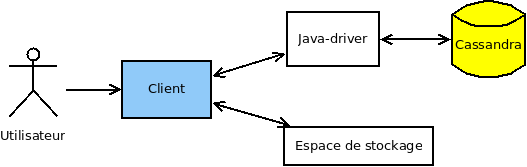
\includegraphics[width=12cm]{images/client/acteurs.png}
	\caption{Interactions du client \label{fig:client_acteurs}}
\end{figure}

\paragraph{} Sur la figure~\ref{fig:client_acteurs}, l'application cliente est représentée par le rectangle bleu nommé client.
Le client exécute les actions souhaitées par l'utilisateur. Les communications entre l'application cliente et la base de données Cassandra passent par le java-driver.
Le client peut lire et écrire des fichiers dans l'espace de stockage.

\subsubsection{Architecture de l'application cliente}

\begin{figure}[h]
	\centering
		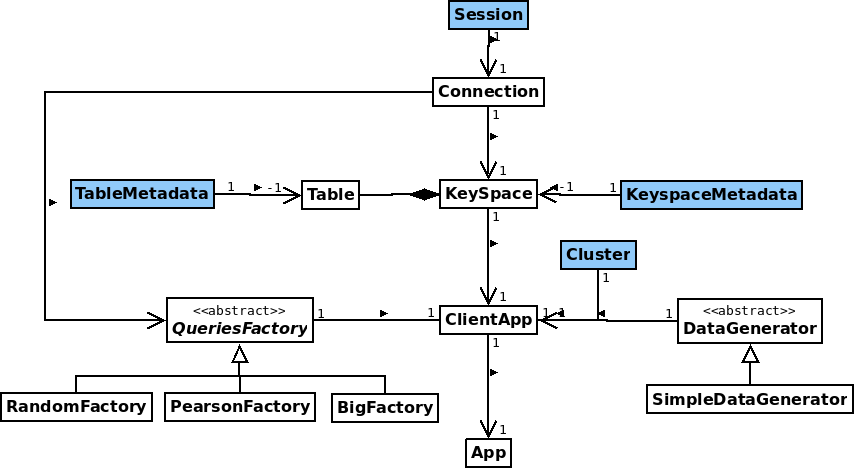
\includegraphics[width=12cm]{images/client/diagumlclient.png}
	\caption{Diagramme de classes simplifié de l'application cliente \label{fig:client_uml}}
\end{figure}

\paragraph{} 

\paragraph{} Les classes du java-driver sont bleues dans la figure~\ref{fig:client_uml}.
\begin{itemize}
 \item La classe \class{Cluster} crée des objets permettant la connexion à la base de données Cassandra.
 \item La classe \class{Session} crée des objets permettant d'envoyer des requêtes au format Cassandra Query Language (CQL) à Cassandra. 
 \item La classe \class{KeyspaceMetadata} crée des objets permettant de récupérer les informations principales concernant un keyspace.
 Par exemple, le nom du keyspace, les tables stockées ou bien la classe pour la stratégie de réplication utilisée.
 \item La classe \class{TableMetadata} crée des objets permettant de récupérer les informations principales concernant une table.
 Par exemple, le nom de la table ou les colonnes composant la table.
\end{itemize}

\paragraph{} A partir de ces quatres classes, nous avons développé l'architecture de l'application cliente.
\begin{itemize}
 \item La classe \class{App} contient le \class{main}.
 \item L'objet \class{ClientApp} est le coeur de l'application. C'est l'objet qui communique et exécute les actions que souhaite effectuer l'utilisateur.
 \item La classe \class{Table} crée un objet contenant les informations propre à une table donnée.
 \item La classe \class{KeySpace} crée un objet contenant les informations propre à un keyspace donné.
 \item L'objet \class{Connection} permet d'exécuter des requêtes sur la base de données.
 \item Les objets héritant de \class{QueriesFactory} sont des générateurs de requêtes, ils envoient des suites de requêtes à Cassandra.
 \item Les objets héritant de \class{DataGenerator} sont des générateurs de données, ils permettent de génerer des données pour effectuer les simulations.
\end{itemize}


\subsection{Visualisation des métriques}

\paragraph{} Pour visualiser les métriques, nous utilisons l'application nommée \path{Graphite} écrite en Python.

\paragraph{} Graphite est l'union de trois logiciels:
\begin{itemize}
 \item \textbf{carbon}, un logiciel permettant de traiter des données temporelles, comme l'évolution de la charge d'un noeud en fonction du temps.
 \item \textbf{whisper}, une base de données stockant toutes ces données
 \item \textbf{graphite webapp}, une application web permettant la visualisation de ces données.
\end{itemize}

\begin{figure}[h]
	\centering
		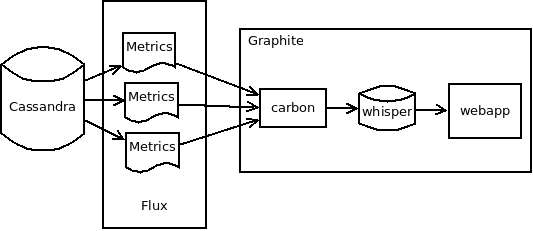
\includegraphics[width=12cm]{images/client/graphite.png}
	\caption{Graphite, union de trois logiciels \label{fig:client_visu}}
\end{figure}


\paragraph{} Les métriques sont directement envoyées à Graphite en créant une connexion entre le metrics de Cassandra et Graphite, voir figure~\ref{fig:client_visu}
Pour cela, on utilise l'objet \class{GraphiteReporter} dans le module \class{metrics-graphite}.

\paragraph{} Ces données sont ensuite traitées par Carbon puis sauvegardées dans la base de données Whisper.
Enfin, la web-app de Graphite affiche ces informations sous forme de graphes (courbes, histogrammes...) dans un navigateur web.

\paragraph{} L'utilisation de cette application permet de visualiser un grand nombre de métrics déjà disponible dans la version originale de Cassandra.
On peut citer par exemple, le volume total de données stockées sur un cluster, le temps de lecture des données, la taille totale du cache...
En ajoutant un metric pour mesurer la charge d'un noeud, on peut visualiser celle-ci au cours du temps grâce au divers formats de graphiques proposés par Graphite.


\newpage 
\section{Réalisation du projet}

\subsection{Modification de Cassandra}

\paragraph{}Une partie importante du projet consiste à adapter le comportement de la base de données Cassandra afin de répondre aux besoins. Nous avons décidé de travailler sur la version \textbf{2.1.2}, dernière version stable au début du projet. La modification du code source de Cassandra demande, outre la création de code, des compétences de lecture et de compréhension de code. En effet, il n'existe pas de documentation officielle concernant le code source de Cassandra. On peut tout de même retrouver des explications sur l'architecture interne dans le wiki officiel hébergé par la fondation Apache \cite{CassArchi13} ainsi que d'autres détails sur la documentation réalisée par Datastax \cite{DatastaxDoc15}.

\paragraph{}Dans la mesure du possible, nous avons respecté les conventions de codage de Cassandra \cite{CassCodeStyle14}, elles mêmes découlant des conventions de codage Java créées par Sun.

\paragraph{}La majeur partie du projet, pour la modification de Cassandra, a consisté en sa compréhension, car pour modifier un comportement, il faut d'abord connaître celui qui existe. C'est pourquoi l'architecture du projet s'est construite en même temps que son implémentation (l'architecture représentant bien 4 ou 5 fois plus de temps que l'implémentation). Pour trouver les points d'intérêt dans le code (cheminement d'une requête de lecture par exemple), l'utilisation des \textit{logs} est primordiale. Couplé à un environnement de travail (IDE) permettant l'usage du \textit{"Go To Definition"} (permet de retrouver instantanément, à partir d'un endroit où une fonction est utilisée, l'endroit où elle est définie), nous avons alors pu retracer efficacement différentes parties de Cassandra sur lesquels nous avons travaillé. Les diagrammes de classes et de séquences de l'architecture ont été créé à partir de cette méthode (mais ils sont fortement simplifiés pour faciliter leur compréhension).

\subsubsection{Outils utilisés}

\subsubsection*{CCM}

\paragraph{}CCM (Cassandra Cluster Management) est un script/bibliothèque écrit en Python permettant de gérer facilement un cluster de Cassandra sur une machine locale. Il a été développé par Sylvain Lebresne, développeur chez Datastax (entreprise spécialisée dans Cassandra), et est dynamique dans son évolution avec des mises à jour constantes depuis plusieurs années. C'est pourquoi nous avons choisi cet outil pour nous aider dans notre développement.

\paragraph{}Il faut savoir que chaque instance de Cassandra correspond à un noeud, et qu'une instance est faite pour fonctionner sur chaque machine du réseau (un noeud équivaut à une machine). Mais en phase de développement et de tests, on souhaite pouvoir lancer un cluster entier sur une seule machine, ce qui n'est pas aisé à faire. C'est ici que CCM intervient en automatisant la création/gestion/suppression d'un cluster Cassandra en local.

\paragraph{}Son installation est peu triviale et son utilisation n'est pas dénuée de bugs, mais dans l'ensemble, CCM nous a apporté un gain de temps très important dans la réalisation de ce projet.

\paragraph{}Ainsi, la création, le lancement et la destruction d'un cluster se déroule de la manière suivante. Tout d'abord, on crée un cluster à partir des fichiers sources de Cassandra.
\shellcmd{py ccm create nom\_cluster --install-dir=<chemin\_de\_cassandra>}

Ensuite, on ajoute des noeuds à ce cluster. Ici on décide d'en créer 3. C'est à ce moment que toute la configuration de noeuds se fait de manière automatique, une étape longue et critique lorsqu'elle est réalisée à la main.
\shellcmd{py ccm populate -n 3}

On peut alors lancer le cluster, qui va se charger des créer les instances de Cassandra pour chaque noeud du réseau.
\shellcmd{py ccm start}

Lorsqu'on a fini de réaliser nos tests, on peut ensuite arrêter les instances de Cassandra tournant en fond de tâche.
\shellcmd{py ccm stop}

Il est à noté que si l'on veut relancer le même cluster, il suffit de refaire la commande de lancement sans repasser par les étapes précédentes. Le cluster ainsi que les données qu'il possède ne sont pas supprimé. Mais si on veut le faire, alors il suffit d'une commande.
\shellcmd{py ccm remove}

\subsubsection*{Class Visualizer}

\paragraph{}Class Visualizer est un outil de visualisation de code Java sous la forme d'un diagramme de classes UML. Il est très utile pour comprendre les relations entre les classes dans un projet. Cependant, la structure particulière de Cassandra (nombreux singletons statiques) ne permet pas d'utiliser toute la puissance de cet outil car il n'arrive pas à retrouver les liens de dépendances entre les classes. Nous nous sommes donc peu servi de cet outil.

\subsubsection{Affectation des requêtes de lecture}

\subsubsection*{Solution implémentée}

\paragraph{}Lors d'une requête de lecture, le comportement par défaut de Cassandra est d'envoyer la requête de lecture au noeud possédant l'objet \textit{"le plus proche"} (défini suivant la configuration) qui doit renvoyer la donnée, et d'envoyer la requête de lecture à plusieurs autres noeuds possédant une copie de l'objet qui doivent renvoyer un \textit{digest}, correspondant à un hash MD5 de la donnée demandée. Le nombre de noeuds auquel on envoie une requête de type \textit{digest} est paramétrable grâce au niveau de consistance. Ainsi, une consistance de 1 ne demandera pas de \textit{digest} et sera donc plus rapide, mais la donnée ne sera pas forcément la plus récente. Car l'intérêt du \textit{digest} est de pouvoir comparer la valeur de l'objet demandé sur plusieurs noeuds pour essayer au maximum de donner la valeur la plus récente. Mais envoyer la donnée est plus gourmand sur le réseau qu'envoyer un valeur de hash, c'est pourquoi cette technique est utilisée. On attend une réponse de chaque noeud concerné pour pouvoir répondre à la requête.

\paragraph{}Dans notre cas, nous voulons comme comportement envoyer une requête de lecture à \textbf{tous} les noeuds possédant une copie, quelque soit le niveau de consistance, et en leur demandant de renvoyer la \textbf{donnée complète}, donc sans \textit{digest}. On répond ensuite à la requête dès qu'\textbf{un} noeud à répondu.

\paragraph{}Pour implémenter ce comportement, nous avons modifier la classe \class{AbstractReadExecutor} pour qu'elle nous renvoie une instance qui n'utilise pas de \textit{digest}, instance de la classe \class{NoDigestReadExecutor} que nous avons créé (voir figure~\ref{fig:read_diagram_modified}). De plus, elle envoie une requête à tous les noeuds, peu importe le niveau de consistance. Pour créer des \class{NoDigestReadExecutor}, il a fallu empêcher la création des autres classes (ce sont toutes des classes privées statiques contenues dans \class{AbstractReadExecutor}), créées à partir de la méthode \texttt{getReadExecutor}. Seule notre nouvelle classe peut maintenant être instanciée.

\paragraph{}Un autre point important concerne la suppression d'une requête de lecture. Par défaut, c'est un comportement qui n'existe pas dans Cassandra, et qui n'a certainement pas été imaginé possible au vu de l'implémentation. La première chose que nous avons réalisé est d'envoyer des requêtes pouvant être supprimées dans les files d'attentes, avec des méthodes différentes de celles pouvant être supprimées. Si l'on reprend la figure~\ref{fig:read_diagram_modified}, on peut remarquer un changement dans les messages envoyés au stage de lecture. On a réutilisé les fonctions précédentes mais en ajoutant "Removable" à la fin de leur nom pour les différentier.

\paragraph{}Pour comprendre comment supprimer une requête de la file d'attente, il faut comprendre ce qu'il y a dans une file d'attente. Si l'on regarde l'architecture d'un stage (voir figure~\ref{fig:stages_diagram}), on s'aperçoit qu'une requête dans la file d'attente sera représenté par une instance de \class{FutureTask}. Or, ce que l'on souhaite supprimer correspond à une instance de \class{ReadCommand} (la classe gérant la requête de lecture). Il a donc fallu trouver un système pour comparer ces deux classes. La première chose a été d'ajouter une classe \class{RemovableFutureTask} pour gérer les requêtes pouvant être supprimées de la file d'attente (voir figure~\ref{fig:stages_diagram_modified}). Cette classe possède la particularité de laisser la vérification de l'égalité de la classe à son attribut \textit{runnable} (qui correspond au \textit{callable} de \class{FutureTask} avant sa transformation). Ainsi, si l'on cherche à supprimer une requête de la file d'attente en envoyant une instance de \class{ReadCommand}, on compare cette instance au objet de la file d'attente, qui eux-même passeront par leur attribut \textit{runnable}, et ainsi de suite jusqu'à retrouver l'objet de \class{ReadCommand} original (voir figure~\ref{fig:remove_request_diagram}).

\begin{figure}[!h]
	\centering
        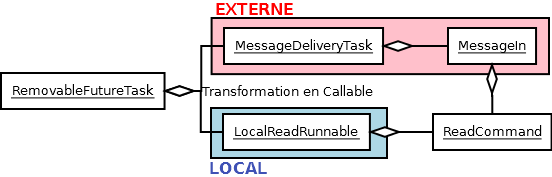
\includegraphics[width=13cm]{images/implementation/remove_request_diagram.png}
    \caption{Classes redéfinissant la méthode \textit{equals} pour pouvoir comparer et supprimer des requêtes de lectures \label{fig:remove_request_diagram}}
\end{figure}

\paragraph{}Les instances de \class{ReadCommand} sont identifiées et comparées grâce à leur attribut "timestamp" et "key".

\paragraph{}Maintenant qu'il est possible de supprimer une requête de lecture d'une file d'attente, il faut s'intéresser à l'envoi/réception d'un message de suppression, ainsi qu'à son traitement. Nous avons donc créer un nouveau stage pour gérer ces messages : le stage \textbf{READ\_REMOVE}. Il est mono-threadé, contrairement au stage de lecture qui est multi-threadé (32 threads par défaut).

\paragraph{}Les messages qu'il traite sont les verbes \textbf{READ\_REMOVE} dont le traitement se fait dans la classe \class{ReadRemoveVerbHandler}. La création d'un message se fait à partir de \class{ReadCommand} avec la méthode \texttt{createRemoveMessage}, qu'il suffit alors d'envoyer aux autres noeuds par le biais du \class{MessagingService}. Cette tâche est donnée à la classe \class{AsbtractReadExecutor} et sa méthode \texttt{makeRemoveRequests}.

\subsubsection*{Problèmes et limites rencontrés}

\paragraph{}La suppression d'une requête de la file d'attente de lecture a été une partie compliquée, car les relations entre les objets dans une file d'attente et les objets que l'on cherche à comparer ne sont pas évidentes à retrouver.

\paragraph{}Il a aussi fallu faire attention à la concurrence étant donné que nous travaillons dans un environnement multi-threadé. C'est pourquoi nous utilisons la méthode native de suppression d'une file (représentée en interne par une \class{ConcurrentLinkedQueue}) pour assurer une meilleure sécurité. C'est ce qui nous a conduit à choisir comme solution de redéfinir les méthodes \textit{equals}.

\paragraph{}Le dernier point qu'il a fallu prendre en compte est qu'il y a deux manières de faire une requête : local et externe. Il faut donc s'assurer que les deux manières de faire sont traitées. Le fait d'avoir ces deux manières est un gain de temps en production, mais complexifie cependant la compréhension et la lisibilité du code.

\subsubsection*{Travail restant à réaliser}

\paragraph{}Cette partie du projet a été réalisé entièrement. On peut malgré tout s'interroger sur une méthode plus efficace (en terme de lisibilité) pour traiter la suppression d'une requête. Mais cela nécessiterait de chambouler un peu plus le code original, et un travail beaucoup plus important pour s'assurer que le comportement de Cassandra n'est pas altéré.

\paragraph{}Des tests sur le nombre de threads accordés au stage de suppression de requête seraient aussi intéressant. L'augmentation de threads provoquerait une diminution du traitement des autres stages, mais augmenterait la vitesse de suppression des requêtes, permettant alors d'en traiter moins en plusieurs exemplaires.

\paragraph{}Les attributs permettant d'identifier les requêtes sont aussi à revoir. Actuellement, le \textit{timestamp} n'est pas la valeur la plus sûre car il est toujours possible que deux requêtes identiques soient lancées au même moment par deux clients différents. Une possibilité seraient de générer un identifiant aléatoirement pour chaque instance de \class{ReadCommand}. Le risque de collision avec cet identifiant couplé au timestamp serait alors quasiment nul. Cela demanderait alors de modifier les \textit{serializer} pour être capable de transmettre cette donnée dans un message.

\subsubsection{Réaffectation des requêtes de lecture}

\subsubsection*{Solution implémentée}

\paragraph{}Charge des files d'attente des requêtes de lecture (avec gestion de la décrémentation lorsqu'une requête est traitée) grâce à un compteur. Communication de la charge à tous les autres noeuds du réseau (Gossiper, ApplicationState, LoadReadBroadcaster, versionedValue).

\paragraph{}Dans le projet, nous devons implémenter un système permettant, pour chaque noeud, de s'affecter toutes les requêtes de lecture de sa file d'attente. Cette décision se prend suivant un protocole de réaffectation, qui doit être modifiable facilement.

\paragraph{}Pour prendre cette décision, il est nécessaire d'avoir comme information la \textit{charge} de chaque noeud du réseau pour la file d'attente des requêtes de lecture. Cela implique d'avoir cette donnée localement, de pouvoir la modifier, et de pouvoir la transmettre aux autres noeuds.

\paragraph{}Cette donnée se situe dans la classe \class{SEPExecutor} sous l'attribut \texttt{effectiveLoad}. Chaque fin de traitement de requête de lecture entraîne la décrémentation du compteur (si la valeur actuelle du compteur est supérieure à 0). Le point important est d'utiliser un type permettant de gérer la concurrence (environnement multi-threadé). C'est pourquoi nous utilisons le type \class{AtomicLong} spécialement prévu pour cet effet.

\paragraph{}Maintenant que nous possédons un compteur du nombre de tâches affectées, il est facile de retrouver le nombre de tâches non affectées (un compteur de tâches en attentes existe déjà). Il faut alors communiquer cette donnée. Pour ça, nous avons ajouté cette information à celle déjà présente dans les communications Gossip (voir la section~\ref{sec:Architecture}) entre les noeuds.

\paragraph{}Cet ajout se déroule en plusieurs étapes. Tout d'abord, nous avons ajouté la donnée \textbf{READ\_LOAD} dans \class{ApplicationState}, permettant de dire ce qu'on transmet entre les noeuds. Le \class{Gossiper} transmettra l'information contenu dans \textbf{READ\_LOAD}.

\paragraph{}Ensuite, nous avons créé une classe qui gère la relation entre le \class{Gossiper} et le reste de l'application : \class{LoadReadBroadcaster}. Son rôle est, à intervalle régulier, de mettre à jour l'information de \textbf{READ\_LOAD} à partir de l'information du \class{SEPExecutor} du stage de lecture. C'est aussi à partir de lui que l'on peut récupérer les informations de la charge de tous les autres noeuds du réseau à partir de sa méthode \texttt{getLoadInfo}.

\subsubsection*{Problèmes et limites rencontrés}

\paragraph{}La solution actuelle se base sur un compteur pour déterminer les requêtes qui ont été affectées dans la file d'attente. Cependant, l'aspect multi-threadé peut, plus tard, poser des problèmes. En effet, il se peut que le compteur ne soit pas parfaitement en adéquation avec les requêtes que nous nous sommes assignées, et pour lesquels nous avons envoyé des requêtes de suppression aux autres noeuds. On enverrai alors des requêtes de suppression lors du traitement de la requête de lecture alors qu'on avait déjà envoyé ces requêtes auparavant lors de l'affectation.

\paragraph{}Le risque est alors d'envoyer des messages inutiles dans le réseau. Le contraire n'est pas possible si on modifie la charge avant de parcourir la file d'attente pour envoyer les messages de suppressions (cela aurait été plus problématique car il n'y aurait pas eu de réponse à la requête du client du coup).

\paragraph{}Une autre solution, plus couteuse en terme de temps de développement, serait de créer une nouvelle file d'attente pour les requêtes affectées, et de basculer les requêtes dans cette file lorsque l'on veut l'assigner à ce noeud.

\subsubsection*{Travail restant à réaliser}

\paragraph{}Nous n'avons pas réalisé tous les objectifs dans cette partie par manque de temps. Il reste de nombreux points à aborder pour achever ce travail, mais ils ont été tout de même réfléchi.

\paragraph{}Il faut encore exécuter le protocole de réaffectation, qui doit être  lancé dès que l'on traite une requête de lecture ou de suppression. Ce protocole doit vérifier les conditions d'exécution qui lui sont propres (SLVO ou AverageDegree ne possèdent pas les mêmes conditions), et si elles passent, doit modifier la charge et parcourir la file d'attente pour envoyer un message de suppression à tous les autres noeuds possédant ces mêmes requêtes.

\paragraph{}Une requête affectée ne doit pas entrainer de message de suppression lors de son traitement car ils ont été réalisés plus tôt par le système de réaffectation. L'idée serait de marquer les requêtes (un booléen par exemple) pour indiquer si elles sont affectées ou non.

\paragraph{}Le dernier point concerne la configuration du protocole de réaffectation. Il est nécessaire de pouvoir le modifier facilement afin de comparer les résultats sur les performances des différents protocoles. La solution envisagée est d'utiliser le même système qui est actuellement en place pour configurer la réplication : un système de réflexion paramétrable pour chaque Keyspace, où il suffit de rentrer le nom de la classe du protocole de réaffectation lors de la création d'un Keyspace.

\subsubsection{Réplication des objets}

\subsubsection*{Solution implémentée}

\paragraph{}Après discussion avec la communauté de développeurs de Cassandra, une solution de placement a été implémentée. En effet, pour rappeler le besoin sur le placement des copies, il a été souhaité que le placement de l'objet initial se fasse avec une fonction de hachage $ H_0 (c) $ avec $c$ la clé primaire de l'objet. Le placement des réplicas devait s'effectuer à l'aide de la fonction $ H_1 (c) $ pour la première copie, $H_2 (c) $ pour la deuxième copie et ainsi de suite.

\paragraph{}La méthode implémentée consiste à utiliser la fonction $ H_0 (c) $ pour le placement initial. Le premier réplica est placé grâce à $ H_1 (H_0 (c)) $, le second grâce à $ H_2 (H_0 (c)) $ et ainsi de suite.

\paragraph{}La création de cette implémentation a nécessité la création d'une nouvelle stratégie de réplication nommée \class{MultiHashStrategy}. Elle peut être utilisée comme n'importe quelle stratégie de réplication, c'est à dire qu'il suffit d'indiquer son nom lors de la création d'une keyspace. Il est a noté que cette stratégie ne fonctionne correctement qu'avec la méthode de répartition en \textbf{Murmur3}, car cette stratégie utilise des fonctions de hachages Murmur3. Si on utilise une autre méthode de répartition, la distribution des copies ne sera plus uniforme.

\subsubsection*{Problèmes et limites rencontrés}

\paragraph{}Outre la difficulté à comprendre les mécanismes de Cassandra, plusieurs problèmes se sont posés à nous. En effet, la communication de la clé primaire d'un objet n'est pas possible immédiatement dans le développement de nouvelles stratégies. Il faudrait modifier le comportement de plusieurs autres classes, ce qui nous était difficile durant le temps imparti. Le comportement a légèrement été modifié comme décrit ci-dessus.

\paragraph{}Un autre aspect (mineur dans notre projet) est que cette fonctionnalité entraîne une perte de la capacité de Cassandra à s'adapter à son réseau. En effet, Cassandra est conçu pour se reconfigurer facilement lors d'ajout ou de suppresion de noeuds dans son réseau. Cependant, dans notre projet, nous nous intéressons à un réseau de taille fixe qui n'évoluera pas dans le temps.

\paragraph{}Et enfin, il est important de mesurer les différences entre les deux solutions. Effectivement, si elles se ressemblent sur leur principe, un point important est à noter : une différence forte au niveau des collisions. Une \textit{collision} est lorsqu'une fonction de hachage retourne la même valeur pour deux entrées différentes. \newline
Prenons par exemple, le cas de deux objets ayant pour clé primaire $c1$ et $c2$ et avec $ H_0 (c1) = k $ et $ H_0 (c2) = k $ (nous avons donc une collision).
\begin{itemize}
    \item \underline{Solution initiale :} \newline
        Placement initial : $ H_0 (c1) = k $ et $ H_0 (c2) = k $ \newline
        Premier réplica : $ H_1 (c1) = k1 $ et $ H_1 (c2) = k2 $ avec $ k1 \neq k2 $ sauf si $ H_1 (c1) = H_1 (c2) $ \newline 
        Avec une collision sur le placement de la donnée initiale, la probabilité d'avoir les premiers réplicas sur le même noeud dépend du domaine de collision de la fonction $ H_1 $.


    \item \underline{Solution implémentée :} \newline
        Placement initial : $ H_0 (c1) = k $ et $ H_0 (c2) = k $ \newline
        Premier réplica : $ H_1 (H_0 (c1)) = H_1(k) = k3 $ et $ H_1 (H_0 (c2)) = H_1(k) = k3 $ \newline
        Second réplica : $ H_2 (H_0 (c1)) = H_2 (k) = k4 $ et $ H_2 (H_0 (c2)) = H_2 (k) = k4 $ \newline
        Avec une collision sur le placement de la donnée initiale, toutes les copies seront placées sur le même noeud deux à deux. \newline
        Autrement dit, toutes les données qui entrent en collision pour la première fonction de hachage, auront leur premier réplica sur le même noeud $Y$ et ainsi de suite.

\end{itemize}

On a une donc une répartition des données moins efficace car si on avait une collision, on souhaitait que les réplicas ne soit pas sur les mêmes noeuds pour ces données. Toutefois, le risque de collision reste assez faible car la fonction de hachage Murmur3 donne des résultats codés sur 64 bits (le type \textit{Long} en Java), soit $2^{64}-1$ solutions possibles.

\subsubsection*{Travail restant à réaliser}

\paragraph{}Bien que l'ensemble de la partie ait été réalisée, il n'est pas aisé de changer de fonction de hachage. En effet, si l'utilisateur souhaite utiliser de nouvelles fonctions de hachage, il doit recréer une nouvelle stratégie de réplication et recompiler l'ensemble. On pourrait alors imaginer une stratégie de réplication qui charge des fonctions de hachage grâce à des paramètres fournis à l'exécution.

\subsubsection{Popularité des objets}

\subsubsection*{Solution implémentée}

\paragraph{}Aucune solution technique n'a été implémentée. Cependant, les réflexions sur le développement ont avancé. Le point est fait dans la partie \textit{Travail restant à réaliser}.

\subsubsection*{Problèmes et limites rencontrés}

\paragraph{}Créer un mécanisme de popularité est un gros ajout dans Cassandra qui nécessite la modification (et donc la compréhension) d'un ensemble de mécanismes. En effet, nous intervenons au niveau des requêtes pour compter leur nombre et savoir quel objet elles vont utiliser. S'ajoutent ensuite la communication réseau pour transmettre le nombre total de requêtes et la décision de créer ou non ainsi que de supprimer ou non des copies.

\subsubsection*{Travail restant à réaliser}

\paragraph{}Il faut premièrement ajouter au niveau du traitement des requêtes, un compteur du nombre de requêtes totale reçues (déjà existant dans Cassandra). Chaque noeud ajoutera $n$ compteurs (s'il possède la gestion de $n$ données ou $n$ noeuds selon l'algorithme utilisé) pour compter les requêtes de chaque objet.

\paragraph{}Puis, un mécanisme à part, qui à chaque période de temps prédéfini par l'utilisateur, enverrait le nombre total de requêtes reçues à ses voisins. La réflexion n'est pas claire ici car on a besoin de créer une synchronisation entre tous les noeuds pour le calcul du nombre.

\paragraph{}Les noeuds choisissent de créer, de supprimer ou de ne rien faire à propos des objets dont ils ont la gestion.

\paragraph{}Il faut penser aussi que les stratégies de réplication (et d'autres mécanismes) vont chercher le nombre de copies des objets dans les fichiers de configuration de Cassandra. Ici, le nombre de copies variant en fonction de la popularité, il faut ajouter en plus, un mécanisme de transmission du nombre de copies. L'étendu de cette modification n'est pas encore au point car cela peut éventuellement fausser d'autres mécanismes de Cassandra (comme la répartition des requêtes aux réplicas...).

\paragraph{}A la fin de chaque période de temps défini, il faut remettre à zéro les calculs de popularité. Cela doit s'effectuer aussi par un message commun au noeud.

\paragraph{}Après la création d'une copie, celle-ci doit être attribuée à un noeud, cela nécessite donc de comprendre comment un noeud assimile de nouveaux objets. De même, lors de la suppression, que se passe-t-il des requêtes présentes dans la file d'attente du noeud ?

\subsection{Création d'une application cliente}

\paragraph{} L'application cliente permet à l'utilisateur d'interagir avec la base de données Cassandra.

\subsubsection{Gestion de Cassandra}

\subsubsection*{Solution implémentée}


\paragraph{} Les constantes: nom des commandes, temps avant un timeout... sont configurables dans \class{simulassandra.client.Config}.

\paragraph{}L'application cliente fonctionne grâce à l'objet \class{App} créant un objet \class{ClientApp}.
Cet objet réceptionne les commandes saisies par l'utilisateur dans une console (ou terminal) et exécute les actions qui correspondent à chaque commande.

\begin{figure}[h]
	\centering
		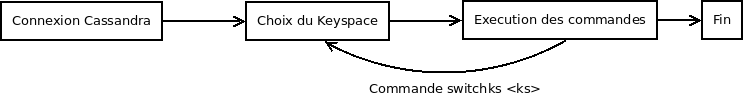
\includegraphics[width=13cm]{images/client/vie.png}
	\caption{États de l'application cliente \label{fig:vie}}
\end{figure}

\paragraph{} Le schéma~\ref{fig:vie} décrit les différents états de l'application.

\paragraph{Connexion Cassandra} Dans un premier temps, l'utilisateur doit entrer l'adresse IP à laquelle se situe la base de données Cassandra à laquelle il souhaite se connecter.
L'utilisateur a trois essais, sinon l'application se ferme. Le nombre d'essais est configurable. L'adresse entrée étant valide, 
l'objet \class{ClientApp} crée un objet \class{Cluster} initialisant la connexion à la base de données.

\paragraph{Choix du keyspace} Une fois connecté, l'utilisateur est invité à entrer le keyspace dans lequel il souhaite travailler. Si le keyspace entré n'existe pas, l'application lui propose de le créer. Il doit alors choisir une stratégie de réplication et un facteur de réplication.
L'objet \class{ClientApp} crée alors un objet \class{KeySpace} contenant les informations du keyspace et l'objet \class{Session} permettant d'envoyer des requêtes à la base de données.


\paragraph{Exécution des commandes} Le keyspace étant choisi, l'utilisateur est libre d'exécuter les commandes proposées par l'application.
\paragraph{} On distingue deux types de commandes. Les commandes permettant de consulter l'état du logiciel et de la base de données. 
C'est-à-dire, les données du keyspace courant (celui auquel nous sommes connectés), les tables stockées dans le keyspace...
\newline
\shellcmd{help}
Liste les commandes proposées par l'application accompagnée d'une brève description de chaque commande.
\shellcmd{showksdata}
Affiche les méta-données du keyspace courant : le nom du keyspace, le facteur de réplication et la stratégie de réplication utilisée.
\shellcmd{showtabledata <table>}
Affiche les méta-données de la table \texttt{<table>} : le nombre d'enregistrements, le nom des colonnes de la table et leur type.
\shellcmd{lstable}
Liste les tables stockées dans le keyspace courant.
\shellcmd{quit}
Quitte l'application cliente, on arrive donc sur l'état \textit{Fin}.

\paragraph{} Ainsi que les commandes permettant de modifier le contenu de la base de données, d'effectuer des requêtes, de modifier le keyspace courant.
\newline
\shellcmd{import <file>}
Exécute les requête au format CQL contenues dans le fichier \texttt{<file>}.
\shellcmd{switch <ks>}
Change de keyspace. Passage sur le keyspace \texttt{<ks>} avec création du keyspace s'il n'existe pas. On retourne sur l'état \textit{Choix du Keyspace}.
\shellcmd{queries <qf> <s> <ns> <nq>}
Exécute une suite de requêtes générées aléatoirement selon le seed \texttt{<s>} et la classe \texttt{<qf>}. Le nombre de simulation est définie par \texttt{<ns>} et le nombre de requêtes par simulation par \texttt{<nq>}. Cette commande est détaillée dans la partie suivante.
\shellcmd{createdatafile  <file> <nb\_tables> <nb\_rows> <data\_length>}
Écrit dans un fichier \texttt{<file>} la suite de requêtes CQL permettant de créer \texttt{<nb\_tables>} et d'insérer \texttt{<nb\_rows>} enregistrements par table. Les données crées sont de longueur \texttt{<data\_length>}.
 
\paragraph{Ajout de commandes} Une commande est une suite de caractères saisie par l'utilisateur pour exécuter une action. Elle est au format :
\shellcmd{nom\_commande <argument\_1> <argument\_2> ... <argument\_n> }
Il est aisé d'ajouter des commandes à l'application cliente.

\begin{figure}[h]
	\centering
		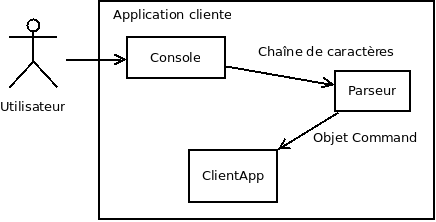
\includegraphics[width=10cm]{images/client/command.png}
	\caption{Traitement d'une commande \label{fig:commande}}
\end{figure}

\paragraph{} Un objet de type \class{Command} est la représentation d'une commande. 
Ces attributs sont l'identifiant de \texttt{nom\_comande} et un tableau de chaîne de caractères contenant tous les arguments de la commande.

\paragraph{} La commande tapée par l'utilisateur est d'abord traitée par les méthodes de la classe \class{InputCommandParser}.
Le but est de transformer la chaîne de caractères en un objet de type \class{Command}. L'objet est ensuite récupéré dans la méthode \class{run} de l'objet \class{ClientApp}
pour être exécutée par la méthode \texttt{execute} du même objet.

\paragraph{} Pour ajouter une commande, il faut donc ajouter les constantes définissant le nom de la commande, l'identifiant de la commande ainsi que son nombre d'arguments dans la classe \class{Config}.
Il faut ensuite modifier la méthode \class{whichAction} de \class{InputCommandParser} pour attribuer au nom de la commande le bon identifiant et ajouter le traitement correspondant à la commande
dans la méthode \class{execute} de \class{ClientApp}.




\subsubsection*{Problèmes et limites rencontrés}
\subsubsection*{Travail restant à réaliser}

\subsubsection{Gestion des requêtes}

\subsubsection*{Solution implémentée}
\subsubsection*{Problèmes et limites rencontrés}
\subsubsection*{Travail restant à réaliser}

\subsection{Création d'une application de visualisation de données}

\paragraph{} La visualisation des métrics de Cassandra n'étant pas une priorité du client.

\section{Tests et résultats}

\paragraph{}Pour les sections suivantes, les tests se sont déroulés sur un réseau d'Amazon composé de 10 noeuds reliés entre eux par Internet. Il faut relativiser ces résultats, car l'expérience se déroule dans des conditions idéales d'utilisation : les données sont en cache de la base de données distribuée.

\paragraph{}A noter : pour des raisons de coûts de location des machines, il ne nous a pas été possible d'effectuer plus de tests en environnement \textit{réel}, c'est à dire non simulé sur la même machine grâce à l'outil \textit{CCM}.


\subsection{Différence de temps d'exécution avec la nouvelle stratégie de placement}

\paragraph{}Pour comparer les performances de notre nouvelle stratégie de placement des données, nous allons effectuer deux tests :

\begin{itemize}
    \item On compare les temps d'exécution de différents jeux de requêtes sur un facteur de réplication de 1 (sans copie) et un facteur de 2 (avec une copie) (voir figure~\ref{fig:test_RF_PO})
    \item On réitère l'expérience avec une version de Cassandra non modifiée par nos soins (voir figure~\ref{fig:test_cassandra_non_modif_RF_PO})
\end{itemize}

\paragraph{}On remarque un gain d'environ 3 secondes sur de grands jeux de requêtes entre un facteur de réplication de 1 et de 2. On peut expliquer ce gain de performance qui est sûrement du au facteur de réplication. 

\subsection{Différence de temps d'exécution pour comparer le travail effectué sur les requêtes}

\paragraph{}Pour comparer les performances de notre traval effectué au niveau du traitement des requêtes, nous allons comparer toujours les mêmes tests (figures~\ref{fig:test_RF_PO} et~\ref{fig:test_cassandra_non_modif_RF_PO}). Pour effectuer notre analyse, nous devons étudier les courbes rouges ensembles et les bleues ensembles, afin de mettre en évidence lors d'un même facteur de réplication, le gain obtenu.

\paragraph{}La différence entre notre version et celle de Cassandra non modifiée est d'environ 1 seconde sur de grands jeux de requêtes. Les résultats sur de petits jeux de requêtes s'expliquent nottamment par un sur-coût lors des communications entre les noeuds et sur la taille des données qui est relativement petite. Les courbes de la figure~\ref{fig:test_taille_RF2} montrent d'ailleurs les différences de temps d'exécution entre une donnée de 10 Ko et de 1 Mo.


\section{Annexe - Un simulateur}

\subsection{Introduction}

\paragraph{}Derrière ce nom peu évocateur, se cache un prototype d'une base de données distribuée. Il porte le nom de simulateur car, bien évidemment, durant le temps imparti, nous n'aurions pas pu coder une base de données distribuée complète avec l'ensemble des mécanismes de traitements des données. Nous avons repris les fonctions les plus essentielles :

\begin{itemize}
    \item Le stockage des données de manière distribuée selon différentes stratégies.
    \item Le concept de distribution : Les données sont réparties et traitées par différents noeuds.
    \item La possibilité de faire des requêtes qui ont un coût de traitement.
    \item Les requêtes sont stockées sous forme de files. Il suffit de prendre la tête pour pouvoir la traiter.
    \item Un système de communication intra-noeuds.
\end{itemize}

\paragraph{}Le simulateur a pour objectif d'afficher des résultats et d'affiner la première approche des fonctions à implémenter (en particulier pour la popularité, fonction complexe à créer dans Cassandra du fait de sa distributivité).

\subsection{Etat des lieux}

\paragraph{} Le simulateur est écrit en C. Il fait environs 1300 lignes de code (commentaires Doxygen compris) pour 19 fichiers. La compilation du logiciel s'effectue dans \textit{src} en tapant la commande  : \shellcmd{make}
La compilation de la documentation Doxygen s'effectue dans \textit{data} et en tapant la commande : \shellcmd{make}

\paragraph{}Le logiciel est capable de créer des grappes de \textit{noeuds} (nommées \textit{clusters}). Il est capable de créer des \textit{requêtes}. Chaque noeud est capable de traiter des requêtes qui sont dans sa \textit{file d'exécution}. Il est possible de changer de \textit{stratégie de réplication et de positionnement} des données. Actuellement, deux stratégies ont été implémentées :

\begin{itemize}
    \item On hash l'identifiant de la donnée, on obtient un noeud et on prend les 3 suivants.
    \item Même que précédemment avec augmentation en fonction de la popularité. Les 2 objets les plus populaires sont augmentés.
\end{itemize}

\paragraph{}Le schéma de la figure~\ref{fig:archisimulateur} permet de mieux comprendre son fonctionnement. Nous allons le détailler. \newline
Tout d'abord, nous créons des données. Ensuite, nous créons des requêtes sur des données. On demande ensuite au Cluster de transmettre ces requêtes au noeud souhaité. Quand le noeud aura du temps, il traitera la requête. Si celle-ci est sur une donnée dont il a la gestion, il la traitera. Sinon, il demandera à la stratégie de lui fournir les noeuds responsables, et il transmettra.

\subsection{Inconvénients de cette approche}

\paragraph{}Premièrement, l'architecture telle qu'elle est pensée n'est pas distribuée : elle est centralisée. En effet, l'objet cluster, est un élément central du réseau. Mais dans une première approche, cela suffisait.

\paragraph{}Les noeuds sont synchrones. En effet, cette partie est omise dans la description précédente. Afin de pouvoir "simuler" totalement tous les paramètres, le cluster dispose d'une horloge appelée \textit{pas\_de\_calcul} qui consiste à donner du crédit temps à intervalle régulier aux noeuds. Les effets sont donc différents sur une base de données totalement distribuée et non synchrone que sur notre simulateur.

\subsection{Améliorations possibles}

\paragraph{}Pour obtenir un bon simulateur, il faudrait commencer par corriger les problèmes ci-dessus. Pour enlever le problème de centralisation, les noeuds devraient connaître une partie de leurs voisins, qu'il faudrait réactualiser de temps en temps. La stratégie de réplication devrait être répliquée sur tous les noeuds. Pour corriger le problème de synchronisation, et devenir asynchrone, on pourrait jouer avec un thread / noeud. Le départ serait donné par un mutex et la fin par un signal par exemple. Cependant, on perd la possiblité d'exécuter pas à pas le calcul.

\paragraph{}D'autres fonctionnalités et besoins pourraient ou devraient être implémentés : 

\begin{itemize}
    \item Possibilité de générer des requêtes sur des données aléatoires (relativement facile, créer un générateur à objets requête...)
    \item Placer les requêtes sur les noeuds de façon aléatoire (facile aussi, choisir aléatoirement les noeuds sur lequels seront poussées les requêtes dans le générateur)
    \item Travailler sur les besoins concernant les requêtes. (modification du traitement au niveau d'un noeud, moins trivial...)
\end{itemize}

\paragraph{}

\section{Conclusion et Remerciements}

TODO : C'est la fin.

\bibliography{memoire}


%%%%%%%%%%%%% BESOINS %%%%%%%%%%%%%%

\begin{figure}[H]
	\centering
		% Graphic for TeX using PGF
% Title: C:\Users\Kéké\Pictures\distribued_database.dia
% Creator: Dia v0.97.2
% CreationDate: Thu Feb 05 10:46:09 2015
% For: Kéké
% \usepackage{tikz}
% The following commands are not supported in PSTricks at present
% We define them conditionally, so when they are implemented,
% this pgf file will use them.
\ifx\du\undefined
  \newlength{\du}
\fi
\setlength{\du}{15\unitlength}
\begin{tikzpicture}
\pgftransformxscale{1.000000}
\pgftransformyscale{-1.000000}
\definecolor{dialinecolor}{rgb}{0.000000, 0.000000, 0.000000}
\pgfsetstrokecolor{dialinecolor}
\definecolor{dialinecolor}{rgb}{1.000000, 1.000000, 1.000000}
\pgfsetfillcolor{dialinecolor}
\pgfsetlinewidth{0.100000\du}
\pgfsetdash{}{0pt}
\pgfsetdash{}{0pt}
\pgfsetbuttcap
\pgfsetmiterjoin
\pgfsetlinewidth{0.100000\du}
\pgfsetbuttcap
\pgfsetmiterjoin
\pgfsetdash{}{0pt}
\definecolor{dialinecolor}{rgb}{1.000000, 1.000000, 1.000000}
\pgfsetfillcolor{dialinecolor}
\pgfpathellipse{\pgfpoint{14.237500\du}{16.387500\du}}{\pgfpoint{10.637500\du}{0\du}}{\pgfpoint{0\du}{10.637500\du}}
\pgfusepath{fill}
\definecolor{dialinecolor}{rgb}{0.000000, 0.000000, 0.000000}
\pgfsetstrokecolor{dialinecolor}
\pgfpathellipse{\pgfpoint{14.237500\du}{16.387500\du}}{\pgfpoint{10.637500\du}{0\du}}{\pgfpoint{0\du}{10.637500\du}}
\pgfusepath{stroke}
\pgfsetbuttcap
\pgfsetmiterjoin
\pgfsetdash{}{0pt}
\definecolor{dialinecolor}{rgb}{0.000000, 0.000000, 0.000000}
\pgfsetstrokecolor{dialinecolor}
\pgfpathellipse{\pgfpoint{14.237500\du}{16.387500\du}}{\pgfpoint{10.637500\du}{0\du}}{\pgfpoint{0\du}{10.637500\du}}
\pgfusepath{stroke}
\pgfsetlinewidth{0.100000\du}
\pgfsetdash{}{0pt}
\pgfsetdash{}{0pt}
\pgfsetbuttcap
\pgfsetmiterjoin
\pgfsetlinewidth{0.100000\du}
\pgfsetbuttcap
\pgfsetmiterjoin
\pgfsetdash{}{0pt}
\definecolor{dialinecolor}{rgb}{0.960784, 0.960784, 0.960784}
\pgfsetfillcolor{dialinecolor}
\pgfpathellipse{\pgfpoint{10.362500\du}{11.612500\du}}{\pgfpoint{3.562500\du}{0\du}}{\pgfpoint{0\du}{3.562500\du}}
\pgfusepath{fill}
\definecolor{dialinecolor}{rgb}{0.000000, 0.000000, 0.000000}
\pgfsetstrokecolor{dialinecolor}
\pgfpathellipse{\pgfpoint{10.362500\du}{11.612500\du}}{\pgfpoint{3.562500\du}{0\du}}{\pgfpoint{0\du}{3.562500\du}}
\pgfusepath{stroke}
\pgfsetbuttcap
\pgfsetmiterjoin
\pgfsetdash{}{0pt}
\definecolor{dialinecolor}{rgb}{0.000000, 0.000000, 0.000000}
\pgfsetstrokecolor{dialinecolor}
\pgfpathellipse{\pgfpoint{10.362500\du}{11.612500\du}}{\pgfpoint{3.562500\du}{0\du}}{\pgfpoint{0\du}{3.562500\du}}
\pgfusepath{stroke}
\pgfsetlinewidth{0.000000\du}
\pgfsetdash{}{0pt}
\pgfsetdash{}{0pt}
\pgfsetbuttcap
\pgfsetmiterjoin
\pgfsetlinewidth{0.000000\du}
\pgfsetbuttcap
\pgfsetmiterjoin
\pgfsetdash{}{0pt}
\definecolor{dialinecolor}{rgb}{0.247059, 0.317647, 0.709804}
\pgfsetfillcolor{dialinecolor}
\pgfpathellipse{\pgfpoint{10.225000\du}{8.275000\du}}{\pgfpoint{1.025000\du}{0\du}}{\pgfpoint{0\du}{1.025000\du}}
\pgfusepath{fill}
\definecolor{dialinecolor}{rgb}{0.000000, 0.000000, 0.000000}
\pgfsetstrokecolor{dialinecolor}
\pgfpathellipse{\pgfpoint{10.225000\du}{8.275000\du}}{\pgfpoint{1.025000\du}{0\du}}{\pgfpoint{0\du}{1.025000\du}}
\pgfusepath{stroke}
\pgfsetbuttcap
\pgfsetmiterjoin
\pgfsetdash{}{0pt}
\definecolor{dialinecolor}{rgb}{0.000000, 0.000000, 0.000000}
\pgfsetstrokecolor{dialinecolor}
\pgfpathellipse{\pgfpoint{10.225000\du}{8.275000\du}}{\pgfpoint{1.025000\du}{0\du}}{\pgfpoint{0\du}{1.025000\du}}
\pgfusepath{stroke}
\pgfsetlinewidth{0.000000\du}
\pgfsetdash{}{0pt}
\pgfsetdash{}{0pt}
\pgfsetbuttcap
\pgfsetmiterjoin
\pgfsetlinewidth{0.000000\du}
\pgfsetbuttcap
\pgfsetmiterjoin
\pgfsetdash{}{0pt}
\definecolor{dialinecolor}{rgb}{0.247059, 0.317647, 0.709804}
\pgfsetfillcolor{dialinecolor}
\pgfpathellipse{\pgfpoint{13.770000\du}{11.630000\du}}{\pgfpoint{1.025000\du}{0\du}}{\pgfpoint{0\du}{1.025000\du}}
\pgfusepath{fill}
\definecolor{dialinecolor}{rgb}{0.000000, 0.000000, 0.000000}
\pgfsetstrokecolor{dialinecolor}
\pgfpathellipse{\pgfpoint{13.770000\du}{11.630000\du}}{\pgfpoint{1.025000\du}{0\du}}{\pgfpoint{0\du}{1.025000\du}}
\pgfusepath{stroke}
\pgfsetbuttcap
\pgfsetmiterjoin
\pgfsetdash{}{0pt}
\definecolor{dialinecolor}{rgb}{0.000000, 0.000000, 0.000000}
\pgfsetstrokecolor{dialinecolor}
\pgfpathellipse{\pgfpoint{13.770000\du}{11.630000\du}}{\pgfpoint{1.025000\du}{0\du}}{\pgfpoint{0\du}{1.025000\du}}
\pgfusepath{stroke}
\pgfsetlinewidth{0.000000\du}
\pgfsetdash{}{0pt}
\pgfsetdash{}{0pt}
\pgfsetbuttcap
\pgfsetmiterjoin
\pgfsetlinewidth{0.000000\du}
\pgfsetbuttcap
\pgfsetmiterjoin
\pgfsetdash{}{0pt}
\definecolor{dialinecolor}{rgb}{0.247059, 0.317647, 0.709804}
\pgfsetfillcolor{dialinecolor}
\pgfpathellipse{\pgfpoint{10.265000\du}{14.985000\du}}{\pgfpoint{1.025000\du}{0\du}}{\pgfpoint{0\du}{1.025000\du}}
\pgfusepath{fill}
\definecolor{dialinecolor}{rgb}{0.000000, 0.000000, 0.000000}
\pgfsetstrokecolor{dialinecolor}
\pgfpathellipse{\pgfpoint{10.265000\du}{14.985000\du}}{\pgfpoint{1.025000\du}{0\du}}{\pgfpoint{0\du}{1.025000\du}}
\pgfusepath{stroke}
\pgfsetbuttcap
\pgfsetmiterjoin
\pgfsetdash{}{0pt}
\definecolor{dialinecolor}{rgb}{0.000000, 0.000000, 0.000000}
\pgfsetstrokecolor{dialinecolor}
\pgfpathellipse{\pgfpoint{10.265000\du}{14.985000\du}}{\pgfpoint{1.025000\du}{0\du}}{\pgfpoint{0\du}{1.025000\du}}
\pgfusepath{stroke}
\pgfsetlinewidth{0.000000\du}
\pgfsetdash{}{0pt}
\pgfsetdash{}{0pt}
\pgfsetbuttcap
\pgfsetmiterjoin
\pgfsetlinewidth{0.000000\du}
\pgfsetbuttcap
\pgfsetmiterjoin
\pgfsetdash{}{0pt}
\definecolor{dialinecolor}{rgb}{0.247059, 0.317647, 0.709804}
\pgfsetfillcolor{dialinecolor}
\pgfpathellipse{\pgfpoint{7.010000\du}{11.640000\du}}{\pgfpoint{1.025000\du}{0\du}}{\pgfpoint{0\du}{1.025000\du}}
\pgfusepath{fill}
\definecolor{dialinecolor}{rgb}{0.000000, 0.000000, 0.000000}
\pgfsetstrokecolor{dialinecolor}
\pgfpathellipse{\pgfpoint{7.010000\du}{11.640000\du}}{\pgfpoint{1.025000\du}{0\du}}{\pgfpoint{0\du}{1.025000\du}}
\pgfusepath{stroke}
\pgfsetbuttcap
\pgfsetmiterjoin
\pgfsetdash{}{0pt}
\definecolor{dialinecolor}{rgb}{0.000000, 0.000000, 0.000000}
\pgfsetstrokecolor{dialinecolor}
\pgfpathellipse{\pgfpoint{7.010000\du}{11.640000\du}}{\pgfpoint{1.025000\du}{0\du}}{\pgfpoint{0\du}{1.025000\du}}
\pgfusepath{stroke}
\pgfsetlinewidth{0.100000\du}
\pgfsetdash{}{0pt}
\pgfsetdash{}{0pt}
\pgfsetbuttcap
\pgfsetmiterjoin
\pgfsetlinewidth{0.100000\du}
\pgfsetbuttcap
\pgfsetmiterjoin
\pgfsetdash{}{0pt}
\definecolor{dialinecolor}{rgb}{0.960784, 0.960784, 0.960784}
\pgfsetfillcolor{dialinecolor}
\pgfpathellipse{\pgfpoint{18.522500\du}{13.917500\du}}{\pgfpoint{3.562500\du}{0\du}}{\pgfpoint{0\du}{3.562500\du}}
\pgfusepath{fill}
\definecolor{dialinecolor}{rgb}{0.000000, 0.000000, 0.000000}
\pgfsetstrokecolor{dialinecolor}
\pgfpathellipse{\pgfpoint{18.522500\du}{13.917500\du}}{\pgfpoint{3.562500\du}{0\du}}{\pgfpoint{0\du}{3.562500\du}}
\pgfusepath{stroke}
\pgfsetbuttcap
\pgfsetmiterjoin
\pgfsetdash{}{0pt}
\definecolor{dialinecolor}{rgb}{0.000000, 0.000000, 0.000000}
\pgfsetstrokecolor{dialinecolor}
\pgfpathellipse{\pgfpoint{18.522500\du}{13.917500\du}}{\pgfpoint{3.562500\du}{0\du}}{\pgfpoint{0\du}{3.562500\du}}
\pgfusepath{stroke}
\pgfsetlinewidth{0.000000\du}
\pgfsetdash{}{0pt}
\pgfsetdash{}{0pt}
\pgfsetbuttcap
\pgfsetmiterjoin
\pgfsetlinewidth{0.000000\du}
\pgfsetbuttcap
\pgfsetmiterjoin
\pgfsetdash{}{0pt}
\definecolor{dialinecolor}{rgb}{1.000000, 0.341176, 0.133333}
\pgfsetfillcolor{dialinecolor}
\pgfpathellipse{\pgfpoint{18.385000\du}{10.580000\du}}{\pgfpoint{1.025000\du}{0\du}}{\pgfpoint{0\du}{1.025000\du}}
\pgfusepath{fill}
\definecolor{dialinecolor}{rgb}{0.000000, 0.000000, 0.000000}
\pgfsetstrokecolor{dialinecolor}
\pgfpathellipse{\pgfpoint{18.385000\du}{10.580000\du}}{\pgfpoint{1.025000\du}{0\du}}{\pgfpoint{0\du}{1.025000\du}}
\pgfusepath{stroke}
\pgfsetbuttcap
\pgfsetmiterjoin
\pgfsetdash{}{0pt}
\definecolor{dialinecolor}{rgb}{0.000000, 0.000000, 0.000000}
\pgfsetstrokecolor{dialinecolor}
\pgfpathellipse{\pgfpoint{18.385000\du}{10.580000\du}}{\pgfpoint{1.025000\du}{0\du}}{\pgfpoint{0\du}{1.025000\du}}
\pgfusepath{stroke}
\pgfsetlinewidth{0.000000\du}
\pgfsetdash{}{0pt}
\pgfsetdash{}{0pt}
\pgfsetbuttcap
\pgfsetmiterjoin
\pgfsetlinewidth{0.000000\du}
\pgfsetbuttcap
\pgfsetmiterjoin
\pgfsetdash{}{0pt}
\definecolor{dialinecolor}{rgb}{1.000000, 0.341176, 0.133333}
\pgfsetfillcolor{dialinecolor}
\pgfpathellipse{\pgfpoint{21.930000\du}{13.935000\du}}{\pgfpoint{1.025000\du}{0\du}}{\pgfpoint{0\du}{1.025000\du}}
\pgfusepath{fill}
\definecolor{dialinecolor}{rgb}{0.000000, 0.000000, 0.000000}
\pgfsetstrokecolor{dialinecolor}
\pgfpathellipse{\pgfpoint{21.930000\du}{13.935000\du}}{\pgfpoint{1.025000\du}{0\du}}{\pgfpoint{0\du}{1.025000\du}}
\pgfusepath{stroke}
\pgfsetbuttcap
\pgfsetmiterjoin
\pgfsetdash{}{0pt}
\definecolor{dialinecolor}{rgb}{0.000000, 0.000000, 0.000000}
\pgfsetstrokecolor{dialinecolor}
\pgfpathellipse{\pgfpoint{21.930000\du}{13.935000\du}}{\pgfpoint{1.025000\du}{0\du}}{\pgfpoint{0\du}{1.025000\du}}
\pgfusepath{stroke}
\pgfsetlinewidth{0.000000\du}
\pgfsetdash{}{0pt}
\pgfsetdash{}{0pt}
\pgfsetbuttcap
\pgfsetmiterjoin
\pgfsetlinewidth{0.000000\du}
\pgfsetbuttcap
\pgfsetmiterjoin
\pgfsetdash{}{0pt}
\definecolor{dialinecolor}{rgb}{1.000000, 0.341176, 0.133333}
\pgfsetfillcolor{dialinecolor}
\pgfpathellipse{\pgfpoint{18.425000\du}{17.290000\du}}{\pgfpoint{1.025000\du}{0\du}}{\pgfpoint{0\du}{1.025000\du}}
\pgfusepath{fill}
\definecolor{dialinecolor}{rgb}{0.000000, 0.000000, 0.000000}
\pgfsetstrokecolor{dialinecolor}
\pgfpathellipse{\pgfpoint{18.425000\du}{17.290000\du}}{\pgfpoint{1.025000\du}{0\du}}{\pgfpoint{0\du}{1.025000\du}}
\pgfusepath{stroke}
\pgfsetbuttcap
\pgfsetmiterjoin
\pgfsetdash{}{0pt}
\definecolor{dialinecolor}{rgb}{0.000000, 0.000000, 0.000000}
\pgfsetstrokecolor{dialinecolor}
\pgfpathellipse{\pgfpoint{18.425000\du}{17.290000\du}}{\pgfpoint{1.025000\du}{0\du}}{\pgfpoint{0\du}{1.025000\du}}
\pgfusepath{stroke}
\pgfsetlinewidth{0.000000\du}
\pgfsetdash{}{0pt}
\pgfsetdash{}{0pt}
\pgfsetbuttcap
\pgfsetmiterjoin
\pgfsetlinewidth{0.000000\du}
\pgfsetbuttcap
\pgfsetmiterjoin
\pgfsetdash{}{0pt}
\definecolor{dialinecolor}{rgb}{1.000000, 0.341176, 0.133333}
\pgfsetfillcolor{dialinecolor}
\pgfpathellipse{\pgfpoint{15.170000\du}{13.945000\du}}{\pgfpoint{1.025000\du}{0\du}}{\pgfpoint{0\du}{1.025000\du}}
\pgfusepath{fill}
\definecolor{dialinecolor}{rgb}{0.000000, 0.000000, 0.000000}
\pgfsetstrokecolor{dialinecolor}
\pgfpathellipse{\pgfpoint{15.170000\du}{13.945000\du}}{\pgfpoint{1.025000\du}{0\du}}{\pgfpoint{0\du}{1.025000\du}}
\pgfusepath{stroke}
\pgfsetbuttcap
\pgfsetmiterjoin
\pgfsetdash{}{0pt}
\definecolor{dialinecolor}{rgb}{0.000000, 0.000000, 0.000000}
\pgfsetstrokecolor{dialinecolor}
\pgfpathellipse{\pgfpoint{15.170000\du}{13.945000\du}}{\pgfpoint{1.025000\du}{0\du}}{\pgfpoint{0\du}{1.025000\du}}
\pgfusepath{stroke}
\pgfsetlinewidth{0.100000\du}
\pgfsetdash{}{0pt}
\pgfsetdash{}{0pt}
\pgfsetbuttcap
\pgfsetmiterjoin
\pgfsetlinewidth{0.100000\du}
\pgfsetbuttcap
\pgfsetmiterjoin
\pgfsetdash{}{0pt}
\definecolor{dialinecolor}{rgb}{0.960784, 0.960784, 0.960784}
\pgfsetfillcolor{dialinecolor}
\pgfpathellipse{\pgfpoint{12.917500\du}{21.022500\du}}{\pgfpoint{3.562500\du}{0\du}}{\pgfpoint{0\du}{3.562500\du}}
\pgfusepath{fill}
\definecolor{dialinecolor}{rgb}{0.000000, 0.000000, 0.000000}
\pgfsetstrokecolor{dialinecolor}
\pgfpathellipse{\pgfpoint{12.917500\du}{21.022500\du}}{\pgfpoint{3.562500\du}{0\du}}{\pgfpoint{0\du}{3.562500\du}}
\pgfusepath{stroke}
\pgfsetbuttcap
\pgfsetmiterjoin
\pgfsetdash{}{0pt}
\definecolor{dialinecolor}{rgb}{0.000000, 0.000000, 0.000000}
\pgfsetstrokecolor{dialinecolor}
\pgfpathellipse{\pgfpoint{12.917500\du}{21.022500\du}}{\pgfpoint{3.562500\du}{0\du}}{\pgfpoint{0\du}{3.562500\du}}
\pgfusepath{stroke}
\pgfsetlinewidth{0.000000\du}
\pgfsetdash{}{0pt}
\pgfsetdash{}{0pt}
\pgfsetbuttcap
\pgfsetmiterjoin
\pgfsetlinewidth{0.000000\du}
\pgfsetbuttcap
\pgfsetmiterjoin
\pgfsetdash{}{0pt}
\definecolor{dialinecolor}{rgb}{0.298039, 0.686275, 0.313726}
\pgfsetfillcolor{dialinecolor}
\pgfpathellipse{\pgfpoint{12.780000\du}{17.685000\du}}{\pgfpoint{1.025000\du}{0\du}}{\pgfpoint{0\du}{1.025000\du}}
\pgfusepath{fill}
\definecolor{dialinecolor}{rgb}{0.000000, 0.000000, 0.000000}
\pgfsetstrokecolor{dialinecolor}
\pgfpathellipse{\pgfpoint{12.780000\du}{17.685000\du}}{\pgfpoint{1.025000\du}{0\du}}{\pgfpoint{0\du}{1.025000\du}}
\pgfusepath{stroke}
\pgfsetbuttcap
\pgfsetmiterjoin
\pgfsetdash{}{0pt}
\definecolor{dialinecolor}{rgb}{0.000000, 0.000000, 0.000000}
\pgfsetstrokecolor{dialinecolor}
\pgfpathellipse{\pgfpoint{12.780000\du}{17.685000\du}}{\pgfpoint{1.025000\du}{0\du}}{\pgfpoint{0\du}{1.025000\du}}
\pgfusepath{stroke}
\pgfsetlinewidth{0.000000\du}
\pgfsetdash{}{0pt}
\pgfsetdash{}{0pt}
\pgfsetbuttcap
\pgfsetmiterjoin
\pgfsetlinewidth{0.000000\du}
\pgfsetbuttcap
\pgfsetmiterjoin
\pgfsetdash{}{0pt}
\definecolor{dialinecolor}{rgb}{0.298039, 0.686275, 0.313726}
\pgfsetfillcolor{dialinecolor}
\pgfpathellipse{\pgfpoint{16.325000\du}{21.040000\du}}{\pgfpoint{1.025000\du}{0\du}}{\pgfpoint{0\du}{1.025000\du}}
\pgfusepath{fill}
\definecolor{dialinecolor}{rgb}{0.000000, 0.000000, 0.000000}
\pgfsetstrokecolor{dialinecolor}
\pgfpathellipse{\pgfpoint{16.325000\du}{21.040000\du}}{\pgfpoint{1.025000\du}{0\du}}{\pgfpoint{0\du}{1.025000\du}}
\pgfusepath{stroke}
\pgfsetbuttcap
\pgfsetmiterjoin
\pgfsetdash{}{0pt}
\definecolor{dialinecolor}{rgb}{0.000000, 0.000000, 0.000000}
\pgfsetstrokecolor{dialinecolor}
\pgfpathellipse{\pgfpoint{16.325000\du}{21.040000\du}}{\pgfpoint{1.025000\du}{0\du}}{\pgfpoint{0\du}{1.025000\du}}
\pgfusepath{stroke}
\pgfsetlinewidth{0.000000\du}
\pgfsetdash{}{0pt}
\pgfsetdash{}{0pt}
\pgfsetbuttcap
\pgfsetmiterjoin
\pgfsetlinewidth{0.000000\du}
\pgfsetbuttcap
\pgfsetmiterjoin
\pgfsetdash{}{0pt}
\definecolor{dialinecolor}{rgb}{0.298039, 0.686275, 0.313726}
\pgfsetfillcolor{dialinecolor}
\pgfpathellipse{\pgfpoint{12.820000\du}{24.395000\du}}{\pgfpoint{1.025000\du}{0\du}}{\pgfpoint{0\du}{1.025000\du}}
\pgfusepath{fill}
\definecolor{dialinecolor}{rgb}{0.000000, 0.000000, 0.000000}
\pgfsetstrokecolor{dialinecolor}
\pgfpathellipse{\pgfpoint{12.820000\du}{24.395000\du}}{\pgfpoint{1.025000\du}{0\du}}{\pgfpoint{0\du}{1.025000\du}}
\pgfusepath{stroke}
\pgfsetbuttcap
\pgfsetmiterjoin
\pgfsetdash{}{0pt}
\definecolor{dialinecolor}{rgb}{0.000000, 0.000000, 0.000000}
\pgfsetstrokecolor{dialinecolor}
\pgfpathellipse{\pgfpoint{12.820000\du}{24.395000\du}}{\pgfpoint{1.025000\du}{0\du}}{\pgfpoint{0\du}{1.025000\du}}
\pgfusepath{stroke}
\pgfsetlinewidth{0.000000\du}
\pgfsetdash{}{0pt}
\pgfsetdash{}{0pt}
\pgfsetbuttcap
\pgfsetmiterjoin
\pgfsetlinewidth{0.000000\du}
\pgfsetbuttcap
\pgfsetmiterjoin
\pgfsetdash{}{0pt}
\definecolor{dialinecolor}{rgb}{0.298039, 0.686275, 0.313726}
\pgfsetfillcolor{dialinecolor}
\pgfpathellipse{\pgfpoint{9.565000\du}{21.050000\du}}{\pgfpoint{1.025000\du}{0\du}}{\pgfpoint{0\du}{1.025000\du}}
\pgfusepath{fill}
\definecolor{dialinecolor}{rgb}{0.000000, 0.000000, 0.000000}
\pgfsetstrokecolor{dialinecolor}
\pgfpathellipse{\pgfpoint{9.565000\du}{21.050000\du}}{\pgfpoint{1.025000\du}{0\du}}{\pgfpoint{0\du}{1.025000\du}}
\pgfusepath{stroke}
\pgfsetbuttcap
\pgfsetmiterjoin
\pgfsetdash{}{0pt}
\definecolor{dialinecolor}{rgb}{0.000000, 0.000000, 0.000000}
\pgfsetstrokecolor{dialinecolor}
\pgfpathellipse{\pgfpoint{9.565000\du}{21.050000\du}}{\pgfpoint{1.025000\du}{0\du}}{\pgfpoint{0\du}{1.025000\du}}
\pgfusepath{stroke}
% setfont left to latex
\definecolor{dialinecolor}{rgb}{0.000000, 0.000000, 0.000000}
\pgfsetstrokecolor{dialinecolor}
\node at (10.362500\du,11.835000\du){Data Center 1};
% setfont left to latex
\definecolor{dialinecolor}{rgb}{0.000000, 0.000000, 0.000000}
\pgfsetstrokecolor{dialinecolor}
\node at (18.522500\du,14.140000\du){Data Center 2};
% setfont left to latex
\definecolor{dialinecolor}{rgb}{0.000000, 0.000000, 0.000000}
\pgfsetstrokecolor{dialinecolor}
\node at (12.917500\du,21.245000\du){Data Center 3};
% setfont left to latex
\definecolor{dialinecolor}{rgb}{0.000000, 0.000000, 0.000000}
\pgfsetstrokecolor{dialinecolor}
\node[anchor=west] at (4.687500\du,17.937500\du){Cluster};
\end{tikzpicture}

	\caption{Visualisation d'une base de données distribuée sous forme de cluster possédant trois data center\label{fig:distributed_database}}
\end{figure}

\begin{figure}[H]
	\centering
		% Graphic for TeX using PGF
% Title: C:\Users\Kéké\Pictures\Diagramme2.dia
% Creator: Dia v0.97.2
% CreationDate: Wed Feb 04 15:16:29 2015
% For: Kéké
% \usepackage{tikz}
% The following commands are not supported in PSTricks at present
% We define them conditionally, so when they are implemented,
% this pgf file will use them.
\ifx\du\undefined
  \newlength{\du}
\fi
\setlength{\du}{15\unitlength}
\begin{tikzpicture}
\pgftransformxscale{1.000000}
\pgftransformyscale{-1.000000}
\definecolor{dialinecolor}{rgb}{0.000000, 0.000000, 0.000000}
\pgfsetstrokecolor{dialinecolor}
\definecolor{dialinecolor}{rgb}{1.000000, 1.000000, 1.000000}
\pgfsetfillcolor{dialinecolor}
\pgfsetlinewidth{0.100000\du}
\pgfsetdash{}{0pt}
\pgfsetdash{}{0pt}
\pgfsetbuttcap
\pgfsetmiterjoin
\pgfsetlinewidth{0.100000\du}
\pgfsetbuttcap
\pgfsetmiterjoin
\pgfsetdash{}{0pt}
\definecolor{dialinecolor}{rgb}{0.960784, 0.960784, 0.960784}
\pgfsetfillcolor{dialinecolor}
\pgfpathellipse{\pgfpoint{12.662500\du}{-1.262500\du}}{\pgfpoint{7.462500\du}{0\du}}{\pgfpoint{0\du}{7.462500\du}}
\pgfusepath{fill}
\definecolor{dialinecolor}{rgb}{0.000000, 0.000000, 0.000000}
\pgfsetstrokecolor{dialinecolor}
\pgfpathellipse{\pgfpoint{12.662500\du}{-1.262500\du}}{\pgfpoint{7.462500\du}{0\du}}{\pgfpoint{0\du}{7.462500\du}}
\pgfusepath{stroke}
\pgfsetbuttcap
\pgfsetmiterjoin
\pgfsetdash{}{0pt}
\definecolor{dialinecolor}{rgb}{0.000000, 0.000000, 0.000000}
\pgfsetstrokecolor{dialinecolor}
\pgfpathellipse{\pgfpoint{12.662500\du}{-1.262500\du}}{\pgfpoint{7.462500\du}{0\du}}{\pgfpoint{0\du}{7.462500\du}}
\pgfusepath{stroke}
\pgfsetlinewidth{0.000000\du}
\pgfsetdash{}{0pt}
\pgfsetdash{}{0pt}
\pgfsetbuttcap
\pgfsetmiterjoin
\pgfsetlinewidth{0.000000\du}
\pgfsetbuttcap
\pgfsetmiterjoin
\pgfsetdash{}{0pt}
\definecolor{dialinecolor}{rgb}{0.247059, 0.317647, 0.709804}
\pgfsetfillcolor{dialinecolor}
\pgfpathellipse{\pgfpoint{12.737500\du}{-8.837500\du}}{\pgfpoint{1.787500\du}{0\du}}{\pgfpoint{0\du}{1.787500\du}}
\pgfusepath{fill}
\definecolor{dialinecolor}{rgb}{0.188235, 0.247059, 0.623529}
\pgfsetstrokecolor{dialinecolor}
\pgfpathellipse{\pgfpoint{12.737500\du}{-8.837500\du}}{\pgfpoint{1.787500\du}{0\du}}{\pgfpoint{0\du}{1.787500\du}}
\pgfusepath{stroke}
\pgfsetbuttcap
\pgfsetmiterjoin
\pgfsetdash{}{0pt}
\definecolor{dialinecolor}{rgb}{0.188235, 0.247059, 0.623529}
\pgfsetstrokecolor{dialinecolor}
\pgfpathellipse{\pgfpoint{12.737500\du}{-8.837500\du}}{\pgfpoint{1.787500\du}{0\du}}{\pgfpoint{0\du}{1.787500\du}}
\pgfusepath{stroke}
\pgfsetlinewidth{0.000000\du}
\pgfsetdash{}{0pt}
\pgfsetdash{}{0pt}
\pgfsetbuttcap
\pgfsetmiterjoin
\pgfsetlinewidth{0.000000\du}
\pgfsetbuttcap
\pgfsetmiterjoin
\pgfsetdash{}{0pt}
\definecolor{dialinecolor}{rgb}{0.247059, 0.317647, 0.709804}
\pgfsetfillcolor{dialinecolor}
\pgfpathellipse{\pgfpoint{20.002500\du}{-1.262500\du}}{\pgfpoint{1.787500\du}{0\du}}{\pgfpoint{0\du}{1.787500\du}}
\pgfusepath{fill}
\definecolor{dialinecolor}{rgb}{0.188235, 0.247059, 0.623529}
\pgfsetstrokecolor{dialinecolor}
\pgfpathellipse{\pgfpoint{20.002500\du}{-1.262500\du}}{\pgfpoint{1.787500\du}{0\du}}{\pgfpoint{0\du}{1.787500\du}}
\pgfusepath{stroke}
\pgfsetbuttcap
\pgfsetmiterjoin
\pgfsetdash{}{0pt}
\definecolor{dialinecolor}{rgb}{0.188235, 0.247059, 0.623529}
\pgfsetstrokecolor{dialinecolor}
\pgfpathellipse{\pgfpoint{20.002500\du}{-1.262500\du}}{\pgfpoint{1.787500\du}{0\du}}{\pgfpoint{0\du}{1.787500\du}}
\pgfusepath{stroke}
\pgfsetlinewidth{0.000000\du}
\pgfsetdash{}{0pt}
\pgfsetdash{}{0pt}
\pgfsetbuttcap
\pgfsetmiterjoin
\pgfsetlinewidth{0.000000\du}
\pgfsetbuttcap
\pgfsetmiterjoin
\pgfsetdash{}{0pt}
\definecolor{dialinecolor}{rgb}{0.247059, 0.317647, 0.709804}
\pgfsetfillcolor{dialinecolor}
\pgfpathellipse{\pgfpoint{12.667500\du}{6.212500\du}}{\pgfpoint{1.787500\du}{0\du}}{\pgfpoint{0\du}{1.787500\du}}
\pgfusepath{fill}
\definecolor{dialinecolor}{rgb}{0.188235, 0.247059, 0.623529}
\pgfsetstrokecolor{dialinecolor}
\pgfpathellipse{\pgfpoint{12.667500\du}{6.212500\du}}{\pgfpoint{1.787500\du}{0\du}}{\pgfpoint{0\du}{1.787500\du}}
\pgfusepath{stroke}
\pgfsetbuttcap
\pgfsetmiterjoin
\pgfsetdash{}{0pt}
\definecolor{dialinecolor}{rgb}{0.188235, 0.247059, 0.623529}
\pgfsetstrokecolor{dialinecolor}
\pgfpathellipse{\pgfpoint{12.667500\du}{6.212500\du}}{\pgfpoint{1.787500\du}{0\du}}{\pgfpoint{0\du}{1.787500\du}}
\pgfusepath{stroke}
\pgfsetlinewidth{0.000000\du}
\pgfsetdash{}{0pt}
\pgfsetdash{}{0pt}
\pgfsetbuttcap
\pgfsetmiterjoin
\pgfsetlinewidth{0.000000\du}
\pgfsetbuttcap
\pgfsetmiterjoin
\pgfsetdash{}{0pt}
\definecolor{dialinecolor}{rgb}{0.247059, 0.317647, 0.709804}
\pgfsetfillcolor{dialinecolor}
\pgfpathellipse{\pgfpoint{5.282500\du}{-1.312500\du}}{\pgfpoint{1.787500\du}{0\du}}{\pgfpoint{0\du}{1.787500\du}}
\pgfusepath{fill}
\definecolor{dialinecolor}{rgb}{0.188235, 0.247059, 0.623529}
\pgfsetstrokecolor{dialinecolor}
\pgfpathellipse{\pgfpoint{5.282500\du}{-1.312500\du}}{\pgfpoint{1.787500\du}{0\du}}{\pgfpoint{0\du}{1.787500\du}}
\pgfusepath{stroke}
\pgfsetbuttcap
\pgfsetmiterjoin
\pgfsetdash{}{0pt}
\definecolor{dialinecolor}{rgb}{0.188235, 0.247059, 0.623529}
\pgfsetstrokecolor{dialinecolor}
\pgfpathellipse{\pgfpoint{5.282500\du}{-1.312500\du}}{\pgfpoint{1.787500\du}{0\du}}{\pgfpoint{0\du}{1.787500\du}}
\pgfusepath{stroke}
\pgfsetlinewidth{0.100000\du}
\pgfsetdash{{\pgflinewidth}{0.200000\du}}{0cm}
\pgfsetdash{{\pgflinewidth}{0.200000\du}}{0cm}
\pgfsetbuttcap
{
\definecolor{dialinecolor}{rgb}{0.000000, 0.000000, 0.000000}
\pgfsetfillcolor{dialinecolor}
% was here!!!
\definecolor{dialinecolor}{rgb}{0.000000, 0.000000, 0.000000}
\pgfsetstrokecolor{dialinecolor}
\draw (12.737500\du,-7.050000\du)--(12.667500\du,4.425000\du);
}
\pgfsetlinewidth{0.100000\du}
\pgfsetdash{{\pgflinewidth}{0.200000\du}}{0cm}
\pgfsetdash{{\pgflinewidth}{0.200000\du}}{0cm}
\pgfsetbuttcap
{
\definecolor{dialinecolor}{rgb}{0.000000, 0.000000, 0.000000}
\pgfsetfillcolor{dialinecolor}
% was here!!!
\definecolor{dialinecolor}{rgb}{0.000000, 0.000000, 0.000000}
\pgfsetstrokecolor{dialinecolor}
\draw (7.069954\du,-1.305589\du)--(18.215000\du,-1.262500\du);
}
\pgfsetlinewidth{0.100000\du}
\pgfsetdash{}{0pt}
\pgfsetdash{}{0pt}
\pgfsetbuttcap
\pgfsetmiterjoin
\pgfsetlinewidth{0.100000\du}
\pgfsetbuttcap
\pgfsetmiterjoin
\pgfsetdash{}{0pt}
\definecolor{dialinecolor}{rgb}{1.000000, 1.000000, 1.000000}
\pgfsetfillcolor{dialinecolor}
\fill (11.682258\du,-10.925000\du)--(11.682258\du,-8.965000\du)--(13.579032\du,-8.965000\du)--(13.579032\du,-10.925000\du)--cycle;
\definecolor{dialinecolor}{rgb}{0.000000, 0.000000, 0.000000}
\pgfsetstrokecolor{dialinecolor}
\draw (11.682258\du,-10.925000\du)--(11.682258\du,-8.965000\du)--(13.579032\du,-8.965000\du)--(13.579032\du,-10.925000\du)--cycle;
\pgfsetbuttcap
\pgfsetmiterjoin
\pgfsetdash{}{0pt}
\definecolor{dialinecolor}{rgb}{0.000000, 0.000000, 0.000000}
\pgfsetstrokecolor{dialinecolor}
\draw (11.682258\du,-10.925000\du)--(11.682258\du,-8.965000\du)--(13.579032\du,-8.965000\du)--(13.579032\du,-10.925000\du)--cycle;
\pgfsetlinewidth{0.100000\du}
\pgfsetdash{}{0pt}
\pgfsetdash{}{0pt}
\pgfsetbuttcap
\pgfsetmiterjoin
\pgfsetlinewidth{0.100000\du}
\pgfsetbuttcap
\pgfsetmiterjoin
\pgfsetdash{}{0pt}
\definecolor{dialinecolor}{rgb}{1.000000, 1.000000, 1.000000}
\pgfsetfillcolor{dialinecolor}
\fill (20.015000\du,-2.300000\du)--(20.015000\du,-0.340000\du)--(21.911774\du,-0.340000\du)--(21.911774\du,-2.300000\du)--cycle;
\definecolor{dialinecolor}{rgb}{0.000000, 0.000000, 0.000000}
\pgfsetstrokecolor{dialinecolor}
\draw (20.015000\du,-2.300000\du)--(20.015000\du,-0.340000\du)--(21.911774\du,-0.340000\du)--(21.911774\du,-2.300000\du)--cycle;
\pgfsetbuttcap
\pgfsetmiterjoin
\pgfsetdash{}{0pt}
\definecolor{dialinecolor}{rgb}{0.000000, 0.000000, 0.000000}
\pgfsetstrokecolor{dialinecolor}
\draw (20.015000\du,-2.300000\du)--(20.015000\du,-0.340000\du)--(21.911774\du,-0.340000\du)--(21.911774\du,-2.300000\du)--cycle;
\pgfsetlinewidth{0.100000\du}
\pgfsetdash{}{0pt}
\pgfsetdash{}{0pt}
\pgfsetbuttcap
\pgfsetmiterjoin
\pgfsetlinewidth{0.100000\du}
\pgfsetbuttcap
\pgfsetmiterjoin
\pgfsetdash{}{0pt}
\definecolor{dialinecolor}{rgb}{1.000000, 1.000000, 1.000000}
\pgfsetfillcolor{dialinecolor}
\fill (11.730000\du,6.225000\du)--(11.730000\du,8.185000\du)--(13.626774\du,8.185000\du)--(13.626774\du,6.225000\du)--cycle;
\definecolor{dialinecolor}{rgb}{0.000000, 0.000000, 0.000000}
\pgfsetstrokecolor{dialinecolor}
\draw (11.730000\du,6.225000\du)--(11.730000\du,8.185000\du)--(13.626774\du,8.185000\du)--(13.626774\du,6.225000\du)--cycle;
\pgfsetbuttcap
\pgfsetmiterjoin
\pgfsetdash{}{0pt}
\definecolor{dialinecolor}{rgb}{0.000000, 0.000000, 0.000000}
\pgfsetstrokecolor{dialinecolor}
\draw (11.730000\du,6.225000\du)--(11.730000\du,8.185000\du)--(13.626774\du,8.185000\du)--(13.626774\du,6.225000\du)--cycle;
\pgfsetlinewidth{0.100000\du}
\pgfsetdash{}{0pt}
\pgfsetdash{}{0pt}
\pgfsetbuttcap
\pgfsetmiterjoin
\pgfsetlinewidth{0.100000\du}
\pgfsetbuttcap
\pgfsetmiterjoin
\pgfsetdash{}{0pt}
\definecolor{dialinecolor}{rgb}{1.000000, 1.000000, 1.000000}
\pgfsetfillcolor{dialinecolor}
\fill (3.545000\du,-2.300000\du)--(3.545000\du,-0.340000\du)--(5.441774\du,-0.340000\du)--(5.441774\du,-2.300000\du)--cycle;
\definecolor{dialinecolor}{rgb}{0.000000, 0.000000, 0.000000}
\pgfsetstrokecolor{dialinecolor}
\draw (3.545000\du,-2.300000\du)--(3.545000\du,-0.340000\du)--(5.441774\du,-0.340000\du)--(5.441774\du,-2.300000\du)--cycle;
\pgfsetbuttcap
\pgfsetmiterjoin
\pgfsetdash{}{0pt}
\definecolor{dialinecolor}{rgb}{0.000000, 0.000000, 0.000000}
\pgfsetstrokecolor{dialinecolor}
\draw (3.545000\du,-2.300000\du)--(3.545000\du,-0.340000\du)--(5.441774\du,-0.340000\du)--(5.441774\du,-2.300000\du)--cycle;
% setfont left to latex
\definecolor{dialinecolor}{rgb}{0.000000, 0.000000, 0.000000}
\pgfsetstrokecolor{dialinecolor}
\node at (12.630645\du,-9.652500\du){0};
% setfont left to latex
\definecolor{dialinecolor}{rgb}{0.000000, 0.000000, 0.000000}
\pgfsetstrokecolor{dialinecolor}
\node at (20.963387\du,-1.027500\du){25};
% setfont left to latex
\definecolor{dialinecolor}{rgb}{0.000000, 0.000000, 0.000000}
\pgfsetstrokecolor{dialinecolor}
\node at (12.678387\du,7.497500\du){50};
% setfont left to latex
\definecolor{dialinecolor}{rgb}{0.000000, 0.000000, 0.000000}
\pgfsetstrokecolor{dialinecolor}
\node at (4.493387\du,-1.027500\du){75};
% setfont left to latex
\definecolor{dialinecolor}{rgb}{0.000000, 0.000000, 0.000000}
\pgfsetstrokecolor{dialinecolor}
\node[anchor=west] at (5.350000\du,11.575000\du){};
% setfont left to latex
\definecolor{dialinecolor}{rgb}{0.000000, 0.000000, 0.000000}
\pgfsetstrokecolor{dialinecolor}
\node[anchor=west] at (14.700000\du,-3.725000\du){Noeud 2};
% setfont left to latex
\definecolor{dialinecolor}{rgb}{0.000000, 0.000000, 0.000000}
\pgfsetstrokecolor{dialinecolor}
\node[anchor=west] at (14.700000\du,-2.925000\du){\ensuremath{[}1,25\ensuremath{]}};
% setfont left to latex
\definecolor{dialinecolor}{rgb}{0.000000, 0.000000, 0.000000}
\pgfsetstrokecolor{dialinecolor}
\node[anchor=west] at (15.750000\du,-3.925000\du){};
% setfont left to latex
\definecolor{dialinecolor}{rgb}{0.000000, 0.000000, 0.000000}
\pgfsetstrokecolor{dialinecolor}
\node[anchor=west] at (14.500000\du,1.675000\du){Noeud 3};
% setfont left to latex
\definecolor{dialinecolor}{rgb}{0.000000, 0.000000, 0.000000}
\pgfsetstrokecolor{dialinecolor}
\node[anchor=west] at (14.500000\du,2.475000\du){\ensuremath{[}26,50\ensuremath{]}};
% setfont left to latex
\definecolor{dialinecolor}{rgb}{0.000000, 0.000000, 0.000000}
\pgfsetstrokecolor{dialinecolor}
\node[anchor=west] at (8.450000\du,1.675000\du){Noeud 4};
% setfont left to latex
\definecolor{dialinecolor}{rgb}{0.000000, 0.000000, 0.000000}
\pgfsetstrokecolor{dialinecolor}
\node[anchor=west] at (8.450000\du,2.475000\du){\ensuremath{[}51,75\ensuremath{]}};
% setfont left to latex
\definecolor{dialinecolor}{rgb}{0.000000, 0.000000, 0.000000}
\pgfsetstrokecolor{dialinecolor}
\node[anchor=west] at (8.350000\du,-3.625000\du){Noeud 1};
% setfont left to latex
\definecolor{dialinecolor}{rgb}{0.000000, 0.000000, 0.000000}
\pgfsetstrokecolor{dialinecolor}
\node[anchor=west] at (8.350000\du,-2.825000\du){\ensuremath{[}76,0\ensuremath{]}};
\pgfsetlinewidth{0.100000\du}
\pgfsetdash{}{0pt}
\pgfsetdash{}{0pt}
\pgfsetbuttcap
\pgfsetmiterjoin
\pgfsetlinewidth{0.100000\du}
\pgfsetbuttcap
\pgfsetmiterjoin
\pgfsetdash{}{0pt}
\definecolor{dialinecolor}{rgb}{1.000000, 1.000000, 1.000000}
\pgfsetfillcolor{dialinecolor}
\fill (18.082258\du,-13.525000\du)--(18.082258\du,-11.566667\du)--(19.977419\du,-11.566667\du)--(19.977419\du,-13.525000\du)--cycle;
\definecolor{dialinecolor}{rgb}{0.000000, 0.000000, 0.000000}
\pgfsetstrokecolor{dialinecolor}
\draw (18.082258\du,-13.525000\du)--(18.082258\du,-11.566667\du)--(19.977419\du,-11.566667\du)--(19.977419\du,-13.525000\du)--cycle;
\pgfsetbuttcap
\pgfsetmiterjoin
\pgfsetdash{}{0pt}
\definecolor{dialinecolor}{rgb}{0.000000, 0.000000, 0.000000}
\pgfsetstrokecolor{dialinecolor}
\draw (18.082258\du,-13.525000\du)--(18.082258\du,-11.566667\du)--(19.977419\du,-11.566667\du)--(19.977419\du,-13.525000\du)--cycle;
% setfont left to latex
\definecolor{dialinecolor}{rgb}{0.000000, 0.000000, 0.000000}
\pgfsetstrokecolor{dialinecolor}
\node at (19.029839\du,-12.253333\du){\#};
% setfont left to latex
\definecolor{dialinecolor}{rgb}{0.000000, 0.000000, 0.000000}
\pgfsetstrokecolor{dialinecolor}
\node[anchor=west] at (19.977419\du,-12.323333\du){Token};
\pgfsetlinewidth{0.000000\du}
\pgfsetdash{}{0pt}
\pgfsetdash{}{0pt}
\pgfsetbuttcap
\pgfsetmiterjoin
\pgfsetlinewidth{0.000000\du}
\pgfsetbuttcap
\pgfsetmiterjoin
\pgfsetdash{}{0pt}
\definecolor{dialinecolor}{rgb}{0.247059, 0.317647, 0.709804}
\pgfsetfillcolor{dialinecolor}
\pgfpathellipse{\pgfpoint{19.005000\du}{-9.960000\du}}{\pgfpoint{0.840000\du}{0\du}}{\pgfpoint{0\du}{0.840000\du}}
\pgfusepath{fill}
\definecolor{dialinecolor}{rgb}{0.188235, 0.247059, 0.623529}
\pgfsetstrokecolor{dialinecolor}
\pgfpathellipse{\pgfpoint{19.005000\du}{-9.960000\du}}{\pgfpoint{0.840000\du}{0\du}}{\pgfpoint{0\du}{0.840000\du}}
\pgfusepath{stroke}
\pgfsetbuttcap
\pgfsetmiterjoin
\pgfsetdash{}{0pt}
\definecolor{dialinecolor}{rgb}{0.188235, 0.247059, 0.623529}
\pgfsetstrokecolor{dialinecolor}
\pgfpathellipse{\pgfpoint{19.005000\du}{-9.960000\du}}{\pgfpoint{0.840000\du}{0\du}}{\pgfpoint{0\du}{0.840000\du}}
\pgfusepath{stroke}
% setfont left to latex
\definecolor{dialinecolor}{rgb}{0.000000, 0.000000, 0.000000}
\pgfsetstrokecolor{dialinecolor}
\node[anchor=west] at (19.845000\du,-9.737500\du){Noeud};
\end{tikzpicture}

	\caption{Exemple de partitionnement des données dans une base de données distribuée\label{fig:partitionning}}
\end{figure}

\begin{figure}[H]
	\centering
		% Graphic for TeX using PGF
% Title: C:\Users\Kéké\Pictures\multi_hash_partitionning.dia
% Creator: Dia v0.97.2
% CreationDate: Fri Feb 06 11:02:31 2015
% For: Kéké
% \usepackage{tikz}
% The following commands are not supported in PSTricks at present
% We define them conditionally, so when they are implemented,
% this pgf file will use them.
\ifx\du\undefined
  \newlength{\du}
\fi
\setlength{\du}{15\unitlength}
\begin{tikzpicture}
\pgftransformxscale{1.000000}
\pgftransformyscale{-1.000000}
\definecolor{dialinecolor}{rgb}{0.000000, 0.000000, 0.000000}
\pgfsetstrokecolor{dialinecolor}
\definecolor{dialinecolor}{rgb}{1.000000, 1.000000, 1.000000}
\pgfsetfillcolor{dialinecolor}
\pgfsetlinewidth{0.100000\du}
\pgfsetdash{}{0pt}
\pgfsetdash{}{0pt}
\pgfsetbuttcap
\pgfsetmiterjoin
\pgfsetlinewidth{0.100000\du}
\pgfsetbuttcap
\pgfsetmiterjoin
\pgfsetdash{}{0pt}
\definecolor{dialinecolor}{rgb}{0.960784, 0.960784, 0.960784}
\pgfsetfillcolor{dialinecolor}
\pgfpathellipse{\pgfpoint{12.082500\du}{15.637500\du}}{\pgfpoint{7.462500\du}{0\du}}{\pgfpoint{0\du}{7.462500\du}}
\pgfusepath{fill}
\definecolor{dialinecolor}{rgb}{0.000000, 0.000000, 0.000000}
\pgfsetstrokecolor{dialinecolor}
\pgfpathellipse{\pgfpoint{12.082500\du}{15.637500\du}}{\pgfpoint{7.462500\du}{0\du}}{\pgfpoint{0\du}{7.462500\du}}
\pgfusepath{stroke}
\pgfsetbuttcap
\pgfsetmiterjoin
\pgfsetdash{}{0pt}
\definecolor{dialinecolor}{rgb}{0.000000, 0.000000, 0.000000}
\pgfsetstrokecolor{dialinecolor}
\pgfpathellipse{\pgfpoint{12.082500\du}{15.637500\du}}{\pgfpoint{7.462500\du}{0\du}}{\pgfpoint{0\du}{7.462500\du}}
\pgfusepath{stroke}
\pgfsetlinewidth{0.000000\du}
\pgfsetdash{}{0pt}
\pgfsetdash{}{0pt}
\pgfsetbuttcap
\pgfsetmiterjoin
\pgfsetlinewidth{0.000000\du}
\pgfsetbuttcap
\pgfsetmiterjoin
\pgfsetdash{}{0pt}
\definecolor{dialinecolor}{rgb}{0.247059, 0.317647, 0.709804}
\pgfsetfillcolor{dialinecolor}
\pgfpathellipse{\pgfpoint{12.157500\du}{8.062500\du}}{\pgfpoint{1.787500\du}{0\du}}{\pgfpoint{0\du}{1.787500\du}}
\pgfusepath{fill}
\definecolor{dialinecolor}{rgb}{0.188235, 0.247059, 0.623529}
\pgfsetstrokecolor{dialinecolor}
\pgfpathellipse{\pgfpoint{12.157500\du}{8.062500\du}}{\pgfpoint{1.787500\du}{0\du}}{\pgfpoint{0\du}{1.787500\du}}
\pgfusepath{stroke}
\pgfsetbuttcap
\pgfsetmiterjoin
\pgfsetdash{}{0pt}
\definecolor{dialinecolor}{rgb}{0.188235, 0.247059, 0.623529}
\pgfsetstrokecolor{dialinecolor}
\pgfpathellipse{\pgfpoint{12.157500\du}{8.062500\du}}{\pgfpoint{1.787500\du}{0\du}}{\pgfpoint{0\du}{1.787500\du}}
\pgfusepath{stroke}
\pgfsetlinewidth{0.000000\du}
\pgfsetdash{}{0pt}
\pgfsetdash{}{0pt}
\pgfsetbuttcap
\pgfsetmiterjoin
\pgfsetlinewidth{0.000000\du}
\pgfsetbuttcap
\pgfsetmiterjoin
\pgfsetdash{}{0pt}
\definecolor{dialinecolor}{rgb}{0.247059, 0.317647, 0.709804}
\pgfsetfillcolor{dialinecolor}
\pgfpathellipse{\pgfpoint{19.422500\du}{15.637500\du}}{\pgfpoint{1.787500\du}{0\du}}{\pgfpoint{0\du}{1.787500\du}}
\pgfusepath{fill}
\definecolor{dialinecolor}{rgb}{0.188235, 0.247059, 0.623529}
\pgfsetstrokecolor{dialinecolor}
\pgfpathellipse{\pgfpoint{19.422500\du}{15.637500\du}}{\pgfpoint{1.787500\du}{0\du}}{\pgfpoint{0\du}{1.787500\du}}
\pgfusepath{stroke}
\pgfsetbuttcap
\pgfsetmiterjoin
\pgfsetdash{}{0pt}
\definecolor{dialinecolor}{rgb}{0.188235, 0.247059, 0.623529}
\pgfsetstrokecolor{dialinecolor}
\pgfpathellipse{\pgfpoint{19.422500\du}{15.637500\du}}{\pgfpoint{1.787500\du}{0\du}}{\pgfpoint{0\du}{1.787500\du}}
\pgfusepath{stroke}
\pgfsetlinewidth{0.000000\du}
\pgfsetdash{}{0pt}
\pgfsetdash{}{0pt}
\pgfsetbuttcap
\pgfsetmiterjoin
\pgfsetlinewidth{0.000000\du}
\pgfsetbuttcap
\pgfsetmiterjoin
\pgfsetdash{}{0pt}
\definecolor{dialinecolor}{rgb}{0.247059, 0.317647, 0.709804}
\pgfsetfillcolor{dialinecolor}
\pgfpathellipse{\pgfpoint{12.087500\du}{23.112500\du}}{\pgfpoint{1.787500\du}{0\du}}{\pgfpoint{0\du}{1.787500\du}}
\pgfusepath{fill}
\definecolor{dialinecolor}{rgb}{0.188235, 0.247059, 0.623529}
\pgfsetstrokecolor{dialinecolor}
\pgfpathellipse{\pgfpoint{12.087500\du}{23.112500\du}}{\pgfpoint{1.787500\du}{0\du}}{\pgfpoint{0\du}{1.787500\du}}
\pgfusepath{stroke}
\pgfsetbuttcap
\pgfsetmiterjoin
\pgfsetdash{}{0pt}
\definecolor{dialinecolor}{rgb}{0.188235, 0.247059, 0.623529}
\pgfsetstrokecolor{dialinecolor}
\pgfpathellipse{\pgfpoint{12.087500\du}{23.112500\du}}{\pgfpoint{1.787500\du}{0\du}}{\pgfpoint{0\du}{1.787500\du}}
\pgfusepath{stroke}
\pgfsetlinewidth{0.000000\du}
\pgfsetdash{}{0pt}
\pgfsetdash{}{0pt}
\pgfsetbuttcap
\pgfsetmiterjoin
\pgfsetlinewidth{0.000000\du}
\pgfsetbuttcap
\pgfsetmiterjoin
\pgfsetdash{}{0pt}
\definecolor{dialinecolor}{rgb}{0.247059, 0.317647, 0.709804}
\pgfsetfillcolor{dialinecolor}
\pgfpathellipse{\pgfpoint{4.702500\du}{15.587500\du}}{\pgfpoint{1.787500\du}{0\du}}{\pgfpoint{0\du}{1.787500\du}}
\pgfusepath{fill}
\definecolor{dialinecolor}{rgb}{0.188235, 0.247059, 0.623529}
\pgfsetstrokecolor{dialinecolor}
\pgfpathellipse{\pgfpoint{4.702500\du}{15.587500\du}}{\pgfpoint{1.787500\du}{0\du}}{\pgfpoint{0\du}{1.787500\du}}
\pgfusepath{stroke}
\pgfsetbuttcap
\pgfsetmiterjoin
\pgfsetdash{}{0pt}
\definecolor{dialinecolor}{rgb}{0.188235, 0.247059, 0.623529}
\pgfsetstrokecolor{dialinecolor}
\pgfpathellipse{\pgfpoint{4.702500\du}{15.587500\du}}{\pgfpoint{1.787500\du}{0\du}}{\pgfpoint{0\du}{1.787500\du}}
\pgfusepath{stroke}
\pgfsetlinewidth{0.100000\du}
\pgfsetdash{{\pgflinewidth}{0.200000\du}}{0cm}
\pgfsetdash{{\pgflinewidth}{0.200000\du}}{0cm}
\pgfsetbuttcap
{
\definecolor{dialinecolor}{rgb}{0.000000, 0.000000, 0.000000}
\pgfsetfillcolor{dialinecolor}
% was here!!!
\definecolor{dialinecolor}{rgb}{0.000000, 0.000000, 0.000000}
\pgfsetstrokecolor{dialinecolor}
\draw (12.157500\du,9.850000\du)--(12.087500\du,21.325000\du);
}
\pgfsetlinewidth{0.100000\du}
\pgfsetdash{{\pgflinewidth}{0.200000\du}}{0cm}
\pgfsetdash{{\pgflinewidth}{0.200000\du}}{0cm}
\pgfsetbuttcap
{
\definecolor{dialinecolor}{rgb}{0.000000, 0.000000, 0.000000}
\pgfsetfillcolor{dialinecolor}
% was here!!!
\definecolor{dialinecolor}{rgb}{0.000000, 0.000000, 0.000000}
\pgfsetstrokecolor{dialinecolor}
\draw (6.489954\du,15.594411\du)--(17.635000\du,15.637500\du);
}
\pgfsetlinewidth{0.100000\du}
\pgfsetdash{}{0pt}
\pgfsetdash{}{0pt}
\pgfsetbuttcap
\pgfsetmiterjoin
\pgfsetlinewidth{0.100000\du}
\pgfsetbuttcap
\pgfsetmiterjoin
\pgfsetdash{}{0pt}
\definecolor{dialinecolor}{rgb}{1.000000, 1.000000, 1.000000}
\pgfsetfillcolor{dialinecolor}
\fill (11.102300\du,5.975000\du)--(11.102300\du,7.935000\du)--(12.999074\du,7.935000\du)--(12.999074\du,5.975000\du)--cycle;
\definecolor{dialinecolor}{rgb}{0.000000, 0.000000, 0.000000}
\pgfsetstrokecolor{dialinecolor}
\draw (11.102300\du,5.975000\du)--(11.102300\du,7.935000\du)--(12.999074\du,7.935000\du)--(12.999074\du,5.975000\du)--cycle;
\pgfsetbuttcap
\pgfsetmiterjoin
\pgfsetdash{}{0pt}
\definecolor{dialinecolor}{rgb}{0.000000, 0.000000, 0.000000}
\pgfsetstrokecolor{dialinecolor}
\draw (11.102300\du,5.975000\du)--(11.102300\du,7.935000\du)--(12.999074\du,7.935000\du)--(12.999074\du,5.975000\du)--cycle;
\pgfsetlinewidth{0.100000\du}
\pgfsetdash{}{0pt}
\pgfsetdash{}{0pt}
\pgfsetbuttcap
\pgfsetmiterjoin
\pgfsetlinewidth{0.100000\du}
\pgfsetbuttcap
\pgfsetmiterjoin
\pgfsetdash{}{0pt}
\definecolor{dialinecolor}{rgb}{1.000000, 1.000000, 1.000000}
\pgfsetfillcolor{dialinecolor}
\fill (19.435000\du,14.600000\du)--(19.435000\du,16.560000\du)--(21.331774\du,16.560000\du)--(21.331774\du,14.600000\du)--cycle;
\definecolor{dialinecolor}{rgb}{0.000000, 0.000000, 0.000000}
\pgfsetstrokecolor{dialinecolor}
\draw (19.435000\du,14.600000\du)--(19.435000\du,16.560000\du)--(21.331774\du,16.560000\du)--(21.331774\du,14.600000\du)--cycle;
\pgfsetbuttcap
\pgfsetmiterjoin
\pgfsetdash{}{0pt}
\definecolor{dialinecolor}{rgb}{0.000000, 0.000000, 0.000000}
\pgfsetstrokecolor{dialinecolor}
\draw (19.435000\du,14.600000\du)--(19.435000\du,16.560000\du)--(21.331774\du,16.560000\du)--(21.331774\du,14.600000\du)--cycle;
\pgfsetlinewidth{0.100000\du}
\pgfsetdash{}{0pt}
\pgfsetdash{}{0pt}
\pgfsetbuttcap
\pgfsetmiterjoin
\pgfsetlinewidth{0.100000\du}
\pgfsetbuttcap
\pgfsetmiterjoin
\pgfsetdash{}{0pt}
\definecolor{dialinecolor}{rgb}{1.000000, 1.000000, 1.000000}
\pgfsetfillcolor{dialinecolor}
\fill (11.150000\du,23.125000\du)--(11.150000\du,25.085000\du)--(13.046774\du,25.085000\du)--(13.046774\du,23.125000\du)--cycle;
\definecolor{dialinecolor}{rgb}{0.000000, 0.000000, 0.000000}
\pgfsetstrokecolor{dialinecolor}
\draw (11.150000\du,23.125000\du)--(11.150000\du,25.085000\du)--(13.046774\du,25.085000\du)--(13.046774\du,23.125000\du)--cycle;
\pgfsetbuttcap
\pgfsetmiterjoin
\pgfsetdash{}{0pt}
\definecolor{dialinecolor}{rgb}{0.000000, 0.000000, 0.000000}
\pgfsetstrokecolor{dialinecolor}
\draw (11.150000\du,23.125000\du)--(11.150000\du,25.085000\du)--(13.046774\du,25.085000\du)--(13.046774\du,23.125000\du)--cycle;
\pgfsetlinewidth{0.100000\du}
\pgfsetdash{}{0pt}
\pgfsetdash{}{0pt}
\pgfsetbuttcap
\pgfsetmiterjoin
\pgfsetlinewidth{0.100000\du}
\pgfsetbuttcap
\pgfsetmiterjoin
\pgfsetdash{}{0pt}
\definecolor{dialinecolor}{rgb}{1.000000, 1.000000, 1.000000}
\pgfsetfillcolor{dialinecolor}
\fill (2.965000\du,14.600000\du)--(2.965000\du,16.560000\du)--(4.861774\du,16.560000\du)--(4.861774\du,14.600000\du)--cycle;
\definecolor{dialinecolor}{rgb}{0.000000, 0.000000, 0.000000}
\pgfsetstrokecolor{dialinecolor}
\draw (2.965000\du,14.600000\du)--(2.965000\du,16.560000\du)--(4.861774\du,16.560000\du)--(4.861774\du,14.600000\du)--cycle;
\pgfsetbuttcap
\pgfsetmiterjoin
\pgfsetdash{}{0pt}
\definecolor{dialinecolor}{rgb}{0.000000, 0.000000, 0.000000}
\pgfsetstrokecolor{dialinecolor}
\draw (2.965000\du,14.600000\du)--(2.965000\du,16.560000\du)--(4.861774\du,16.560000\du)--(4.861774\du,14.600000\du)--cycle;
% setfont left to latex
\definecolor{dialinecolor}{rgb}{0.000000, 0.000000, 0.000000}
\pgfsetstrokecolor{dialinecolor}
\node at (12.050600\du,7.247500\du){0};
% setfont left to latex
\definecolor{dialinecolor}{rgb}{0.000000, 0.000000, 0.000000}
\pgfsetstrokecolor{dialinecolor}
\node at (20.383400\du,15.872500\du){25};
% setfont left to latex
\definecolor{dialinecolor}{rgb}{0.000000, 0.000000, 0.000000}
\pgfsetstrokecolor{dialinecolor}
\node at (12.098400\du,24.397500\du){50};
% setfont left to latex
\definecolor{dialinecolor}{rgb}{0.000000, 0.000000, 0.000000}
\pgfsetstrokecolor{dialinecolor}
\node at (3.913390\du,15.872500\du){75};
% setfont left to latex
\definecolor{dialinecolor}{rgb}{0.000000, 0.000000, 0.000000}
\pgfsetstrokecolor{dialinecolor}
\node[anchor=west] at (14.120000\du,13.175000\du){Noeud 2};
% setfont left to latex
\definecolor{dialinecolor}{rgb}{0.000000, 0.000000, 0.000000}
\pgfsetstrokecolor{dialinecolor}
\node[anchor=west] at (14.120000\du,13.975000\du){\ensuremath{[}1,25\ensuremath{]}};
% setfont left to latex
\definecolor{dialinecolor}{rgb}{0.000000, 0.000000, 0.000000}
\pgfsetstrokecolor{dialinecolor}
\node[anchor=west] at (15.170000\du,12.975000\du){};
% setfont left to latex
\definecolor{dialinecolor}{rgb}{0.000000, 0.000000, 0.000000}
\pgfsetstrokecolor{dialinecolor}
\node[anchor=west] at (13.920000\du,18.575000\du){Noeud 3};
% setfont left to latex
\definecolor{dialinecolor}{rgb}{0.000000, 0.000000, 0.000000}
\pgfsetstrokecolor{dialinecolor}
\node[anchor=west] at (13.920000\du,19.375000\du){\ensuremath{[}26,50\ensuremath{]}};
% setfont left to latex
\definecolor{dialinecolor}{rgb}{0.000000, 0.000000, 0.000000}
\pgfsetstrokecolor{dialinecolor}
\node[anchor=west] at (7.870000\du,18.575000\du){Noeud 4};
% setfont left to latex
\definecolor{dialinecolor}{rgb}{0.000000, 0.000000, 0.000000}
\pgfsetstrokecolor{dialinecolor}
\node[anchor=west] at (7.870000\du,19.375000\du){\ensuremath{[}51,75\ensuremath{]}};
% setfont left to latex
\definecolor{dialinecolor}{rgb}{0.000000, 0.000000, 0.000000}
\pgfsetstrokecolor{dialinecolor}
\node[anchor=west] at (7.770000\du,13.275000\du){Noeud 1};
% setfont left to latex
\definecolor{dialinecolor}{rgb}{0.000000, 0.000000, 0.000000}
\pgfsetstrokecolor{dialinecolor}
\node[anchor=west] at (7.770000\du,14.075000\du){\ensuremath{[}76,0\ensuremath{]}};
\pgfsetlinewidth{0.000000\du}
\pgfsetdash{}{0pt}
\pgfsetdash{}{0pt}
\pgfsetbuttcap
\pgfsetmiterjoin
\pgfsetlinewidth{0.000000\du}
\pgfsetbuttcap
\pgfsetmiterjoin
\pgfsetdash{}{0pt}
\definecolor{dialinecolor}{rgb}{1.000000, 0.341176, 0.133333}
\pgfsetfillcolor{dialinecolor}
\pgfpathellipse{\pgfpoint{18.112500\du}{3.412500\du}}{\pgfpoint{0.612500\du}{0\du}}{\pgfpoint{0\du}{0.612500\du}}
\pgfusepath{fill}
\definecolor{dialinecolor}{rgb}{1.000000, 1.000000, 1.000000}
\pgfsetstrokecolor{dialinecolor}
\pgfpathellipse{\pgfpoint{18.112500\du}{3.412500\du}}{\pgfpoint{0.612500\du}{0\du}}{\pgfpoint{0\du}{0.612500\du}}
\pgfusepath{stroke}
\pgfsetbuttcap
\pgfsetmiterjoin
\pgfsetdash{}{0pt}
\definecolor{dialinecolor}{rgb}{1.000000, 1.000000, 1.000000}
\pgfsetstrokecolor{dialinecolor}
\pgfpathellipse{\pgfpoint{18.112500\du}{3.412500\du}}{\pgfpoint{0.612500\du}{0\du}}{\pgfpoint{0\du}{0.612500\du}}
\pgfusepath{stroke}
% setfont left to latex
\definecolor{dialinecolor}{rgb}{0.000000, 0.000000, 0.000000}
\pgfsetstrokecolor{dialinecolor}
\node[anchor=west] at (18.725000\du,3.635000\du){Hash1(CleObjet) = 10};
\pgfsetlinewidth{0.000000\du}
\pgfsetdash{}{0pt}
\pgfsetdash{}{0pt}
\pgfsetbuttcap
\pgfsetmiterjoin
\pgfsetlinewidth{0.000000\du}
\pgfsetbuttcap
\pgfsetmiterjoin
\pgfsetdash{}{0pt}
\definecolor{dialinecolor}{rgb}{0.298039, 0.686275, 0.313726}
\pgfsetfillcolor{dialinecolor}
\pgfpathellipse{\pgfpoint{18.077500\du}{5.387500\du}}{\pgfpoint{0.612500\du}{0\du}}{\pgfpoint{0\du}{0.612500\du}}
\pgfusepath{fill}
\definecolor{dialinecolor}{rgb}{1.000000, 1.000000, 1.000000}
\pgfsetstrokecolor{dialinecolor}
\pgfpathellipse{\pgfpoint{18.077500\du}{5.387500\du}}{\pgfpoint{0.612500\du}{0\du}}{\pgfpoint{0\du}{0.612500\du}}
\pgfusepath{stroke}
\pgfsetbuttcap
\pgfsetmiterjoin
\pgfsetdash{}{0pt}
\definecolor{dialinecolor}{rgb}{1.000000, 1.000000, 1.000000}
\pgfsetstrokecolor{dialinecolor}
\pgfpathellipse{\pgfpoint{18.077500\du}{5.387500\du}}{\pgfpoint{0.612500\du}{0\du}}{\pgfpoint{0\du}{0.612500\du}}
\pgfusepath{stroke}
% setfont left to latex
\definecolor{dialinecolor}{rgb}{0.000000, 0.000000, 0.000000}
\pgfsetstrokecolor{dialinecolor}
\node[anchor=west] at (18.690000\du,5.610000\du){Hash2(CleObjet) = 28};
\pgfsetlinewidth{0.000000\du}
\pgfsetdash{}{0pt}
\pgfsetdash{}{0pt}
\pgfsetbuttcap
\pgfsetmiterjoin
\pgfsetlinewidth{0.000000\du}
\pgfsetbuttcap
\pgfsetmiterjoin
\pgfsetdash{}{0pt}
\definecolor{dialinecolor}{rgb}{0.611765, 0.152941, 0.690196}
\pgfsetfillcolor{dialinecolor}
\pgfpathellipse{\pgfpoint{18.042500\du}{7.362500\du}}{\pgfpoint{0.612500\du}{0\du}}{\pgfpoint{0\du}{0.612500\du}}
\pgfusepath{fill}
\definecolor{dialinecolor}{rgb}{1.000000, 1.000000, 1.000000}
\pgfsetstrokecolor{dialinecolor}
\pgfpathellipse{\pgfpoint{18.042500\du}{7.362500\du}}{\pgfpoint{0.612500\du}{0\du}}{\pgfpoint{0\du}{0.612500\du}}
\pgfusepath{stroke}
\pgfsetbuttcap
\pgfsetmiterjoin
\pgfsetdash{}{0pt}
\definecolor{dialinecolor}{rgb}{1.000000, 1.000000, 1.000000}
\pgfsetstrokecolor{dialinecolor}
\pgfpathellipse{\pgfpoint{18.042500\du}{7.362500\du}}{\pgfpoint{0.612500\du}{0\du}}{\pgfpoint{0\du}{0.612500\du}}
\pgfusepath{stroke}
% setfont left to latex
\definecolor{dialinecolor}{rgb}{0.000000, 0.000000, 0.000000}
\pgfsetstrokecolor{dialinecolor}
\node[anchor=west] at (18.655000\du,7.585000\du){Hash3(CleObjet) = 88};
\pgfsetlinewidth{0.000000\du}
\pgfsetdash{}{0pt}
\pgfsetdash{}{0pt}
\pgfsetbuttcap
\pgfsetmiterjoin
\pgfsetlinewidth{0.000000\du}
\pgfsetbuttcap
\pgfsetmiterjoin
\pgfsetdash{}{0pt}
\definecolor{dialinecolor}{rgb}{1.000000, 0.341176, 0.133333}
\pgfsetfillcolor{dialinecolor}
\pgfpathellipse{\pgfpoint{15.727500\du}{9.337500\du}}{\pgfpoint{0.612500\du}{0\du}}{\pgfpoint{0\du}{0.612500\du}}
\pgfusepath{fill}
\definecolor{dialinecolor}{rgb}{1.000000, 1.000000, 1.000000}
\pgfsetstrokecolor{dialinecolor}
\pgfpathellipse{\pgfpoint{15.727500\du}{9.337500\du}}{\pgfpoint{0.612500\du}{0\du}}{\pgfpoint{0\du}{0.612500\du}}
\pgfusepath{stroke}
\pgfsetbuttcap
\pgfsetmiterjoin
\pgfsetdash{}{0pt}
\definecolor{dialinecolor}{rgb}{1.000000, 1.000000, 1.000000}
\pgfsetstrokecolor{dialinecolor}
\pgfpathellipse{\pgfpoint{15.727500\du}{9.337500\du}}{\pgfpoint{0.612500\du}{0\du}}{\pgfpoint{0\du}{0.612500\du}}
\pgfusepath{stroke}
\pgfsetlinewidth{0.000000\du}
\pgfsetdash{}{0pt}
\pgfsetdash{}{0pt}
\pgfsetbuttcap
\pgfsetmiterjoin
\pgfsetlinewidth{0.000000\du}
\pgfsetbuttcap
\pgfsetmiterjoin
\pgfsetdash{}{0pt}
\definecolor{dialinecolor}{rgb}{0.298039, 0.686275, 0.313726}
\pgfsetfillcolor{dialinecolor}
\pgfpathellipse{\pgfpoint{18.977500\du}{18.137500\du}}{\pgfpoint{0.612500\du}{0\du}}{\pgfpoint{0\du}{0.612500\du}}
\pgfusepath{fill}
\definecolor{dialinecolor}{rgb}{1.000000, 1.000000, 1.000000}
\pgfsetstrokecolor{dialinecolor}
\pgfpathellipse{\pgfpoint{18.977500\du}{18.137500\du}}{\pgfpoint{0.612500\du}{0\du}}{\pgfpoint{0\du}{0.612500\du}}
\pgfusepath{stroke}
\pgfsetbuttcap
\pgfsetmiterjoin
\pgfsetdash{}{0pt}
\definecolor{dialinecolor}{rgb}{1.000000, 1.000000, 1.000000}
\pgfsetstrokecolor{dialinecolor}
\pgfpathellipse{\pgfpoint{18.977500\du}{18.137500\du}}{\pgfpoint{0.612500\du}{0\du}}{\pgfpoint{0\du}{0.612500\du}}
\pgfusepath{stroke}
\pgfsetlinewidth{0.000000\du}
\pgfsetdash{}{0pt}
\pgfsetdash{}{0pt}
\pgfsetbuttcap
\pgfsetmiterjoin
\pgfsetlinewidth{0.000000\du}
\pgfsetbuttcap
\pgfsetmiterjoin
\pgfsetdash{}{0pt}
\definecolor{dialinecolor}{rgb}{0.611765, 0.152941, 0.690196}
\pgfsetfillcolor{dialinecolor}
\pgfpathellipse{\pgfpoint{6.327500\du}{11.087500\du}}{\pgfpoint{0.612500\du}{0\du}}{\pgfpoint{0\du}{0.612500\du}}
\pgfusepath{fill}
\definecolor{dialinecolor}{rgb}{1.000000, 1.000000, 1.000000}
\pgfsetstrokecolor{dialinecolor}
\pgfpathellipse{\pgfpoint{6.327500\du}{11.087500\du}}{\pgfpoint{0.612500\du}{0\du}}{\pgfpoint{0\du}{0.612500\du}}
\pgfusepath{stroke}
\pgfsetbuttcap
\pgfsetmiterjoin
\pgfsetdash{}{0pt}
\definecolor{dialinecolor}{rgb}{1.000000, 1.000000, 1.000000}
\pgfsetstrokecolor{dialinecolor}
\pgfpathellipse{\pgfpoint{6.327500\du}{11.087500\du}}{\pgfpoint{0.612500\du}{0\du}}{\pgfpoint{0\du}{0.612500\du}}
\pgfusepath{stroke}
% setfont left to latex
\definecolor{dialinecolor}{rgb}{0.000000, 0.000000, 0.000000}
\pgfsetstrokecolor{dialinecolor}
\node[anchor=west] at (3.100000\du,3.650000\du){Objet = \{CleObjet, Données\}};
\pgfsetlinewidth{0.100000\du}
\pgfsetdash{}{0pt}
\pgfsetdash{}{0pt}
\pgfsetbuttcap
\pgfsetmiterjoin
\pgfsetlinewidth{0.100000\du}
\pgfsetbuttcap
\pgfsetmiterjoin
\pgfsetdash{}{0pt}
\definecolor{dialinecolor}{rgb}{1.000000, 1.000000, 1.000000}
\pgfsetfillcolor{dialinecolor}
\fill (21.364919\du,20.125033\du)--(21.364919\du,22.083367\du)--(23.260081\du,22.083367\du)--(23.260081\du,20.125033\du)--cycle;
\definecolor{dialinecolor}{rgb}{0.000000, 0.000000, 0.000000}
\pgfsetstrokecolor{dialinecolor}
\draw (21.364919\du,20.125033\du)--(21.364919\du,22.083367\du)--(23.260081\du,22.083367\du)--(23.260081\du,20.125033\du)--cycle;
\pgfsetbuttcap
\pgfsetmiterjoin
\pgfsetdash{}{0pt}
\definecolor{dialinecolor}{rgb}{0.000000, 0.000000, 0.000000}
\pgfsetstrokecolor{dialinecolor}
\draw (21.364919\du,20.125033\du)--(21.364919\du,22.083367\du)--(23.260081\du,22.083367\du)--(23.260081\du,20.125033\du)--cycle;
% setfont left to latex
\definecolor{dialinecolor}{rgb}{0.000000, 0.000000, 0.000000}
\pgfsetstrokecolor{dialinecolor}
\node at (22.312500\du,21.396700\du){\#};
% setfont left to latex
\definecolor{dialinecolor}{rgb}{0.000000, 0.000000, 0.000000}
\pgfsetstrokecolor{dialinecolor}
\node[anchor=west] at (23.260081\du,21.326700\du){Token};
\pgfsetlinewidth{0.000000\du}
\pgfsetdash{}{0pt}
\pgfsetdash{}{0pt}
\pgfsetbuttcap
\pgfsetmiterjoin
\pgfsetlinewidth{0.000000\du}
\pgfsetbuttcap
\pgfsetmiterjoin
\pgfsetdash{}{0pt}
\definecolor{dialinecolor}{rgb}{0.247059, 0.317647, 0.709804}
\pgfsetfillcolor{dialinecolor}
\pgfpathellipse{\pgfpoint{22.287619\du}{23.690033\du}}{\pgfpoint{0.840000\du}{0\du}}{\pgfpoint{0\du}{0.840000\du}}
\pgfusepath{fill}
\definecolor{dialinecolor}{rgb}{0.188235, 0.247059, 0.623529}
\pgfsetstrokecolor{dialinecolor}
\pgfpathellipse{\pgfpoint{22.287619\du}{23.690033\du}}{\pgfpoint{0.840000\du}{0\du}}{\pgfpoint{0\du}{0.840000\du}}
\pgfusepath{stroke}
\pgfsetbuttcap
\pgfsetmiterjoin
\pgfsetdash{}{0pt}
\definecolor{dialinecolor}{rgb}{0.188235, 0.247059, 0.623529}
\pgfsetstrokecolor{dialinecolor}
\pgfpathellipse{\pgfpoint{22.287619\du}{23.690033\du}}{\pgfpoint{0.840000\du}{0\du}}{\pgfpoint{0\du}{0.840000\du}}
\pgfusepath{stroke}
% setfont left to latex
\definecolor{dialinecolor}{rgb}{0.000000, 0.000000, 0.000000}
\pgfsetstrokecolor{dialinecolor}
\node[anchor=west] at (23.127619\du,23.912533\du){Noeud};
\end{tikzpicture}

	\caption{Partitionnement des réplicas d'un objet avec une fonction de hachage pour chaque réplica\label{fig:multi_hash_partitionning}}
\end{figure}

\begin{figure}[H]
	\centering
		% Graphic for TeX using PGF
% Title: C:\Users\Kéké\Pictures\request.dia
% Creator: Dia v0.97.2
% CreationDate: Thu Feb 05 11:17:12 2015
% For: Kéké
% \usepackage{tikz}
% The following commands are not supported in PSTricks at present
% We define them conditionally, so when they are implemented,
% this pgf file will use them.
\ifx\du\undefined
  \newlength{\du}
\fi
\setlength{\du}{15\unitlength}
\begin{tikzpicture}
\pgftransformxscale{1.000000}
\pgftransformyscale{-1.000000}
\definecolor{dialinecolor}{rgb}{0.000000, 0.000000, 0.000000}
\pgfsetstrokecolor{dialinecolor}
\definecolor{dialinecolor}{rgb}{1.000000, 1.000000, 1.000000}
\pgfsetfillcolor{dialinecolor}
\pgfsetlinewidth{0.100000\du}
\pgfsetdash{}{0pt}
\pgfsetdash{}{0pt}
\pgfsetbuttcap
\pgfsetmiterjoin
\pgfsetlinewidth{0.100000\du}
\pgfsetbuttcap
\pgfsetmiterjoin
\pgfsetdash{}{0pt}
\definecolor{dialinecolor}{rgb}{0.960784, 0.960784, 0.960784}
\pgfsetfillcolor{dialinecolor}
\pgfpathellipse{\pgfpoint{14.750000\du}{15.250000\du}}{\pgfpoint{6.700000\du}{0\du}}{\pgfpoint{0\du}{6.700000\du}}
\pgfusepath{fill}
\definecolor{dialinecolor}{rgb}{0.000000, 0.000000, 0.000000}
\pgfsetstrokecolor{dialinecolor}
\pgfpathellipse{\pgfpoint{14.750000\du}{15.250000\du}}{\pgfpoint{6.700000\du}{0\du}}{\pgfpoint{0\du}{6.700000\du}}
\pgfusepath{stroke}
\pgfsetbuttcap
\pgfsetmiterjoin
\pgfsetdash{}{0pt}
\definecolor{dialinecolor}{rgb}{0.000000, 0.000000, 0.000000}
\pgfsetstrokecolor{dialinecolor}
\pgfpathellipse{\pgfpoint{14.750000\du}{15.250000\du}}{\pgfpoint{6.700000\du}{0\du}}{\pgfpoint{0\du}{6.700000\du}}
\pgfusepath{stroke}
\pgfsetlinewidth{0.000000\du}
\pgfsetdash{}{0pt}
\pgfsetdash{}{0pt}
\pgfsetbuttcap
\pgfsetmiterjoin
\pgfsetlinewidth{0.000000\du}
\pgfsetbuttcap
\pgfsetmiterjoin
\pgfsetdash{}{0pt}
\definecolor{dialinecolor}{rgb}{0.247059, 0.317647, 0.709804}
\pgfsetfillcolor{dialinecolor}
\pgfpathellipse{\pgfpoint{12.750000\du}{9.050000\du}}{\pgfpoint{1.300000\du}{0\du}}{\pgfpoint{0\du}{1.300000\du}}
\pgfusepath{fill}
\definecolor{dialinecolor}{rgb}{0.000000, 0.000000, 0.000000}
\pgfsetstrokecolor{dialinecolor}
\pgfpathellipse{\pgfpoint{12.750000\du}{9.050000\du}}{\pgfpoint{1.300000\du}{0\du}}{\pgfpoint{0\du}{1.300000\du}}
\pgfusepath{stroke}
\pgfsetbuttcap
\pgfsetmiterjoin
\pgfsetdash{}{0pt}
\definecolor{dialinecolor}{rgb}{0.000000, 0.000000, 0.000000}
\pgfsetstrokecolor{dialinecolor}
\pgfpathellipse{\pgfpoint{12.750000\du}{9.050000\du}}{\pgfpoint{1.300000\du}{0\du}}{\pgfpoint{0\du}{1.300000\du}}
\pgfusepath{stroke}
\pgfsetlinewidth{0.000000\du}
\pgfsetdash{}{0pt}
\pgfsetdash{}{0pt}
\pgfsetbuttcap
\pgfsetmiterjoin
\pgfsetlinewidth{0.000000\du}
\pgfsetbuttcap
\pgfsetmiterjoin
\pgfsetdash{}{0pt}
\definecolor{dialinecolor}{rgb}{0.247059, 0.317647, 0.709804}
\pgfsetfillcolor{dialinecolor}
\pgfpathellipse{\pgfpoint{16.445000\du}{8.875000\du}}{\pgfpoint{1.300000\du}{0\du}}{\pgfpoint{0\du}{1.300000\du}}
\pgfusepath{fill}
\definecolor{dialinecolor}{rgb}{0.000000, 0.000000, 0.000000}
\pgfsetstrokecolor{dialinecolor}
\pgfpathellipse{\pgfpoint{16.445000\du}{8.875000\du}}{\pgfpoint{1.300000\du}{0\du}}{\pgfpoint{0\du}{1.300000\du}}
\pgfusepath{stroke}
\pgfsetbuttcap
\pgfsetmiterjoin
\pgfsetdash{}{0pt}
\definecolor{dialinecolor}{rgb}{0.000000, 0.000000, 0.000000}
\pgfsetstrokecolor{dialinecolor}
\pgfpathellipse{\pgfpoint{16.445000\du}{8.875000\du}}{\pgfpoint{1.300000\du}{0\du}}{\pgfpoint{0\du}{1.300000\du}}
\pgfusepath{stroke}
\pgfsetlinewidth{0.000000\du}
\pgfsetdash{}{0pt}
\pgfsetdash{}{0pt}
\pgfsetbuttcap
\pgfsetmiterjoin
\pgfsetlinewidth{0.000000\du}
\pgfsetbuttcap
\pgfsetmiterjoin
\pgfsetdash{}{0pt}
\definecolor{dialinecolor}{rgb}{0.247059, 0.317647, 0.709804}
\pgfsetfillcolor{dialinecolor}
\pgfpathellipse{\pgfpoint{19.740000\du}{11.050000\du}}{\pgfpoint{1.300000\du}{0\du}}{\pgfpoint{0\du}{1.300000\du}}
\pgfusepath{fill}
\definecolor{dialinecolor}{rgb}{0.000000, 0.000000, 0.000000}
\pgfsetstrokecolor{dialinecolor}
\pgfpathellipse{\pgfpoint{19.740000\du}{11.050000\du}}{\pgfpoint{1.300000\du}{0\du}}{\pgfpoint{0\du}{1.300000\du}}
\pgfusepath{stroke}
\pgfsetbuttcap
\pgfsetmiterjoin
\pgfsetdash{}{0pt}
\definecolor{dialinecolor}{rgb}{0.000000, 0.000000, 0.000000}
\pgfsetstrokecolor{dialinecolor}
\pgfpathellipse{\pgfpoint{19.740000\du}{11.050000\du}}{\pgfpoint{1.300000\du}{0\du}}{\pgfpoint{0\du}{1.300000\du}}
\pgfusepath{stroke}
\pgfsetlinewidth{0.000000\du}
\pgfsetdash{}{0pt}
\pgfsetdash{}{0pt}
\pgfsetbuttcap
\pgfsetmiterjoin
\pgfsetlinewidth{0.000000\du}
\pgfsetbuttcap
\pgfsetmiterjoin
\pgfsetdash{}{0pt}
\definecolor{dialinecolor}{rgb}{0.247059, 0.317647, 0.709804}
\pgfsetfillcolor{dialinecolor}
\pgfpathellipse{\pgfpoint{21.235000\du}{15.425000\du}}{\pgfpoint{1.300000\du}{0\du}}{\pgfpoint{0\du}{1.300000\du}}
\pgfusepath{fill}
\definecolor{dialinecolor}{rgb}{0.000000, 0.000000, 0.000000}
\pgfsetstrokecolor{dialinecolor}
\pgfpathellipse{\pgfpoint{21.235000\du}{15.425000\du}}{\pgfpoint{1.300000\du}{0\du}}{\pgfpoint{0\du}{1.300000\du}}
\pgfusepath{stroke}
\pgfsetbuttcap
\pgfsetmiterjoin
\pgfsetdash{}{0pt}
\definecolor{dialinecolor}{rgb}{0.000000, 0.000000, 0.000000}
\pgfsetstrokecolor{dialinecolor}
\pgfpathellipse{\pgfpoint{21.235000\du}{15.425000\du}}{\pgfpoint{1.300000\du}{0\du}}{\pgfpoint{0\du}{1.300000\du}}
\pgfusepath{stroke}
\pgfsetlinewidth{0.000000\du}
\pgfsetdash{}{0pt}
\pgfsetdash{}{0pt}
\pgfsetbuttcap
\pgfsetmiterjoin
\pgfsetlinewidth{0.000000\du}
\pgfsetbuttcap
\pgfsetmiterjoin
\pgfsetdash{}{0pt}
\definecolor{dialinecolor}{rgb}{0.247059, 0.317647, 0.709804}
\pgfsetfillcolor{dialinecolor}
\pgfpathellipse{\pgfpoint{19.830000\du}{19.050000\du}}{\pgfpoint{1.300000\du}{0\du}}{\pgfpoint{0\du}{1.300000\du}}
\pgfusepath{fill}
\definecolor{dialinecolor}{rgb}{0.000000, 0.000000, 0.000000}
\pgfsetstrokecolor{dialinecolor}
\pgfpathellipse{\pgfpoint{19.830000\du}{19.050000\du}}{\pgfpoint{1.300000\du}{0\du}}{\pgfpoint{0\du}{1.300000\du}}
\pgfusepath{stroke}
\pgfsetbuttcap
\pgfsetmiterjoin
\pgfsetdash{}{0pt}
\definecolor{dialinecolor}{rgb}{0.000000, 0.000000, 0.000000}
\pgfsetstrokecolor{dialinecolor}
\pgfpathellipse{\pgfpoint{19.830000\du}{19.050000\du}}{\pgfpoint{1.300000\du}{0\du}}{\pgfpoint{0\du}{1.300000\du}}
\pgfusepath{stroke}
\pgfsetlinewidth{0.000000\du}
\pgfsetdash{}{0pt}
\pgfsetdash{}{0pt}
\pgfsetbuttcap
\pgfsetmiterjoin
\pgfsetlinewidth{0.000000\du}
\pgfsetbuttcap
\pgfsetmiterjoin
\pgfsetdash{}{0pt}
\definecolor{dialinecolor}{rgb}{0.247059, 0.317647, 0.709804}
\pgfsetfillcolor{dialinecolor}
\pgfpathellipse{\pgfpoint{16.325000\du}{21.375000\du}}{\pgfpoint{1.300000\du}{0\du}}{\pgfpoint{0\du}{1.300000\du}}
\pgfusepath{fill}
\definecolor{dialinecolor}{rgb}{0.000000, 0.000000, 0.000000}
\pgfsetstrokecolor{dialinecolor}
\pgfpathellipse{\pgfpoint{16.325000\du}{21.375000\du}}{\pgfpoint{1.300000\du}{0\du}}{\pgfpoint{0\du}{1.300000\du}}
\pgfusepath{stroke}
\pgfsetbuttcap
\pgfsetmiterjoin
\pgfsetdash{}{0pt}
\definecolor{dialinecolor}{rgb}{0.000000, 0.000000, 0.000000}
\pgfsetstrokecolor{dialinecolor}
\pgfpathellipse{\pgfpoint{16.325000\du}{21.375000\du}}{\pgfpoint{1.300000\du}{0\du}}{\pgfpoint{0\du}{1.300000\du}}
\pgfusepath{stroke}
\pgfsetlinewidth{0.000000\du}
\pgfsetdash{}{0pt}
\pgfsetdash{}{0pt}
\pgfsetbuttcap
\pgfsetmiterjoin
\pgfsetlinewidth{0.000000\du}
\pgfsetbuttcap
\pgfsetmiterjoin
\pgfsetdash{}{0pt}
\definecolor{dialinecolor}{rgb}{0.247059, 0.317647, 0.709804}
\pgfsetfillcolor{dialinecolor}
\pgfpathellipse{\pgfpoint{12.270000\du}{21.550000\du}}{\pgfpoint{1.300000\du}{0\du}}{\pgfpoint{0\du}{1.300000\du}}
\pgfusepath{fill}
\definecolor{dialinecolor}{rgb}{0.000000, 0.000000, 0.000000}
\pgfsetstrokecolor{dialinecolor}
\pgfpathellipse{\pgfpoint{12.270000\du}{21.550000\du}}{\pgfpoint{1.300000\du}{0\du}}{\pgfpoint{0\du}{1.300000\du}}
\pgfusepath{stroke}
\pgfsetbuttcap
\pgfsetmiterjoin
\pgfsetdash{}{0pt}
\definecolor{dialinecolor}{rgb}{0.000000, 0.000000, 0.000000}
\pgfsetstrokecolor{dialinecolor}
\pgfpathellipse{\pgfpoint{12.270000\du}{21.550000\du}}{\pgfpoint{1.300000\du}{0\du}}{\pgfpoint{0\du}{1.300000\du}}
\pgfusepath{stroke}
\pgfsetlinewidth{0.000000\du}
\pgfsetdash{}{0pt}
\pgfsetdash{}{0pt}
\pgfsetbuttcap
\pgfsetmiterjoin
\pgfsetlinewidth{0.000000\du}
\pgfsetbuttcap
\pgfsetmiterjoin
\pgfsetdash{}{0pt}
\definecolor{dialinecolor}{rgb}{0.247059, 0.317647, 0.709804}
\pgfsetfillcolor{dialinecolor}
\pgfpathellipse{\pgfpoint{9.265000\du}{18.975000\du}}{\pgfpoint{1.300000\du}{0\du}}{\pgfpoint{0\du}{1.300000\du}}
\pgfusepath{fill}
\definecolor{dialinecolor}{rgb}{0.000000, 0.000000, 0.000000}
\pgfsetstrokecolor{dialinecolor}
\pgfpathellipse{\pgfpoint{9.265000\du}{18.975000\du}}{\pgfpoint{1.300000\du}{0\du}}{\pgfpoint{0\du}{1.300000\du}}
\pgfusepath{stroke}
\pgfsetbuttcap
\pgfsetmiterjoin
\pgfsetdash{}{0pt}
\definecolor{dialinecolor}{rgb}{0.000000, 0.000000, 0.000000}
\pgfsetstrokecolor{dialinecolor}
\pgfpathellipse{\pgfpoint{9.265000\du}{18.975000\du}}{\pgfpoint{1.300000\du}{0\du}}{\pgfpoint{0\du}{1.300000\du}}
\pgfusepath{stroke}
\pgfsetlinewidth{0.000000\du}
\pgfsetdash{}{0pt}
\pgfsetdash{}{0pt}
\pgfsetbuttcap
\pgfsetmiterjoin
\pgfsetlinewidth{0.000000\du}
\pgfsetbuttcap
\pgfsetmiterjoin
\pgfsetdash{}{0pt}
\definecolor{dialinecolor}{rgb}{0.247059, 0.317647, 0.709804}
\pgfsetfillcolor{dialinecolor}
\pgfpathellipse{\pgfpoint{8.010000\du}{15.050000\du}}{\pgfpoint{1.300000\du}{0\du}}{\pgfpoint{0\du}{1.300000\du}}
\pgfusepath{fill}
\definecolor{dialinecolor}{rgb}{0.000000, 0.000000, 0.000000}
\pgfsetstrokecolor{dialinecolor}
\pgfpathellipse{\pgfpoint{8.010000\du}{15.050000\du}}{\pgfpoint{1.300000\du}{0\du}}{\pgfpoint{0\du}{1.300000\du}}
\pgfusepath{stroke}
\pgfsetbuttcap
\pgfsetmiterjoin
\pgfsetdash{}{0pt}
\definecolor{dialinecolor}{rgb}{0.000000, 0.000000, 0.000000}
\pgfsetstrokecolor{dialinecolor}
\pgfpathellipse{\pgfpoint{8.010000\du}{15.050000\du}}{\pgfpoint{1.300000\du}{0\du}}{\pgfpoint{0\du}{1.300000\du}}
\pgfusepath{stroke}
\pgfsetlinewidth{0.000000\du}
\pgfsetdash{}{0pt}
\pgfsetdash{}{0pt}
\pgfsetbuttcap
\pgfsetmiterjoin
\pgfsetlinewidth{0.000000\du}
\pgfsetbuttcap
\pgfsetmiterjoin
\pgfsetdash{}{0pt}
\definecolor{dialinecolor}{rgb}{0.247059, 0.317647, 0.709804}
\pgfsetfillcolor{dialinecolor}
\pgfpathellipse{\pgfpoint{9.405000\du}{11.275000\du}}{\pgfpoint{1.300000\du}{0\du}}{\pgfpoint{0\du}{1.300000\du}}
\pgfusepath{fill}
\definecolor{dialinecolor}{rgb}{0.000000, 0.000000, 0.000000}
\pgfsetstrokecolor{dialinecolor}
\pgfpathellipse{\pgfpoint{9.405000\du}{11.275000\du}}{\pgfpoint{1.300000\du}{0\du}}{\pgfpoint{0\du}{1.300000\du}}
\pgfusepath{stroke}
\pgfsetbuttcap
\pgfsetmiterjoin
\pgfsetdash{}{0pt}
\definecolor{dialinecolor}{rgb}{0.000000, 0.000000, 0.000000}
\pgfsetstrokecolor{dialinecolor}
\pgfpathellipse{\pgfpoint{9.405000\du}{11.275000\du}}{\pgfpoint{1.300000\du}{0\du}}{\pgfpoint{0\du}{1.300000\du}}
\pgfusepath{stroke}
\pgfsetlinewidth{0.100000\du}
\pgfsetdash{}{0pt}
{\pgfsetcornersarced{\pgfpoint{0.500000\du}{0.500000\du}}\definecolor{dialinecolor}{rgb}{1.000000, 1.000000, 1.000000}
\pgfsetfillcolor{dialinecolor}
\fill (3.100000\du,5.950000\du)--(3.100000\du,7.750000\du)--(7.440000\du,7.750000\du)--(7.440000\du,5.950000\du)--cycle;
}{\pgfsetcornersarced{\pgfpoint{0.500000\du}{0.500000\du}}\definecolor{dialinecolor}{rgb}{0.000000, 0.000000, 0.000000}
\pgfsetstrokecolor{dialinecolor}
\draw (3.100000\du,5.950000\du)--(3.100000\du,7.750000\du)--(7.440000\du,7.750000\du)--(7.440000\du,5.950000\du)--cycle;
}% setfont left to latex
\definecolor{dialinecolor}{rgb}{0.000000, 0.000000, 0.000000}
\pgfsetstrokecolor{dialinecolor}
\node at (5.270000\du,7.045000\du){Requête R};
\pgfsetlinewidth{0.100000\du}
\pgfsetdash{}{0pt}
\pgfsetdash{}{0pt}
\pgfsetbuttcap
{
\definecolor{dialinecolor}{rgb}{1.000000, 0.000000, 0.000000}
\pgfsetfillcolor{dialinecolor}
% was here!!!
\pgfsetarrowsend{latex}
\definecolor{dialinecolor}{rgb}{1.000000, 0.000000, 0.000000}
\pgfsetstrokecolor{dialinecolor}
\draw (6.150303\du,7.792041\du)--(8.517378\du,10.325127\du);
}
\pgfsetlinewidth{0.100000\du}
\pgfsetdash{}{0pt}
\pgfsetdash{}{0pt}
\pgfsetbuttcap
{
\definecolor{dialinecolor}{rgb}{1.000000, 0.000000, 0.000000}
\pgfsetfillcolor{dialinecolor}
% was here!!!
\pgfsetarrowsend{stealth}
\definecolor{dialinecolor}{rgb}{1.000000, 0.000000, 0.000000}
\pgfsetstrokecolor{dialinecolor}
\draw (10.704760\du,11.246703\du)--(18.440240\du,11.078297\du);
}
\pgfsetlinewidth{0.100000\du}
\pgfsetdash{}{0pt}
\pgfsetdash{}{0pt}
\pgfsetbuttcap
{
\definecolor{dialinecolor}{rgb}{1.000000, 0.000000, 0.000000}
\pgfsetfillcolor{dialinecolor}
% was here!!!
\pgfsetarrowsend{stealth}
\definecolor{dialinecolor}{rgb}{1.000000, 0.000000, 0.000000}
\pgfsetstrokecolor{dialinecolor}
\draw (10.631034\du,11.705096\du)--(20.008966\du,14.994904\du);
}
\pgfsetlinewidth{0.100000\du}
\pgfsetdash{}{0pt}
\pgfsetdash{}{0pt}
\pgfsetbuttcap
{
\definecolor{dialinecolor}{rgb}{1.000000, 0.000000, 0.000000}
\pgfsetfillcolor{dialinecolor}
% was here!!!
\pgfsetarrowsend{stealth}
\definecolor{dialinecolor}{rgb}{1.000000, 0.000000, 0.000000}
\pgfsetstrokecolor{dialinecolor}
\draw (9.405000\du,12.575000\du)--(11.756433\du,20.302345\du);
}
\pgfsetlinewidth{0.100000\du}
\pgfsetdash{}{0pt}
\pgfsetdash{}{0pt}
\pgfsetbuttcap
\pgfsetmiterjoin
\pgfsetlinewidth{0.100000\du}
\pgfsetbuttcap
\pgfsetmiterjoin
\pgfsetdash{}{0pt}
\definecolor{dialinecolor}{rgb}{1.000000, 1.000000, 1.000000}
\pgfsetfillcolor{dialinecolor}
\fill (8.850000\du,21.400000\du)--(8.850000\du,23.800000\du)--(10.500000\du,23.800000\du)--(10.500000\du,21.400000\du)--cycle;
\pgfsetbuttcap
\pgfsetmiterjoin
\pgfsetdash{}{0pt}
\definecolor{dialinecolor}{rgb}{0.000000, 0.000000, 0.000000}
\pgfsetstrokecolor{dialinecolor}
\draw (8.850000\du,21.400000\du)--(8.850000\du,23.800000\du)--(10.500000\du,23.800000\du)--(10.500000\du,21.400000\du);
\pgfsetlinewidth{0.100000\du}
\pgfsetdash{}{0pt}
\pgfsetdash{}{0pt}
\pgfsetbuttcap
{
\definecolor{dialinecolor}{rgb}{0.000000, 0.000000, 0.000000}
\pgfsetfillcolor{dialinecolor}
% was here!!!
\definecolor{dialinecolor}{rgb}{0.000000, 0.000000, 0.000000}
\pgfsetstrokecolor{dialinecolor}
\draw (8.850000\du,22.600000\du)--(10.500000\du,22.600000\du);
}
% setfont left to latex
\definecolor{dialinecolor}{rgb}{0.000000, 0.000000, 0.000000}
\pgfsetstrokecolor{dialinecolor}
\node at (9.650000\du,23.195000\du){R};
\pgfsetlinewidth{0.100000\du}
\pgfsetdash{}{0pt}
\pgfsetdash{}{0pt}
\pgfsetbuttcap
\pgfsetmiterjoin
\pgfsetlinewidth{0.100000\du}
\pgfsetbuttcap
\pgfsetmiterjoin
\pgfsetdash{}{0pt}
\definecolor{dialinecolor}{rgb}{1.000000, 1.000000, 1.000000}
\pgfsetfillcolor{dialinecolor}
\fill (20.095000\du,6.925000\du)--(20.095000\du,9.325000\du)--(21.745000\du,9.325000\du)--(21.745000\du,6.925000\du)--cycle;
\pgfsetbuttcap
\pgfsetmiterjoin
\pgfsetdash{}{0pt}
\definecolor{dialinecolor}{rgb}{0.000000, 0.000000, 0.000000}
\pgfsetstrokecolor{dialinecolor}
\draw (20.095000\du,6.925000\du)--(20.095000\du,9.325000\du)--(21.745000\du,9.325000\du)--(21.745000\du,6.925000\du);
\pgfsetlinewidth{0.100000\du}
\pgfsetdash{}{0pt}
\pgfsetdash{}{0pt}
\pgfsetbuttcap
{
\definecolor{dialinecolor}{rgb}{0.000000, 0.000000, 0.000000}
\pgfsetfillcolor{dialinecolor}
% was here!!!
\definecolor{dialinecolor}{rgb}{0.000000, 0.000000, 0.000000}
\pgfsetstrokecolor{dialinecolor}
\draw (20.095000\du,8.125000\du)--(21.745000\du,8.125000\du);
}
% setfont left to latex
\definecolor{dialinecolor}{rgb}{0.000000, 0.000000, 0.000000}
\pgfsetstrokecolor{dialinecolor}
\node at (20.895000\du,8.720000\du){R};
\pgfsetlinewidth{0.100000\du}
\pgfsetdash{}{0pt}
\pgfsetdash{}{0pt}
\pgfsetbuttcap
\pgfsetmiterjoin
\pgfsetlinewidth{0.100000\du}
\pgfsetbuttcap
\pgfsetmiterjoin
\pgfsetdash{}{0pt}
\definecolor{dialinecolor}{rgb}{1.000000, 1.000000, 1.000000}
\pgfsetfillcolor{dialinecolor}
\fill (22.840000\du,12.350000\du)--(22.840000\du,14.750000\du)--(24.490000\du,14.750000\du)--(24.490000\du,12.350000\du)--cycle;
\pgfsetbuttcap
\pgfsetmiterjoin
\pgfsetdash{}{0pt}
\definecolor{dialinecolor}{rgb}{0.000000, 0.000000, 0.000000}
\pgfsetstrokecolor{dialinecolor}
\draw (22.840000\du,12.350000\du)--(22.840000\du,14.750000\du)--(24.490000\du,14.750000\du)--(24.490000\du,12.350000\du);
\pgfsetlinewidth{0.100000\du}
\pgfsetdash{}{0pt}
\pgfsetdash{}{0pt}
\pgfsetbuttcap
{
\definecolor{dialinecolor}{rgb}{0.000000, 0.000000, 0.000000}
\pgfsetfillcolor{dialinecolor}
% was here!!!
\definecolor{dialinecolor}{rgb}{0.000000, 0.000000, 0.000000}
\pgfsetstrokecolor{dialinecolor}
\draw (22.840000\du,13.550000\du)--(24.490000\du,13.550000\du);
}
% setfont left to latex
\definecolor{dialinecolor}{rgb}{0.000000, 0.000000, 0.000000}
\pgfsetstrokecolor{dialinecolor}
\node at (23.640000\du,14.195000\du){R};
\pgfsetlinewidth{0.100000\du}
\pgfsetdash{}{0pt}
\pgfsetdash{}{0pt}
\pgfsetbuttcap
{
\definecolor{dialinecolor}{rgb}{0.298039, 0.686275, 0.313726}
\pgfsetfillcolor{dialinecolor}
% was here!!!
\pgfsetarrowsend{stealth}
\definecolor{dialinecolor}{rgb}{0.298039, 0.686275, 0.313726}
\pgfsetstrokecolor{dialinecolor}
\draw (12.270000\du,20.250000\du)--(10.016976\du,12.458150\du);
}
\pgfsetlinewidth{0.100000\du}
\pgfsetdash{}{0pt}
\pgfsetdash{}{0pt}
\pgfsetbuttcap
{
\definecolor{dialinecolor}{rgb}{0.298039, 0.686275, 0.313726}
\pgfsetfillcolor{dialinecolor}
% was here!!!
\pgfsetarrowsend{stealth}
\definecolor{dialinecolor}{rgb}{0.298039, 0.686275, 0.313726}
\pgfsetstrokecolor{dialinecolor}
\draw (9.267378\du,10.125127\du)--(6.900303\du,7.592041\du);
}
\pgfsetlinewidth{0.100000\du}
\pgfsetdash{}{0pt}
\pgfsetdash{}{0pt}
\pgfsetbuttcap
{
\definecolor{dialinecolor}{rgb}{1.000000, 0.341176, 0.133333}
\pgfsetfillcolor{dialinecolor}
% was here!!!
\pgfsetarrowsend{stealth}
\definecolor{dialinecolor}{rgb}{1.000000, 0.341176, 0.133333}
\pgfsetstrokecolor{dialinecolor}
\draw (13.343020\du,20.816899\du)--(20.161980\du,16.158101\du);
}
\pgfsetlinewidth{0.100000\du}
\pgfsetdash{}{0pt}
\pgfsetdash{}{0pt}
\pgfsetbuttcap
{
\definecolor{dialinecolor}{rgb}{1.000000, 0.341176, 0.133333}
\pgfsetfillcolor{dialinecolor}
% was here!!!
\pgfsetarrowsend{stealth}
\definecolor{dialinecolor}{rgb}{1.000000, 0.341176, 0.133333}
\pgfsetstrokecolor{dialinecolor}
\draw (13.023657\du,20.490643\du)--(18.986343\du,12.109357\du);
}
\pgfsetlinewidth{0.100000\du}
\pgfsetdash{}{0pt}
\pgfsetdash{}{0pt}
\pgfsetbuttcap
{
\definecolor{dialinecolor}{rgb}{1.000000, 0.341176, 0.133333}
\pgfsetfillcolor{dialinecolor}
% was here!!!
\definecolor{dialinecolor}{rgb}{1.000000, 0.341176, 0.133333}
\pgfsetstrokecolor{dialinecolor}
\draw (20.095000\du,8.125000\du)--(21.475000\du,9.200000\du);
}
\pgfsetlinewidth{0.100000\du}
\pgfsetdash{}{0pt}
\pgfsetdash{}{0pt}
\pgfsetbuttcap
{
\definecolor{dialinecolor}{rgb}{1.000000, 0.341176, 0.133333}
\pgfsetfillcolor{dialinecolor}
% was here!!!
\definecolor{dialinecolor}{rgb}{1.000000, 0.341176, 0.133333}
\pgfsetstrokecolor{dialinecolor}
\draw (21.520000\du,8.325000\du)--(20.225000\du,9.150000\du);
}
\pgfsetlinewidth{0.100000\du}
\pgfsetdash{}{0pt}
\pgfsetdash{}{0pt}
\pgfsetbuttcap
{
\definecolor{dialinecolor}{rgb}{1.000000, 0.341176, 0.133333}
\pgfsetfillcolor{dialinecolor}
% was here!!!
\definecolor{dialinecolor}{rgb}{1.000000, 0.341176, 0.133333}
\pgfsetstrokecolor{dialinecolor}
\draw (23.015165\du,13.595165\du)--(24.340000\du,14.600000\du);
}
\pgfsetlinewidth{0.100000\du}
\pgfsetdash{}{0pt}
\pgfsetdash{}{0pt}
\pgfsetbuttcap
{
\definecolor{dialinecolor}{rgb}{1.000000, 0.341176, 0.133333}
\pgfsetfillcolor{dialinecolor}
% was here!!!
\definecolor{dialinecolor}{rgb}{1.000000, 0.341176, 0.133333}
\pgfsetstrokecolor{dialinecolor}
\draw (24.265165\du,13.795165\du)--(23.020000\du,14.600000\du);
}
\end{tikzpicture}

	\caption{Cheminement d'une requête de lecture dans une base de données distribuée avec la prise en charge de l'affectation (un seul noeud traite la requête)\label{fig:request}}
\end{figure}

\begin{figure}[H]
	\centering
		% Graphic for TeX using PGF
% Title: C:\Users\Kéké\Pictures\write_request.dia
% Creator: Dia v0.97.2
% CreationDate: Mon Feb 23 16:23:16 2015
% For: Kéké
% \usepackage{tikz}
% The following commands are not supported in PSTricks at present
% We define them conditionally, so when they are implemented,
% this pgf file will use them.
\ifx\du\undefined
  \newlength{\du}
\fi
\setlength{\du}{15\unitlength}
\begin{tikzpicture}
\pgftransformxscale{1.000000}
\pgftransformyscale{-1.000000}
\definecolor{dialinecolor}{rgb}{0.000000, 0.000000, 0.000000}
\pgfsetstrokecolor{dialinecolor}
\definecolor{dialinecolor}{rgb}{1.000000, 1.000000, 1.000000}
\pgfsetfillcolor{dialinecolor}
\pgfsetlinewidth{0.100000\du}
\pgfsetdash{}{0pt}
\pgfsetdash{}{0pt}
\pgfsetbuttcap
\pgfsetmiterjoin
\pgfsetlinewidth{0.100000\du}
\pgfsetbuttcap
\pgfsetmiterjoin
\pgfsetdash{}{0pt}
\definecolor{dialinecolor}{rgb}{0.960784, 0.960784, 0.960784}
\pgfsetfillcolor{dialinecolor}
\pgfpathellipse{\pgfpoint{14.695000\du}{15.730200\du}}{\pgfpoint{6.700000\du}{0\du}}{\pgfpoint{0\du}{6.700000\du}}
\pgfusepath{fill}
\definecolor{dialinecolor}{rgb}{0.000000, 0.000000, 0.000000}
\pgfsetstrokecolor{dialinecolor}
\pgfpathellipse{\pgfpoint{14.695000\du}{15.730200\du}}{\pgfpoint{6.700000\du}{0\du}}{\pgfpoint{0\du}{6.700000\du}}
\pgfusepath{stroke}
\pgfsetbuttcap
\pgfsetmiterjoin
\pgfsetdash{}{0pt}
\definecolor{dialinecolor}{rgb}{0.000000, 0.000000, 0.000000}
\pgfsetstrokecolor{dialinecolor}
\pgfpathellipse{\pgfpoint{14.695000\du}{15.730200\du}}{\pgfpoint{6.700000\du}{0\du}}{\pgfpoint{0\du}{6.700000\du}}
\pgfusepath{stroke}
\pgfsetlinewidth{0.000000\du}
\pgfsetdash{}{0pt}
\pgfsetdash{}{0pt}
\pgfsetbuttcap
\pgfsetmiterjoin
\pgfsetlinewidth{0.000000\du}
\pgfsetbuttcap
\pgfsetmiterjoin
\pgfsetdash{}{0pt}
\definecolor{dialinecolor}{rgb}{0.247059, 0.317647, 0.709804}
\pgfsetfillcolor{dialinecolor}
\pgfpathellipse{\pgfpoint{12.695000\du}{9.530200\du}}{\pgfpoint{1.300000\du}{0\du}}{\pgfpoint{0\du}{1.300000\du}}
\pgfusepath{fill}
\definecolor{dialinecolor}{rgb}{0.000000, 0.000000, 0.000000}
\pgfsetstrokecolor{dialinecolor}
\pgfpathellipse{\pgfpoint{12.695000\du}{9.530200\du}}{\pgfpoint{1.300000\du}{0\du}}{\pgfpoint{0\du}{1.300000\du}}
\pgfusepath{stroke}
\pgfsetbuttcap
\pgfsetmiterjoin
\pgfsetdash{}{0pt}
\definecolor{dialinecolor}{rgb}{0.000000, 0.000000, 0.000000}
\pgfsetstrokecolor{dialinecolor}
\pgfpathellipse{\pgfpoint{12.695000\du}{9.530200\du}}{\pgfpoint{1.300000\du}{0\du}}{\pgfpoint{0\du}{1.300000\du}}
\pgfusepath{stroke}
\pgfsetlinewidth{0.000000\du}
\pgfsetdash{}{0pt}
\pgfsetdash{}{0pt}
\pgfsetbuttcap
\pgfsetmiterjoin
\pgfsetlinewidth{0.000000\du}
\pgfsetbuttcap
\pgfsetmiterjoin
\pgfsetdash{}{0pt}
\definecolor{dialinecolor}{rgb}{0.247059, 0.317647, 0.709804}
\pgfsetfillcolor{dialinecolor}
\pgfpathellipse{\pgfpoint{16.390000\du}{9.355200\du}}{\pgfpoint{1.300000\du}{0\du}}{\pgfpoint{0\du}{1.300000\du}}
\pgfusepath{fill}
\definecolor{dialinecolor}{rgb}{0.000000, 0.000000, 0.000000}
\pgfsetstrokecolor{dialinecolor}
\pgfpathellipse{\pgfpoint{16.390000\du}{9.355200\du}}{\pgfpoint{1.300000\du}{0\du}}{\pgfpoint{0\du}{1.300000\du}}
\pgfusepath{stroke}
\pgfsetbuttcap
\pgfsetmiterjoin
\pgfsetdash{}{0pt}
\definecolor{dialinecolor}{rgb}{0.000000, 0.000000, 0.000000}
\pgfsetstrokecolor{dialinecolor}
\pgfpathellipse{\pgfpoint{16.390000\du}{9.355200\du}}{\pgfpoint{1.300000\du}{0\du}}{\pgfpoint{0\du}{1.300000\du}}
\pgfusepath{stroke}
\pgfsetlinewidth{0.000000\du}
\pgfsetdash{}{0pt}
\pgfsetdash{}{0pt}
\pgfsetbuttcap
\pgfsetmiterjoin
\pgfsetlinewidth{0.000000\du}
\pgfsetbuttcap
\pgfsetmiterjoin
\pgfsetdash{}{0pt}
\definecolor{dialinecolor}{rgb}{0.247059, 0.317647, 0.709804}
\pgfsetfillcolor{dialinecolor}
\pgfpathellipse{\pgfpoint{19.685000\du}{11.530200\du}}{\pgfpoint{1.300000\du}{0\du}}{\pgfpoint{0\du}{1.300000\du}}
\pgfusepath{fill}
\definecolor{dialinecolor}{rgb}{0.000000, 0.000000, 0.000000}
\pgfsetstrokecolor{dialinecolor}
\pgfpathellipse{\pgfpoint{19.685000\du}{11.530200\du}}{\pgfpoint{1.300000\du}{0\du}}{\pgfpoint{0\du}{1.300000\du}}
\pgfusepath{stroke}
\pgfsetbuttcap
\pgfsetmiterjoin
\pgfsetdash{}{0pt}
\definecolor{dialinecolor}{rgb}{0.000000, 0.000000, 0.000000}
\pgfsetstrokecolor{dialinecolor}
\pgfpathellipse{\pgfpoint{19.685000\du}{11.530200\du}}{\pgfpoint{1.300000\du}{0\du}}{\pgfpoint{0\du}{1.300000\du}}
\pgfusepath{stroke}
\pgfsetlinewidth{0.000000\du}
\pgfsetdash{}{0pt}
\pgfsetdash{}{0pt}
\pgfsetbuttcap
\pgfsetmiterjoin
\pgfsetlinewidth{0.000000\du}
\pgfsetbuttcap
\pgfsetmiterjoin
\pgfsetdash{}{0pt}
\definecolor{dialinecolor}{rgb}{0.247059, 0.317647, 0.709804}
\pgfsetfillcolor{dialinecolor}
\pgfpathellipse{\pgfpoint{21.180000\du}{15.905200\du}}{\pgfpoint{1.300000\du}{0\du}}{\pgfpoint{0\du}{1.300000\du}}
\pgfusepath{fill}
\definecolor{dialinecolor}{rgb}{0.000000, 0.000000, 0.000000}
\pgfsetstrokecolor{dialinecolor}
\pgfpathellipse{\pgfpoint{21.180000\du}{15.905200\du}}{\pgfpoint{1.300000\du}{0\du}}{\pgfpoint{0\du}{1.300000\du}}
\pgfusepath{stroke}
\pgfsetbuttcap
\pgfsetmiterjoin
\pgfsetdash{}{0pt}
\definecolor{dialinecolor}{rgb}{0.000000, 0.000000, 0.000000}
\pgfsetstrokecolor{dialinecolor}
\pgfpathellipse{\pgfpoint{21.180000\du}{15.905200\du}}{\pgfpoint{1.300000\du}{0\du}}{\pgfpoint{0\du}{1.300000\du}}
\pgfusepath{stroke}
\pgfsetlinewidth{0.000000\du}
\pgfsetdash{}{0pt}
\pgfsetdash{}{0pt}
\pgfsetbuttcap
\pgfsetmiterjoin
\pgfsetlinewidth{0.000000\du}
\pgfsetbuttcap
\pgfsetmiterjoin
\pgfsetdash{}{0pt}
\definecolor{dialinecolor}{rgb}{0.247059, 0.317647, 0.709804}
\pgfsetfillcolor{dialinecolor}
\pgfpathellipse{\pgfpoint{19.775000\du}{19.530200\du}}{\pgfpoint{1.300000\du}{0\du}}{\pgfpoint{0\du}{1.300000\du}}
\pgfusepath{fill}
\definecolor{dialinecolor}{rgb}{0.000000, 0.000000, 0.000000}
\pgfsetstrokecolor{dialinecolor}
\pgfpathellipse{\pgfpoint{19.775000\du}{19.530200\du}}{\pgfpoint{1.300000\du}{0\du}}{\pgfpoint{0\du}{1.300000\du}}
\pgfusepath{stroke}
\pgfsetbuttcap
\pgfsetmiterjoin
\pgfsetdash{}{0pt}
\definecolor{dialinecolor}{rgb}{0.000000, 0.000000, 0.000000}
\pgfsetstrokecolor{dialinecolor}
\pgfpathellipse{\pgfpoint{19.775000\du}{19.530200\du}}{\pgfpoint{1.300000\du}{0\du}}{\pgfpoint{0\du}{1.300000\du}}
\pgfusepath{stroke}
\pgfsetlinewidth{0.000000\du}
\pgfsetdash{}{0pt}
\pgfsetdash{}{0pt}
\pgfsetbuttcap
\pgfsetmiterjoin
\pgfsetlinewidth{0.000000\du}
\pgfsetbuttcap
\pgfsetmiterjoin
\pgfsetdash{}{0pt}
\definecolor{dialinecolor}{rgb}{0.247059, 0.317647, 0.709804}
\pgfsetfillcolor{dialinecolor}
\pgfpathellipse{\pgfpoint{16.270000\du}{21.855200\du}}{\pgfpoint{1.300000\du}{0\du}}{\pgfpoint{0\du}{1.300000\du}}
\pgfusepath{fill}
\definecolor{dialinecolor}{rgb}{0.000000, 0.000000, 0.000000}
\pgfsetstrokecolor{dialinecolor}
\pgfpathellipse{\pgfpoint{16.270000\du}{21.855200\du}}{\pgfpoint{1.300000\du}{0\du}}{\pgfpoint{0\du}{1.300000\du}}
\pgfusepath{stroke}
\pgfsetbuttcap
\pgfsetmiterjoin
\pgfsetdash{}{0pt}
\definecolor{dialinecolor}{rgb}{0.000000, 0.000000, 0.000000}
\pgfsetstrokecolor{dialinecolor}
\pgfpathellipse{\pgfpoint{16.270000\du}{21.855200\du}}{\pgfpoint{1.300000\du}{0\du}}{\pgfpoint{0\du}{1.300000\du}}
\pgfusepath{stroke}
\pgfsetlinewidth{0.000000\du}
\pgfsetdash{}{0pt}
\pgfsetdash{}{0pt}
\pgfsetbuttcap
\pgfsetmiterjoin
\pgfsetlinewidth{0.000000\du}
\pgfsetbuttcap
\pgfsetmiterjoin
\pgfsetdash{}{0pt}
\definecolor{dialinecolor}{rgb}{0.247059, 0.317647, 0.709804}
\pgfsetfillcolor{dialinecolor}
\pgfpathellipse{\pgfpoint{12.215000\du}{22.030200\du}}{\pgfpoint{1.300000\du}{0\du}}{\pgfpoint{0\du}{1.300000\du}}
\pgfusepath{fill}
\definecolor{dialinecolor}{rgb}{0.000000, 0.000000, 0.000000}
\pgfsetstrokecolor{dialinecolor}
\pgfpathellipse{\pgfpoint{12.215000\du}{22.030200\du}}{\pgfpoint{1.300000\du}{0\du}}{\pgfpoint{0\du}{1.300000\du}}
\pgfusepath{stroke}
\pgfsetbuttcap
\pgfsetmiterjoin
\pgfsetdash{}{0pt}
\definecolor{dialinecolor}{rgb}{0.000000, 0.000000, 0.000000}
\pgfsetstrokecolor{dialinecolor}
\pgfpathellipse{\pgfpoint{12.215000\du}{22.030200\du}}{\pgfpoint{1.300000\du}{0\du}}{\pgfpoint{0\du}{1.300000\du}}
\pgfusepath{stroke}
\pgfsetlinewidth{0.000000\du}
\pgfsetdash{}{0pt}
\pgfsetdash{}{0pt}
\pgfsetbuttcap
\pgfsetmiterjoin
\pgfsetlinewidth{0.000000\du}
\pgfsetbuttcap
\pgfsetmiterjoin
\pgfsetdash{}{0pt}
\definecolor{dialinecolor}{rgb}{0.247059, 0.317647, 0.709804}
\pgfsetfillcolor{dialinecolor}
\pgfpathellipse{\pgfpoint{9.210000\du}{19.455200\du}}{\pgfpoint{1.300000\du}{0\du}}{\pgfpoint{0\du}{1.300000\du}}
\pgfusepath{fill}
\definecolor{dialinecolor}{rgb}{0.000000, 0.000000, 0.000000}
\pgfsetstrokecolor{dialinecolor}
\pgfpathellipse{\pgfpoint{9.210000\du}{19.455200\du}}{\pgfpoint{1.300000\du}{0\du}}{\pgfpoint{0\du}{1.300000\du}}
\pgfusepath{stroke}
\pgfsetbuttcap
\pgfsetmiterjoin
\pgfsetdash{}{0pt}
\definecolor{dialinecolor}{rgb}{0.000000, 0.000000, 0.000000}
\pgfsetstrokecolor{dialinecolor}
\pgfpathellipse{\pgfpoint{9.210000\du}{19.455200\du}}{\pgfpoint{1.300000\du}{0\du}}{\pgfpoint{0\du}{1.300000\du}}
\pgfusepath{stroke}
\pgfsetlinewidth{0.000000\du}
\pgfsetdash{}{0pt}
\pgfsetdash{}{0pt}
\pgfsetbuttcap
\pgfsetmiterjoin
\pgfsetlinewidth{0.000000\du}
\pgfsetbuttcap
\pgfsetmiterjoin
\pgfsetdash{}{0pt}
\definecolor{dialinecolor}{rgb}{0.247059, 0.317647, 0.709804}
\pgfsetfillcolor{dialinecolor}
\pgfpathellipse{\pgfpoint{7.955000\du}{15.530200\du}}{\pgfpoint{1.300000\du}{0\du}}{\pgfpoint{0\du}{1.300000\du}}
\pgfusepath{fill}
\definecolor{dialinecolor}{rgb}{0.000000, 0.000000, 0.000000}
\pgfsetstrokecolor{dialinecolor}
\pgfpathellipse{\pgfpoint{7.955000\du}{15.530200\du}}{\pgfpoint{1.300000\du}{0\du}}{\pgfpoint{0\du}{1.300000\du}}
\pgfusepath{stroke}
\pgfsetbuttcap
\pgfsetmiterjoin
\pgfsetdash{}{0pt}
\definecolor{dialinecolor}{rgb}{0.000000, 0.000000, 0.000000}
\pgfsetstrokecolor{dialinecolor}
\pgfpathellipse{\pgfpoint{7.955000\du}{15.530200\du}}{\pgfpoint{1.300000\du}{0\du}}{\pgfpoint{0\du}{1.300000\du}}
\pgfusepath{stroke}
\pgfsetlinewidth{0.000000\du}
\pgfsetdash{}{0pt}
\pgfsetdash{}{0pt}
\pgfsetbuttcap
\pgfsetmiterjoin
\pgfsetlinewidth{0.000000\du}
\pgfsetbuttcap
\pgfsetmiterjoin
\pgfsetdash{}{0pt}
\definecolor{dialinecolor}{rgb}{0.247059, 0.317647, 0.709804}
\pgfsetfillcolor{dialinecolor}
\pgfpathellipse{\pgfpoint{9.350000\du}{11.755200\du}}{\pgfpoint{1.300000\du}{0\du}}{\pgfpoint{0\du}{1.300000\du}}
\pgfusepath{fill}
\definecolor{dialinecolor}{rgb}{0.000000, 0.000000, 0.000000}
\pgfsetstrokecolor{dialinecolor}
\pgfpathellipse{\pgfpoint{9.350000\du}{11.755200\du}}{\pgfpoint{1.300000\du}{0\du}}{\pgfpoint{0\du}{1.300000\du}}
\pgfusepath{stroke}
\pgfsetbuttcap
\pgfsetmiterjoin
\pgfsetdash{}{0pt}
\definecolor{dialinecolor}{rgb}{0.000000, 0.000000, 0.000000}
\pgfsetstrokecolor{dialinecolor}
\pgfpathellipse{\pgfpoint{9.350000\du}{11.755200\du}}{\pgfpoint{1.300000\du}{0\du}}{\pgfpoint{0\du}{1.300000\du}}
\pgfusepath{stroke}
\pgfsetlinewidth{0.100000\du}
\pgfsetdash{}{0pt}
{\pgfsetcornersarced{\pgfpoint{0.500000\du}{0.500000\du}}\definecolor{dialinecolor}{rgb}{1.000000, 1.000000, 1.000000}
\pgfsetfillcolor{dialinecolor}
\fill (1.945000\du,6.430200\du)--(1.945000\du,9.030200\du)--(6.675000\du,9.030200\du)--(6.675000\du,6.430200\du)--cycle;
}{\pgfsetcornersarced{\pgfpoint{0.500000\du}{0.500000\du}}\definecolor{dialinecolor}{rgb}{0.000000, 0.000000, 0.000000}
\pgfsetstrokecolor{dialinecolor}
\draw (1.945000\du,6.430200\du)--(1.945000\du,9.030200\du)--(6.675000\du,9.030200\du)--(6.675000\du,6.430200\du)--cycle;
}% setfont left to latex
\definecolor{dialinecolor}{rgb}{0.000000, 0.000000, 0.000000}
\pgfsetstrokecolor{dialinecolor}
\node at (4.310000\du,7.525200\du){Requête};
% setfont left to latex
\definecolor{dialinecolor}{rgb}{0.000000, 0.000000, 0.000000}
\pgfsetstrokecolor{dialinecolor}
\node at (4.310000\du,8.325200\du){d'écriture R};
\pgfsetlinewidth{0.100000\du}
\pgfsetdash{}{0pt}
\pgfsetdash{}{0pt}
\pgfsetbuttcap
{
\definecolor{dialinecolor}{rgb}{1.000000, 0.000000, 0.000000}
\pgfsetfillcolor{dialinecolor}
% was here!!!
\pgfsetarrowsend{latex}
\definecolor{dialinecolor}{rgb}{1.000000, 0.000000, 0.000000}
\pgfsetstrokecolor{dialinecolor}
\draw (5.999434\du,9.079400\du)--(8.334863\du,10.944501\du);
}
\pgfsetlinewidth{0.100000\du}
\pgfsetdash{}{0pt}
\pgfsetdash{}{0pt}
\pgfsetbuttcap
{
\definecolor{dialinecolor}{rgb}{1.000000, 0.000000, 0.000000}
\pgfsetfillcolor{dialinecolor}
% was here!!!
\pgfsetarrowsend{stealth}
\definecolor{dialinecolor}{rgb}{1.000000, 0.000000, 0.000000}
\pgfsetstrokecolor{dialinecolor}
\draw (10.649760\du,11.726903\du)--(18.385240\du,11.558497\du);
}
\pgfsetlinewidth{0.100000\du}
\pgfsetdash{}{0pt}
\pgfsetdash{}{0pt}
\pgfsetbuttcap
{
\definecolor{dialinecolor}{rgb}{1.000000, 0.000000, 0.000000}
\pgfsetfillcolor{dialinecolor}
% was here!!!
\pgfsetarrowsend{stealth}
\definecolor{dialinecolor}{rgb}{1.000000, 0.000000, 0.000000}
\pgfsetstrokecolor{dialinecolor}
\draw (10.576034\du,12.185296\du)--(19.953966\du,15.475104\du);
}
\pgfsetlinewidth{0.100000\du}
\pgfsetdash{}{0pt}
\pgfsetdash{}{0pt}
\pgfsetbuttcap
{
\definecolor{dialinecolor}{rgb}{1.000000, 0.000000, 0.000000}
\pgfsetfillcolor{dialinecolor}
% was here!!!
\pgfsetarrowsend{stealth}
\definecolor{dialinecolor}{rgb}{1.000000, 0.000000, 0.000000}
\pgfsetstrokecolor{dialinecolor}
\draw (9.350000\du,13.055200\du)--(11.701400\du,20.782500\du);
}
\pgfsetlinewidth{0.100000\du}
\pgfsetdash{}{0pt}
\pgfsetdash{}{0pt}
\pgfsetbuttcap
\pgfsetmiterjoin
\pgfsetlinewidth{0.100000\du}
\pgfsetbuttcap
\pgfsetmiterjoin
\pgfsetdash{}{0pt}
\definecolor{dialinecolor}{rgb}{1.000000, 1.000000, 1.000000}
\pgfsetfillcolor{dialinecolor}
\fill (8.795000\du,21.880200\du)--(8.795000\du,24.280200\du)--(10.445000\du,24.280200\du)--(10.445000\du,21.880200\du)--cycle;
\pgfsetbuttcap
\pgfsetmiterjoin
\pgfsetdash{}{0pt}
\definecolor{dialinecolor}{rgb}{0.000000, 0.000000, 0.000000}
\pgfsetstrokecolor{dialinecolor}
\draw (8.795000\du,21.880200\du)--(8.795000\du,24.280200\du)--(10.445000\du,24.280200\du)--(10.445000\du,21.880200\du);
\pgfsetlinewidth{0.100000\du}
\pgfsetdash{}{0pt}
\pgfsetdash{}{0pt}
\pgfsetbuttcap
{
\definecolor{dialinecolor}{rgb}{0.000000, 0.000000, 0.000000}
\pgfsetfillcolor{dialinecolor}
% was here!!!
\definecolor{dialinecolor}{rgb}{0.000000, 0.000000, 0.000000}
\pgfsetstrokecolor{dialinecolor}
\draw (8.795000\du,23.080200\du)--(10.445000\du,23.080200\du);
}
% setfont left to latex
\definecolor{dialinecolor}{rgb}{0.000000, 0.000000, 0.000000}
\pgfsetstrokecolor{dialinecolor}
\node at (9.620000\du,23.675200\du){R};
\pgfsetlinewidth{0.100000\du}
\pgfsetdash{}{0pt}
\pgfsetdash{}{0pt}
\pgfsetbuttcap
\pgfsetmiterjoin
\pgfsetlinewidth{0.100000\du}
\pgfsetbuttcap
\pgfsetmiterjoin
\pgfsetdash{}{0pt}
\definecolor{dialinecolor}{rgb}{1.000000, 1.000000, 1.000000}
\pgfsetfillcolor{dialinecolor}
\fill (20.040000\du,7.405200\du)--(20.040000\du,9.805200\du)--(21.690000\du,9.805200\du)--(21.690000\du,7.405200\du)--cycle;
\pgfsetbuttcap
\pgfsetmiterjoin
\pgfsetdash{}{0pt}
\definecolor{dialinecolor}{rgb}{0.000000, 0.000000, 0.000000}
\pgfsetstrokecolor{dialinecolor}
\draw (20.040000\du,7.405200\du)--(20.040000\du,9.805200\du)--(21.690000\du,9.805200\du)--(21.690000\du,7.405200\du);
\pgfsetlinewidth{0.100000\du}
\pgfsetdash{}{0pt}
\pgfsetdash{}{0pt}
\pgfsetbuttcap
{
\definecolor{dialinecolor}{rgb}{0.000000, 0.000000, 0.000000}
\pgfsetfillcolor{dialinecolor}
% was here!!!
\definecolor{dialinecolor}{rgb}{0.000000, 0.000000, 0.000000}
\pgfsetstrokecolor{dialinecolor}
\draw (20.040000\du,8.605200\du)--(21.690000\du,8.605200\du);
}
% setfont left to latex
\definecolor{dialinecolor}{rgb}{0.000000, 0.000000, 0.000000}
\pgfsetstrokecolor{dialinecolor}
\node at (20.865000\du,9.200200\du){R};
\pgfsetlinewidth{0.100000\du}
\pgfsetdash{}{0pt}
\pgfsetdash{}{0pt}
\pgfsetbuttcap
\pgfsetmiterjoin
\pgfsetlinewidth{0.100000\du}
\pgfsetbuttcap
\pgfsetmiterjoin
\pgfsetdash{}{0pt}
\definecolor{dialinecolor}{rgb}{1.000000, 1.000000, 1.000000}
\pgfsetfillcolor{dialinecolor}
\fill (22.785000\du,12.830200\du)--(22.785000\du,15.230200\du)--(24.435000\du,15.230200\du)--(24.435000\du,12.830200\du)--cycle;
\pgfsetbuttcap
\pgfsetmiterjoin
\pgfsetdash{}{0pt}
\definecolor{dialinecolor}{rgb}{0.000000, 0.000000, 0.000000}
\pgfsetstrokecolor{dialinecolor}
\draw (22.785000\du,12.830200\du)--(22.785000\du,15.230200\du)--(24.435000\du,15.230200\du)--(24.435000\du,12.830200\du);
\pgfsetlinewidth{0.100000\du}
\pgfsetdash{}{0pt}
\pgfsetdash{}{0pt}
\pgfsetbuttcap
{
\definecolor{dialinecolor}{rgb}{0.000000, 0.000000, 0.000000}
\pgfsetfillcolor{dialinecolor}
% was here!!!
\definecolor{dialinecolor}{rgb}{0.000000, 0.000000, 0.000000}
\pgfsetstrokecolor{dialinecolor}
\draw (22.785000\du,14.030200\du)--(24.435000\du,14.030200\du);
}
% setfont left to latex
\definecolor{dialinecolor}{rgb}{0.000000, 0.000000, 0.000000}
\pgfsetstrokecolor{dialinecolor}
\node at (23.610000\du,14.625200\du){R};
\pgfsetlinewidth{0.100000\du}
\pgfsetdash{}{0pt}
\pgfsetdash{}{0pt}
\pgfsetbuttcap
{
\definecolor{dialinecolor}{rgb}{0.298039, 0.686275, 0.313726}
\pgfsetfillcolor{dialinecolor}
% was here!!!
\pgfsetarrowsend{stealth}
\definecolor{dialinecolor}{rgb}{0.298039, 0.686275, 0.313726}
\pgfsetstrokecolor{dialinecolor}
\draw (9.212380\du,10.605300\du)--(6.845300\du,8.072240\du);
}
\pgfsetlinewidth{0.000000\du}
\pgfsetdash{}{0pt}
\pgfsetdash{}{0pt}
\pgfsetbuttcap
\pgfsetmiterjoin
\pgfsetlinewidth{0.000000\du}
\pgfsetbuttcap
\pgfsetmiterjoin
\pgfsetdash{}{0pt}
\definecolor{dialinecolor}{rgb}{0.247059, 0.317647, 0.709804}
\pgfsetfillcolor{dialinecolor}
\pgfpathellipse{\pgfpoint{19.716600\du}{2.457500\du}}{\pgfpoint{0.852500\du}{0\du}}{\pgfpoint{0\du}{0.852500\du}}
\pgfusepath{fill}
\definecolor{dialinecolor}{rgb}{0.000000, 0.000000, 0.000000}
\pgfsetstrokecolor{dialinecolor}
\pgfpathellipse{\pgfpoint{19.716600\du}{2.457500\du}}{\pgfpoint{0.852500\du}{0\du}}{\pgfpoint{0\du}{0.852500\du}}
\pgfusepath{stroke}
\pgfsetbuttcap
\pgfsetmiterjoin
\pgfsetdash{}{0pt}
\definecolor{dialinecolor}{rgb}{0.000000, 0.000000, 0.000000}
\pgfsetstrokecolor{dialinecolor}
\pgfpathellipse{\pgfpoint{19.716600\du}{2.457500\du}}{\pgfpoint{0.852500\du}{0\du}}{\pgfpoint{0\du}{0.852500\du}}
\pgfusepath{stroke}
% setfont left to latex
\definecolor{dialinecolor}{rgb}{0.000000, 0.000000, 0.000000}
\pgfsetstrokecolor{dialinecolor}
\node[anchor=west] at (20.569100\du,2.680000\du){Noeud};
\pgfsetlinewidth{0.100000\du}
\pgfsetdash{}{0pt}
\pgfsetdash{}{0pt}
\pgfsetbuttcap
\pgfsetmiterjoin
\pgfsetlinewidth{0.100000\du}
\pgfsetbuttcap
\pgfsetmiterjoin
\pgfsetdash{}{0pt}
\definecolor{dialinecolor}{rgb}{1.000000, 1.000000, 1.000000}
\pgfsetfillcolor{dialinecolor}
\fill (19.023700\du,3.717450\du)--(19.023700\du,5.812785\du)--(20.225711\du,5.812785\du)--(20.225711\du,3.717450\du)--cycle;
\pgfsetbuttcap
\pgfsetmiterjoin
\pgfsetdash{}{0pt}
\definecolor{dialinecolor}{rgb}{0.000000, 0.000000, 0.000000}
\pgfsetstrokecolor{dialinecolor}
\draw (19.023700\du,3.717450\du)--(19.023700\du,5.812785\du)--(20.225711\du,5.812785\du)--(20.225711\du,3.717450\du);
\pgfsetlinewidth{0.100000\du}
\pgfsetdash{}{0pt}
\pgfsetdash{}{0pt}
\pgfsetbuttcap
{
\definecolor{dialinecolor}{rgb}{0.000000, 0.000000, 0.000000}
\pgfsetfillcolor{dialinecolor}
% was here!!!
\definecolor{dialinecolor}{rgb}{0.000000, 0.000000, 0.000000}
\pgfsetstrokecolor{dialinecolor}
\draw (19.023700\du,5.288951\du)--(20.225711\du,5.288951\du);
}
% setfont left to latex
\definecolor{dialinecolor}{rgb}{0.000000, 0.000000, 0.000000}
\pgfsetstrokecolor{dialinecolor}
\node[anchor=west] at (20.225711\du,4.578305\du){File d'attente};
% setfont left to latex
\definecolor{dialinecolor}{rgb}{0.000000, 0.000000, 0.000000}
\pgfsetstrokecolor{dialinecolor}
\node[anchor=west] at (20.225711\du,5.378305\du){d'écriture};
\pgfsetlinewidth{0.400000\du}
\pgfsetdash{}{0pt}
\pgfsetdash{}{0pt}
\pgfsetbuttcap
\pgfsetmiterjoin
\pgfsetlinewidth{0.400000\du}
\pgfsetbuttcap
\pgfsetmiterjoin
\pgfsetdash{}{0pt}
\definecolor{dialinecolor}{rgb}{0.247059, 0.317647, 0.709804}
\pgfsetfillcolor{dialinecolor}
\pgfpathellipse{\pgfpoint{9.326250\du}{11.723950\du}}{\pgfpoint{0.831250\du}{0\du}}{\pgfpoint{0\du}{0.831250\du}}
\pgfusepath{fill}
\definecolor{dialinecolor}{rgb}{0.611765, 0.152941, 0.690196}
\pgfsetstrokecolor{dialinecolor}
\pgfpathellipse{\pgfpoint{9.326250\du}{11.723950\du}}{\pgfpoint{0.831250\du}{0\du}}{\pgfpoint{0\du}{0.831250\du}}
\pgfusepath{stroke}
\pgfsetbuttcap
\pgfsetmiterjoin
\pgfsetdash{}{0pt}
\definecolor{dialinecolor}{rgb}{0.611765, 0.152941, 0.690196}
\pgfsetstrokecolor{dialinecolor}
\pgfpathellipse{\pgfpoint{9.326250\du}{11.723950\du}}{\pgfpoint{0.831250\du}{0\du}}{\pgfpoint{0\du}{0.831250\du}}
\pgfusepath{stroke}
% setfont left to latex
\definecolor{dialinecolor}{rgb}{0.000000, 0.000000, 0.000000}
\pgfsetstrokecolor{dialinecolor}
\node at (9.326250\du,11.946450\du){Coordinateur};
\pgfsetlinewidth{0.100000\du}
\pgfsetdash{}{0pt}
\pgfsetdash{}{0pt}
\pgfsetbuttcap
{
\definecolor{dialinecolor}{rgb}{0.298039, 0.686275, 0.313726}
\pgfsetfillcolor{dialinecolor}
% was here!!!
\pgfsetarrowsend{stealth}
\definecolor{dialinecolor}{rgb}{0.298039, 0.686275, 0.313726}
\pgfsetstrokecolor{dialinecolor}
\draw (19.804037\du,16.122758\du)--(10.148990\du,12.717071\du);
}
\end{tikzpicture}

	\caption{Cheminement d'une requête d'écriture dans une base de données distribuée\label{fig:write_request}}
\end{figure}

\begin{figure}[H]
	\centering
		% Graphic for TeX using PGF
% Title: C:\Users\Kéké\Pictures\token.dia
% Creator: Dia v0.97.2
% CreationDate: Wed Feb 25 14:24:40 2015
% For: Kéké
% \usepackage{tikz}
% The following commands are not supported in PSTricks at present
% We define them conditionally, so when they are implemented,
% this pgf file will use them.
\ifx\du\undefined
  \newlength{\du}
\fi
\setlength{\du}{15\unitlength}
\begin{tikzpicture}
\pgftransformxscale{1.000000}
\pgftransformyscale{-1.000000}
\definecolor{dialinecolor}{rgb}{0.000000, 0.000000, 0.000000}
\pgfsetstrokecolor{dialinecolor}
\definecolor{dialinecolor}{rgb}{1.000000, 1.000000, 1.000000}
\pgfsetfillcolor{dialinecolor}
\pgfsetlinewidth{0.100000\du}
\pgfsetdash{}{0pt}
\pgfsetdash{}{0pt}
\pgfsetmiterjoin
\definecolor{dialinecolor}{rgb}{0.878431, 0.878431, 0.878431}
\pgfsetfillcolor{dialinecolor}
\fill (1.276183\du,5.800000\du)--(1.276183\du,8.250000\du)--(9.834956\du,8.250000\du)--(9.834956\du,5.800000\du)--cycle;
\definecolor{dialinecolor}{rgb}{0.000000, 0.000000, 0.000000}
\pgfsetstrokecolor{dialinecolor}
\draw (1.276183\du,5.800000\du)--(1.276183\du,8.250000\du)--(9.834956\du,8.250000\du)--(9.834956\du,5.800000\du)--cycle;
% setfont left to latex
\definecolor{dialinecolor}{rgb}{0.000000, 0.000000, 0.000000}
\pgfsetstrokecolor{dialinecolor}
\node[anchor=west] at (2.051183\du,6.875000\du){Clé primaire};
% setfont left to latex
\definecolor{dialinecolor}{rgb}{0.000000, 0.000000, 0.000000}
\pgfsetstrokecolor{dialinecolor}
\node[anchor=west] at (2.051183\du,7.675000\du){NOM};
\pgfsetlinewidth{0.100000\du}
\pgfsetdash{}{0pt}
\pgfsetdash{}{0pt}
\pgfsetmiterjoin
\definecolor{dialinecolor}{rgb}{0.960784, 0.960784, 0.960784}
\pgfsetfillcolor{dialinecolor}
\fill (1.280022\du,8.261125\du)--(1.280022\du,10.152994\du)--(9.873511\du,10.152994\du)--(9.873511\du,8.261125\du)--cycle;
\definecolor{dialinecolor}{rgb}{0.000000, 0.000000, 0.000000}
\pgfsetstrokecolor{dialinecolor}
\draw (1.280022\du,8.261125\du)--(1.280022\du,10.152994\du)--(9.873511\du,10.152994\du)--(9.873511\du,8.261125\du)--cycle;
% setfont left to latex
\definecolor{dialinecolor}{rgb}{0.000000, 0.000000, 0.000000}
\pgfsetstrokecolor{dialinecolor}
\node[anchor=west] at (1.808633\du,9.381975\du){Dupond};
\pgfsetlinewidth{0.100000\du}
\pgfsetdash{}{0pt}
\pgfsetdash{}{0pt}
\pgfsetmiterjoin
\definecolor{dialinecolor}{rgb}{0.878431, 0.878431, 0.878431}
\pgfsetfillcolor{dialinecolor}
\fill (1.275543\du,10.159437\du)--(1.275543\du,12.609437\du)--(9.834956\du,12.609437\du)--(9.834956\du,10.159437\du)--cycle;
\definecolor{dialinecolor}{rgb}{0.000000, 0.000000, 0.000000}
\pgfsetstrokecolor{dialinecolor}
\draw (1.275543\du,10.159437\du)--(1.275543\du,12.609437\du)--(9.834956\du,12.609437\du)--(9.834956\du,10.159437\du)--cycle;
% setfont left to latex
\definecolor{dialinecolor}{rgb}{0.000000, 0.000000, 0.000000}
\pgfsetstrokecolor{dialinecolor}
\node[anchor=west] at (2.063469\du,11.234437\du){PRENOM};
\pgfsetlinewidth{0.100000\du}
\pgfsetdash{}{0pt}
\pgfsetdash{}{0pt}
\pgfsetmiterjoin
\definecolor{dialinecolor}{rgb}{0.960784, 0.960784, 0.960784}
\pgfsetfillcolor{dialinecolor}
\fill (1.275543\du,11.752023\du)--(1.275543\du,13.745906\du)--(9.834956\du,13.745906\du)--(9.834956\du,11.752023\du)--cycle;
\definecolor{dialinecolor}{rgb}{0.000000, 0.000000, 0.000000}
\pgfsetstrokecolor{dialinecolor}
\draw (1.275543\du,11.752023\du)--(1.275543\du,13.745906\du)--(9.834956\du,13.745906\du)--(9.834956\du,11.752023\du)--cycle;
% setfont left to latex
\definecolor{dialinecolor}{rgb}{0.000000, 0.000000, 0.000000}
\pgfsetstrokecolor{dialinecolor}
\node[anchor=west] at (1.710227\du,13.076783\du){Robert};
\pgfsetlinewidth{0.100000\du}
\pgfsetdash{}{0pt}
\definecolor{dialinecolor}{rgb}{1.000000, 1.000000, 1.000000}
\pgfsetfillcolor{dialinecolor}
\pgfpathellipse{\pgfpoint{6.640293\du}{0.357590\du}}{\pgfpoint{0.300000\du}{0\du}}{\pgfpoint{0\du}{0.300000\du}}
\pgfusepath{fill}
\definecolor{dialinecolor}{rgb}{0.000000, 0.000000, 0.000000}
\pgfsetstrokecolor{dialinecolor}
\pgfpathellipse{\pgfpoint{6.640293\du}{0.357590\du}}{\pgfpoint{0.300000\du}{0\du}}{\pgfpoint{0\du}{0.300000\du}}
\pgfusepath{stroke}
\definecolor{dialinecolor}{rgb}{0.000000, 0.000000, 0.000000}
\pgfsetstrokecolor{dialinecolor}
\draw (5.440293\du,0.957590\du)--(7.840293\du,0.957590\du);
\definecolor{dialinecolor}{rgb}{0.000000, 0.000000, 0.000000}
\pgfsetstrokecolor{dialinecolor}
\draw (6.640293\du,0.657590\du)--(6.640293\du,2.157590\du);
\definecolor{dialinecolor}{rgb}{0.000000, 0.000000, 0.000000}
\pgfsetstrokecolor{dialinecolor}
\draw (6.640293\du,2.157590\du)--(5.440293\du,3.457590\du);
\definecolor{dialinecolor}{rgb}{0.000000, 0.000000, 0.000000}
\pgfsetstrokecolor{dialinecolor}
\draw (6.640293\du,2.157590\du)--(7.840293\du,3.457590\du);
% setfont left to latex
\definecolor{dialinecolor}{rgb}{0.000000, 0.000000, 0.000000}
\pgfsetstrokecolor{dialinecolor}
\node at (6.640293\du,4.652590\du){Client};
\pgfsetlinewidth{0.100000\du}
\pgfsetdash{}{0pt}
\pgfsetdash{}{0pt}
\pgfsetbuttcap
\pgfsetmiterjoin
\pgfsetlinewidth{0.100000\du}
\pgfsetbuttcap
\pgfsetmiterjoin
\pgfsetdash{}{0pt}
\definecolor{dialinecolor}{rgb}{1.000000, 1.000000, 1.000000}
\pgfsetfillcolor{dialinecolor}
\fill (19.033221\du,1.450486\du)--(19.033221\du,2.723213\du)--(21.578675\du,2.723213\du)--(21.578675\du,1.450486\du)--cycle;
\pgfsetbuttcap
\pgfsetmiterjoin
\pgfsetdash{}{0pt}
\definecolor{dialinecolor}{rgb}{1.000000, 1.000000, 1.000000}
\pgfsetfillcolor{dialinecolor}
\pgfpathellipse{\pgfpoint{20.305948\du}{2.723213\du}}{\pgfpoint{1.272727\du}{0\du}}{\pgfpoint{0\du}{0.363636\du}}
\pgfusepath{fill}
\pgfsetbuttcap
\pgfsetmiterjoin
\pgfsetdash{}{0pt}
\definecolor{dialinecolor}{rgb}{1.000000, 1.000000, 1.000000}
\pgfsetfillcolor{dialinecolor}
\pgfpathellipse{\pgfpoint{20.305948\du}{1.450486\du}}{\pgfpoint{1.272727\du}{0\du}}{\pgfpoint{0\du}{0.363636\du}}
\pgfusepath{fill}
\pgfsetlinewidth{0.050000\du}
\pgfsetbuttcap
\pgfsetmiterjoin
\pgfsetdash{}{0pt}
\definecolor{dialinecolor}{rgb}{0.000000, 0.000000, 0.000000}
\pgfsetstrokecolor{dialinecolor}
\pgfpathmoveto{\pgfpoint{19.033221\du}{1.450486\du}}
\pgfpathlineto{\pgfpoint{19.033221\du}{2.723213\du}}
\pgfusepath{stroke}
\pgfsetbuttcap
\pgfsetmiterjoin
\pgfsetdash{}{0pt}
\definecolor{dialinecolor}{rgb}{0.000000, 0.000000, 0.000000}
\pgfsetstrokecolor{dialinecolor}
\pgfpathmoveto{\pgfpoint{21.578675\du}{1.450486\du}}
\pgfpathlineto{\pgfpoint{21.578675\du}{2.723213\du}}
\pgfusepath{stroke}
\pgfsetbuttcap
\pgfsetmiterjoin
\pgfsetdash{}{0pt}
\definecolor{dialinecolor}{rgb}{0.000000, 0.000000, 0.000000}
\pgfsetstrokecolor{dialinecolor}
\pgfpathmoveto{\pgfpoint{19.033221\du}{1.450486\du}}
\pgfpathcurveto{\pgfpoint{19.033221\du}{1.249658\du}}{\pgfpoint{19.803875\du}{1.086849\du}}{\pgfpoint{20.305948\du}{1.086849\du}}
\pgfpathcurveto{\pgfpoint{20.808021\du}{1.086849\du}}{\pgfpoint{21.578675\du}{1.249658\du}}{\pgfpoint{21.578675\du}{1.450486\du}}
\pgfusepath{stroke}
\pgfsetbuttcap
\pgfsetmiterjoin
\pgfsetdash{}{0pt}
\definecolor{dialinecolor}{rgb}{0.000000, 0.000000, 0.000000}
\pgfsetstrokecolor{dialinecolor}
\pgfpathmoveto{\pgfpoint{19.033221\du}{1.450486\du}}
\pgfpathcurveto{\pgfpoint{19.033221\du}{1.651313\du}}{\pgfpoint{19.803875\du}{1.814122\du}}{\pgfpoint{20.305948\du}{1.814122\du}}
\pgfpathcurveto{\pgfpoint{20.808021\du}{1.814122\du}}{\pgfpoint{21.578675\du}{1.651313\du}}{\pgfpoint{21.578675\du}{1.450486\du}}
\pgfusepath{stroke}
\pgfsetbuttcap
\pgfsetmiterjoin
\pgfsetdash{}{0pt}
\definecolor{dialinecolor}{rgb}{0.000000, 0.000000, 0.000000}
\pgfsetstrokecolor{dialinecolor}
\pgfpathmoveto{\pgfpoint{19.033221\du}{1.768667\du}}
\pgfpathcurveto{\pgfpoint{19.033221\du}{1.969495\du}}{\pgfpoint{19.803875\du}{2.132304\du}}{\pgfpoint{20.305948\du}{2.132304\du}}
\pgfpathcurveto{\pgfpoint{20.808021\du}{2.132304\du}}{\pgfpoint{21.578675\du}{1.969495\du}}{\pgfpoint{21.578675\du}{1.768667\du}}
\pgfusepath{stroke}
\pgfsetbuttcap
\pgfsetmiterjoin
\pgfsetdash{}{0pt}
\definecolor{dialinecolor}{rgb}{0.000000, 0.000000, 0.000000}
\pgfsetstrokecolor{dialinecolor}
\pgfpathmoveto{\pgfpoint{19.033221\du}{2.086849\du}}
\pgfpathcurveto{\pgfpoint{19.033221\du}{2.287677\du}}{\pgfpoint{19.803875\du}{2.450486\du}}{\pgfpoint{20.305948\du}{2.450486\du}}
\pgfpathcurveto{\pgfpoint{20.808021\du}{2.450486\du}}{\pgfpoint{21.578675\du}{2.287677\du}}{\pgfpoint{21.578675\du}{2.086849\du}}
\pgfusepath{stroke}
\pgfsetbuttcap
\pgfsetmiterjoin
\pgfsetdash{}{0pt}
\definecolor{dialinecolor}{rgb}{0.000000, 0.000000, 0.000000}
\pgfsetstrokecolor{dialinecolor}
\pgfpathmoveto{\pgfpoint{19.033221\du}{2.405031\du}}
\pgfpathcurveto{\pgfpoint{19.033221\du}{2.605858\du}}{\pgfpoint{19.803875\du}{2.768667\du}}{\pgfpoint{20.305948\du}{2.768667\du}}
\pgfpathcurveto{\pgfpoint{20.808021\du}{2.768667\du}}{\pgfpoint{21.578675\du}{2.605858\du}}{\pgfpoint{21.578675\du}{2.405031\du}}
\pgfusepath{stroke}
\pgfsetbuttcap
\pgfsetmiterjoin
\pgfsetdash{}{0pt}
\definecolor{dialinecolor}{rgb}{0.000000, 0.000000, 0.000000}
\pgfsetstrokecolor{dialinecolor}
\pgfpathmoveto{\pgfpoint{19.033221\du}{2.723213\du}}
\pgfpathcurveto{\pgfpoint{19.033221\du}{2.924040\du}}{\pgfpoint{19.803875\du}{3.086849\du}}{\pgfpoint{20.305948\du}{3.086849\du}}
\pgfpathcurveto{\pgfpoint{20.808021\du}{3.086849\du}}{\pgfpoint{21.578675\du}{2.924040\du}}{\pgfpoint{21.578675\du}{2.723213\du}}
\pgfusepath{stroke}
% setfont left to latex
\definecolor{dialinecolor}{rgb}{0.000000, 0.000000, 0.000000}
\pgfsetstrokecolor{dialinecolor}
\node at (20.305948\du,3.777758\du){Base de données};
\pgfsetlinewidth{0.100000\du}
\pgfsetdash{}{0pt}
\pgfsetdash{}{0pt}
\pgfsetbuttcap
{
\definecolor{dialinecolor}{rgb}{0.749020, 0.749020, 0.749020}
\pgfsetfillcolor{dialinecolor}
% was here!!!
\pgfsetarrowsend{latex}
\definecolor{dialinecolor}{rgb}{0.749020, 0.749020, 0.749020}
\pgfsetstrokecolor{dialinecolor}
\draw (9.873511\du,9.207059\du)--(15.590683\du,6.088295\du);
}
% setfont left to latex
\definecolor{dialinecolor}{rgb}{0.000000, 0.000000, 0.000000}
\pgfsetstrokecolor{dialinecolor}
\node at (12.732097\du,7.470177\du){Génération};
% setfont left to latex
\definecolor{dialinecolor}{rgb}{0.000000, 0.000000, 0.000000}
\pgfsetstrokecolor{dialinecolor}
\node at (12.732097\du,8.270177\du){du token};
\pgfsetlinewidth{0.100000\du}
\pgfsetdash{}{0pt}
\pgfsetdash{}{0pt}
\pgfsetmiterjoin
\definecolor{dialinecolor}{rgb}{0.878431, 0.878431, 0.878431}
\pgfsetfillcolor{dialinecolor}
\fill (15.590683\du,5.098359\du)--(15.590683\du,7.078230\du)--(24.217262\du,7.078230\du)--(24.217262\du,5.098359\du)--cycle;
\definecolor{dialinecolor}{rgb}{0.000000, 0.000000, 0.000000}
\pgfsetstrokecolor{dialinecolor}
\draw (15.590683\du,5.098359\du)--(15.590683\du,7.078230\du)--(24.217262\du,7.078230\du)--(24.217262\du,5.098359\du)--cycle;
% setfont left to latex
\definecolor{dialinecolor}{rgb}{0.000000, 0.000000, 0.000000}
\pgfsetstrokecolor{dialinecolor}
\node at (19.903972\du,6.310795\du){UJEBHJY33De35DV3...};
\pgfsetlinewidth{0.100000\du}
\pgfsetdash{}{0pt}
\pgfsetdash{}{0pt}
\pgfsetmiterjoin
\definecolor{dialinecolor}{rgb}{1.000000, 1.000000, 1.000000}
\pgfsetfillcolor{dialinecolor}
\fill (15.590683\du,7.060556\du)--(15.590683\du,13.458267\du)--(24.217263\du,13.458267\du)--(24.217263\du,7.060556\du)--cycle;
\definecolor{dialinecolor}{rgb}{0.000000, 0.000000, 0.000000}
\pgfsetstrokecolor{dialinecolor}
\draw (15.590683\du,7.060556\du)--(15.590683\du,13.458267\du)--(24.217263\du,13.458267\du)--(24.217263\du,7.060556\du)--cycle;
\pgfsetlinewidth{0.100000\du}
\pgfsetdash{}{0pt}
\pgfsetdash{}{0pt}
\pgfsetmiterjoin
\definecolor{dialinecolor}{rgb}{0.960784, 0.960784, 0.960784}
\pgfsetfillcolor{dialinecolor}
\fill (15.926592\du,7.405185\du)--(15.926592\du,10.913659\du)--(20.013387\du,10.913659\du)--(20.013387\du,7.405185\du)--cycle;
\definecolor{dialinecolor}{rgb}{0.000000, 0.000000, 0.000000}
\pgfsetstrokecolor{dialinecolor}
\draw (15.926592\du,7.405185\du)--(15.926592\du,10.913659\du)--(20.013387\du,10.913659\du)--(20.013387\du,7.405185\du)--cycle;
\pgfsetlinewidth{0.100000\du}
\pgfsetdash{}{0pt}
\pgfsetdash{}{0pt}
\pgfsetbuttcap
{
\definecolor{dialinecolor}{rgb}{0.000000, 0.000000, 0.000000}
\pgfsetfillcolor{dialinecolor}
% was here!!!
\definecolor{dialinecolor}{rgb}{0.000000, 0.000000, 0.000000}
\pgfsetstrokecolor{dialinecolor}
\draw (15.926592\du,9.159422\du)--(20.013387\du,9.159422\du);
}
% setfont left to latex
\definecolor{dialinecolor}{rgb}{0.000000, 0.000000, 0.000000}
\pgfsetstrokecolor{dialinecolor}
\node[anchor=west] at (16.080811\du,8.426883\du){NOM};
% setfont left to latex
\definecolor{dialinecolor}{rgb}{0.000000, 0.000000, 0.000000}
\pgfsetstrokecolor{dialinecolor}
\node[anchor=west] at (16.427803\du,10.123288\du){Dupond};
\pgfsetlinewidth{0.100000\du}
\pgfsetdash{}{0pt}
\pgfsetdash{}{0pt}
\pgfsetmiterjoin
\definecolor{dialinecolor}{rgb}{0.960784, 0.960784, 0.960784}
\pgfsetfillcolor{dialinecolor}
\fill (19.018555\du,8.500016\du)--(19.018555\du,12.008490\du)--(23.105349\du,12.008490\du)--(23.105349\du,8.500016\du)--cycle;
\definecolor{dialinecolor}{rgb}{0.000000, 0.000000, 0.000000}
\pgfsetstrokecolor{dialinecolor}
\draw (19.018555\du,8.500016\du)--(19.018555\du,12.008490\du)--(23.105349\du,12.008490\du)--(23.105349\du,8.500016\du)--cycle;
\pgfsetlinewidth{0.100000\du}
\pgfsetdash{}{0pt}
\pgfsetdash{}{0pt}
\pgfsetbuttcap
{
\definecolor{dialinecolor}{rgb}{0.000000, 0.000000, 0.000000}
\pgfsetfillcolor{dialinecolor}
% was here!!!
\definecolor{dialinecolor}{rgb}{0.000000, 0.000000, 0.000000}
\pgfsetstrokecolor{dialinecolor}
\draw (19.018555\du,10.254253\du)--(23.105349\du,10.254253\du);
}
% setfont left to latex
\definecolor{dialinecolor}{rgb}{0.000000, 0.000000, 0.000000}
\pgfsetstrokecolor{dialinecolor}
\node[anchor=west] at (19.134219\du,9.521715\du){PRENOM};
% setfont left to latex
\definecolor{dialinecolor}{rgb}{0.000000, 0.000000, 0.000000}
\pgfsetstrokecolor{dialinecolor}
\node[anchor=west] at (19.519766\du,11.218120\du){Robert};
\pgfsetlinewidth{0.100000\du}
\pgfsetdash{}{0pt}
\pgfsetdash{}{0pt}
\pgfsetbuttcap
\pgfsetmiterjoin
\pgfsetlinewidth{0.100000\du}
\pgfsetbuttcap
\pgfsetmiterjoin
\pgfsetdash{}{0pt}
\definecolor{dialinecolor}{rgb}{0.000000, 0.000000, 0.000000}
\pgfsetstrokecolor{dialinecolor}
\draw (25.098715\du,13.103743\du)--(25.831254\du,13.103743\du);
\pgfsetbuttcap
\pgfsetmiterjoin
\pgfsetdash{}{0pt}
\definecolor{dialinecolor}{rgb}{0.000000, 0.000000, 0.000000}
\pgfsetstrokecolor{dialinecolor}
\draw (25.098715\du,5.431365\du)--(25.831254\du,5.431365\du);
\pgfsetbuttcap
\pgfsetmiterjoin
\pgfsetdash{}{0pt}
\definecolor{dialinecolor}{rgb}{0.000000, 0.000000, 0.000000}
\pgfsetstrokecolor{dialinecolor}
\draw (25.831254\du,13.103743\du)--(25.831254\du,5.431365\du);
\pgfsetbuttcap
\pgfsetmiterjoin
\pgfsetdash{}{0pt}
\definecolor{dialinecolor}{rgb}{0.000000, 0.000000, 0.000000}
\pgfsetstrokecolor{dialinecolor}
\draw (26.563793\du,9.267554\du)--(25.831254\du,9.267554\du);
% setfont left to latex
\definecolor{dialinecolor}{rgb}{0.000000, 0.000000, 0.000000}
\pgfsetstrokecolor{dialinecolor}
\node at (22.901100\du,9.467554\du){};
% setfont left to latex
\definecolor{dialinecolor}{rgb}{0.000000, 0.000000, 0.000000}
\pgfsetstrokecolor{dialinecolor}
\node[anchor=west] at (26.563793\du,9.267554\du){Objet};
\end{tikzpicture}

	\caption{Passage d'une répresentation des données pour le client à une représentation pour la base de données\label{fig:token}}
\end{figure}

\begin{figure}[H]
	\centering
		% Graphic for TeX using PGF
% Title: C:\Users\Kéké\Pictures\reaffectation.dia
% Creator: Dia v0.97.2
% CreationDate: Thu Feb 26 12:55:47 2015
% For: Kéké
% \usepackage{tikz}
% The following commands are not supported in PSTricks at present
% We define them conditionally, so when they are implemented,
% this pgf file will use them.
\ifx\du\undefined
  \newlength{\du}
\fi
\setlength{\du}{15\unitlength}
\begin{tikzpicture}
\pgftransformxscale{1.000000}
\pgftransformyscale{-1.000000}
\definecolor{dialinecolor}{rgb}{0.000000, 0.000000, 0.000000}
\pgfsetstrokecolor{dialinecolor}
\definecolor{dialinecolor}{rgb}{1.000000, 1.000000, 1.000000}
\pgfsetfillcolor{dialinecolor}
\pgfsetlinewidth{0.100000\du}
\pgfsetdash{}{0pt}
\pgfsetdash{}{0pt}
\pgfsetbuttcap
\pgfsetmiterjoin
\pgfsetlinewidth{0.100000\du}
\pgfsetbuttcap
\pgfsetmiterjoin
\pgfsetdash{}{0pt}
\definecolor{dialinecolor}{rgb}{0.960784, 0.960784, 0.960784}
\pgfsetfillcolor{dialinecolor}
\pgfpathellipse{\pgfpoint{6.599208\du}{7.361629\du}}{\pgfpoint{2.556300\du}{0\du}}{\pgfpoint{0\du}{2.556300\du}}
\pgfusepath{fill}
\definecolor{dialinecolor}{rgb}{0.000000, 0.000000, 0.000000}
\pgfsetstrokecolor{dialinecolor}
\pgfpathellipse{\pgfpoint{6.599208\du}{7.361629\du}}{\pgfpoint{2.556300\du}{0\du}}{\pgfpoint{0\du}{2.556300\du}}
\pgfusepath{stroke}
\pgfsetbuttcap
\pgfsetmiterjoin
\pgfsetdash{}{0pt}
\definecolor{dialinecolor}{rgb}{0.000000, 0.000000, 0.000000}
\pgfsetstrokecolor{dialinecolor}
\pgfpathellipse{\pgfpoint{6.599208\du}{7.361629\du}}{\pgfpoint{2.556300\du}{0\du}}{\pgfpoint{0\du}{2.556300\du}}
\pgfusepath{stroke}
\pgfsetlinewidth{0.000000\du}
\pgfsetdash{}{0pt}
\pgfsetdash{}{0pt}
\pgfsetbuttcap
\pgfsetmiterjoin
\pgfsetlinewidth{0.000000\du}
\pgfsetbuttcap
\pgfsetmiterjoin
\pgfsetdash{}{0pt}
\definecolor{dialinecolor}{rgb}{0.247059, 0.317647, 0.709804}
\pgfsetfillcolor{dialinecolor}
\pgfpathellipse{\pgfpoint{6.634308\du}{4.899129\du}}{\pgfpoint{0.793800\du}{0\du}}{\pgfpoint{0\du}{0.793800\du}}
\pgfusepath{fill}
\definecolor{dialinecolor}{rgb}{0.000000, 0.000000, 0.000000}
\pgfsetstrokecolor{dialinecolor}
\pgfpathellipse{\pgfpoint{6.634308\du}{4.899129\du}}{\pgfpoint{0.793800\du}{0\du}}{\pgfpoint{0\du}{0.793800\du}}
\pgfusepath{stroke}
\pgfsetbuttcap
\pgfsetmiterjoin
\pgfsetdash{}{0pt}
\definecolor{dialinecolor}{rgb}{0.000000, 0.000000, 0.000000}
\pgfsetstrokecolor{dialinecolor}
\pgfpathellipse{\pgfpoint{6.634308\du}{4.899129\du}}{\pgfpoint{0.793800\du}{0\du}}{\pgfpoint{0\du}{0.793800\du}}
\pgfusepath{stroke}
\pgfsetlinewidth{0.100000\du}
\pgfsetdash{}{0pt}
\pgfsetdash{}{0pt}
\pgfsetbuttcap
\pgfsetmiterjoin
\pgfsetlinewidth{0.100000\du}
\pgfsetbuttcap
\pgfsetmiterjoin
\pgfsetdash{}{0pt}
\definecolor{dialinecolor}{rgb}{1.000000, 1.000000, 1.000000}
\pgfsetfillcolor{dialinecolor}
\fill (9.844025\du,8.978322\du)--(9.844025\du,11.535826\du)--(11.494025\du,11.535826\du)--(11.494025\du,8.978322\du)--cycle;
\pgfsetbuttcap
\pgfsetmiterjoin
\pgfsetdash{}{0pt}
\definecolor{dialinecolor}{rgb}{0.000000, 0.000000, 0.000000}
\pgfsetstrokecolor{dialinecolor}
\draw (9.844025\du,8.978322\du)--(9.844025\du,11.535826\du)--(11.494025\du,11.535826\du)--(11.494025\du,8.978322\du);
\pgfsetlinewidth{0.100000\du}
\pgfsetdash{}{0pt}
\pgfsetdash{}{0pt}
\pgfsetbuttcap
{
\definecolor{dialinecolor}{rgb}{0.000000, 0.000000, 0.000000}
\pgfsetfillcolor{dialinecolor}
% was here!!!
\definecolor{dialinecolor}{rgb}{0.000000, 0.000000, 0.000000}
\pgfsetstrokecolor{dialinecolor}
\draw (9.855470\du,10.657703\du)--(11.505470\du,10.657703\du);
}
% setfont left to latex
\definecolor{dialinecolor}{rgb}{0.000000, 0.000000, 0.000000}
\pgfsetstrokecolor{dialinecolor}
\node at (10.680470\du,11.252703\du){1};
\pgfsetlinewidth{0.000000\du}
\pgfsetdash{}{0pt}
\pgfsetdash{}{0pt}
\pgfsetbuttcap
\pgfsetmiterjoin
\pgfsetlinewidth{0.000000\du}
\pgfsetbuttcap
\pgfsetmiterjoin
\pgfsetdash{}{0pt}
\definecolor{dialinecolor}{rgb}{0.247059, 0.317647, 0.709804}
\pgfsetfillcolor{dialinecolor}
\pgfpathellipse{\pgfpoint{23.419561\du}{16.499490\du}}{\pgfpoint{0.852500\du}{0\du}}{\pgfpoint{0\du}{0.852500\du}}
\pgfusepath{fill}
\definecolor{dialinecolor}{rgb}{0.000000, 0.000000, 0.000000}
\pgfsetstrokecolor{dialinecolor}
\pgfpathellipse{\pgfpoint{23.419561\du}{16.499490\du}}{\pgfpoint{0.852500\du}{0\du}}{\pgfpoint{0\du}{0.852500\du}}
\pgfusepath{stroke}
\pgfsetbuttcap
\pgfsetmiterjoin
\pgfsetdash{}{0pt}
\definecolor{dialinecolor}{rgb}{0.000000, 0.000000, 0.000000}
\pgfsetstrokecolor{dialinecolor}
\pgfpathellipse{\pgfpoint{23.419561\du}{16.499490\du}}{\pgfpoint{0.852500\du}{0\du}}{\pgfpoint{0\du}{0.852500\du}}
\pgfusepath{stroke}
% setfont left to latex
\definecolor{dialinecolor}{rgb}{0.000000, 0.000000, 0.000000}
\pgfsetstrokecolor{dialinecolor}
\node[anchor=west] at (24.272061\du,16.721990\du){Noeud};
\pgfsetlinewidth{0.100000\du}
\pgfsetdash{}{0pt}
\pgfsetdash{}{0pt}
\pgfsetbuttcap
\pgfsetmiterjoin
\pgfsetlinewidth{0.100000\du}
\pgfsetbuttcap
\pgfsetmiterjoin
\pgfsetdash{}{0pt}
\definecolor{dialinecolor}{rgb}{1.000000, 1.000000, 1.000000}
\pgfsetfillcolor{dialinecolor}
\fill (22.726661\du,17.759440\du)--(22.726661\du,19.854775\du)--(23.928672\du,19.854775\du)--(23.928672\du,17.759440\du)--cycle;
\pgfsetbuttcap
\pgfsetmiterjoin
\pgfsetdash{}{0pt}
\definecolor{dialinecolor}{rgb}{0.000000, 0.000000, 0.000000}
\pgfsetstrokecolor{dialinecolor}
\draw (22.726661\du,17.759440\du)--(22.726661\du,19.854775\du)--(23.928672\du,19.854775\du)--(23.928672\du,17.759440\du);
\pgfsetlinewidth{0.100000\du}
\pgfsetdash{}{0pt}
\pgfsetdash{}{0pt}
\pgfsetbuttcap
{
\definecolor{dialinecolor}{rgb}{0.000000, 0.000000, 0.000000}
\pgfsetfillcolor{dialinecolor}
% was here!!!
\definecolor{dialinecolor}{rgb}{0.000000, 0.000000, 0.000000}
\pgfsetstrokecolor{dialinecolor}
\draw (22.726661\du,19.330941\du)--(23.928672\du,19.330941\du);
}
% setfont left to latex
\definecolor{dialinecolor}{rgb}{0.000000, 0.000000, 0.000000}
\pgfsetstrokecolor{dialinecolor}
\node[anchor=west] at (23.928672\du,18.629607\du){File d'attente};
% setfont left to latex
\definecolor{dialinecolor}{rgb}{0.000000, 0.000000, 0.000000}
\pgfsetstrokecolor{dialinecolor}
\node[anchor=west] at (23.928672\du,19.429607\du){de lecture};
\pgfsetlinewidth{0.000000\du}
\pgfsetdash{}{0pt}
\pgfsetdash{}{0pt}
\pgfsetbuttcap
\pgfsetmiterjoin
\pgfsetlinewidth{0.000000\du}
\pgfsetbuttcap
\pgfsetmiterjoin
\pgfsetdash{}{0pt}
\definecolor{dialinecolor}{rgb}{0.247059, 0.317647, 0.709804}
\pgfsetfillcolor{dialinecolor}
\pgfpathellipse{\pgfpoint{4.499307\du}{8.536527\du}}{\pgfpoint{0.793800\du}{0\du}}{\pgfpoint{0\du}{0.793800\du}}
\pgfusepath{fill}
\definecolor{dialinecolor}{rgb}{0.000000, 0.000000, 0.000000}
\pgfsetstrokecolor{dialinecolor}
\pgfpathellipse{\pgfpoint{4.499307\du}{8.536527\du}}{\pgfpoint{0.793800\du}{0\du}}{\pgfpoint{0\du}{0.793800\du}}
\pgfusepath{stroke}
\pgfsetbuttcap
\pgfsetmiterjoin
\pgfsetdash{}{0pt}
\definecolor{dialinecolor}{rgb}{0.000000, 0.000000, 0.000000}
\pgfsetstrokecolor{dialinecolor}
\pgfpathellipse{\pgfpoint{4.499307\du}{8.536527\du}}{\pgfpoint{0.793800\du}{0\du}}{\pgfpoint{0\du}{0.793800\du}}
\pgfusepath{stroke}
\pgfsetlinewidth{0.000000\du}
\pgfsetdash{}{0pt}
\pgfsetdash{}{0pt}
\pgfsetbuttcap
\pgfsetmiterjoin
\pgfsetlinewidth{0.000000\du}
\pgfsetbuttcap
\pgfsetmiterjoin
\pgfsetdash{}{0pt}
\definecolor{dialinecolor}{rgb}{0.298039, 0.686275, 0.313726}
\pgfsetfillcolor{dialinecolor}
\pgfpathellipse{\pgfpoint{8.844307\du}{8.491527\du}}{\pgfpoint{0.793800\du}{0\du}}{\pgfpoint{0\du}{0.793800\du}}
\pgfusepath{fill}
\definecolor{dialinecolor}{rgb}{0.000000, 0.000000, 0.000000}
\pgfsetstrokecolor{dialinecolor}
\pgfpathellipse{\pgfpoint{8.844307\du}{8.491527\du}}{\pgfpoint{0.793800\du}{0\du}}{\pgfpoint{0\du}{0.793800\du}}
\pgfusepath{stroke}
\pgfsetbuttcap
\pgfsetmiterjoin
\pgfsetdash{}{0pt}
\definecolor{dialinecolor}{rgb}{0.000000, 0.000000, 0.000000}
\pgfsetstrokecolor{dialinecolor}
\pgfpathellipse{\pgfpoint{8.844307\du}{8.491527\du}}{\pgfpoint{0.793800\du}{0\du}}{\pgfpoint{0\du}{0.793800\du}}
\pgfusepath{stroke}
\pgfsetlinewidth{0.100000\du}
\pgfsetdash{}{0pt}
\pgfsetdash{}{0pt}
\pgfsetbuttcap
\pgfsetmiterjoin
\pgfsetlinewidth{0.100000\du}
\pgfsetbuttcap
\pgfsetmiterjoin
\pgfsetdash{}{0pt}
\definecolor{dialinecolor}{rgb}{1.000000, 1.000000, 1.000000}
\pgfsetfillcolor{dialinecolor}
\fill (1.321015\du,8.306578\du)--(1.321015\du,11.868102\du)--(2.971015\du,11.868102\du)--(2.971015\du,8.306578\du)--cycle;
\pgfsetbuttcap
\pgfsetmiterjoin
\pgfsetdash{}{0pt}
\definecolor{dialinecolor}{rgb}{0.000000, 0.000000, 0.000000}
\pgfsetstrokecolor{dialinecolor}
\draw (1.321015\du,8.306578\du)--(1.321015\du,11.868102\du)--(2.971015\du,11.868102\du)--(2.971015\du,8.306578\du);
\pgfsetlinewidth{0.100000\du}
\pgfsetdash{}{0pt}
\pgfsetdash{}{0pt}
\pgfsetbuttcap
{
\definecolor{dialinecolor}{rgb}{0.000000, 0.000000, 0.000000}
\pgfsetfillcolor{dialinecolor}
% was here!!!
\definecolor{dialinecolor}{rgb}{0.000000, 0.000000, 0.000000}
\pgfsetstrokecolor{dialinecolor}
\draw (1.321015\du,10.977721\du)--(2.971015\du,10.977721\du);
}
% setfont left to latex
\definecolor{dialinecolor}{rgb}{0.000000, 0.000000, 0.000000}
\pgfsetstrokecolor{dialinecolor}
\node at (2.157460\du,11.584979\du){2};
\pgfsetlinewidth{0.100000\du}
\pgfsetdash{}{0pt}
\pgfsetdash{}{0pt}
\pgfsetbuttcap
{
\definecolor{dialinecolor}{rgb}{0.000000, 0.000000, 0.000000}
\pgfsetfillcolor{dialinecolor}
% was here!!!
\definecolor{dialinecolor}{rgb}{0.000000, 0.000000, 0.000000}
\pgfsetstrokecolor{dialinecolor}
\draw (1.321015\du,10.087340\du)--(2.971015\du,10.087340\du);
}
% setfont left to latex
\definecolor{dialinecolor}{rgb}{0.000000, 0.000000, 0.000000}
\pgfsetstrokecolor{dialinecolor}
\node at (2.160664\du,10.711947\du){3};
\pgfsetlinewidth{0.100000\du}
\pgfsetdash{}{0pt}
\pgfsetdash{}{0pt}
\pgfsetbuttcap
{
\definecolor{dialinecolor}{rgb}{0.000000, 0.000000, 0.000000}
\pgfsetfillcolor{dialinecolor}
% was here!!!
\definecolor{dialinecolor}{rgb}{0.000000, 0.000000, 0.000000}
\pgfsetstrokecolor{dialinecolor}
\draw (1.321015\du,9.196959\du)--(2.971015\du,9.196959\du);
}
% setfont left to latex
\definecolor{dialinecolor}{rgb}{0.000000, 0.000000, 0.000000}
\pgfsetstrokecolor{dialinecolor}
\node at (2.158736\du,9.904217\du){4};
\pgfsetlinewidth{0.100000\du}
\pgfsetdash{}{0pt}
\pgfsetdash{}{0pt}
\pgfsetbuttcap
\pgfsetmiterjoin
\pgfsetlinewidth{0.100000\du}
\pgfsetbuttcap
\pgfsetmiterjoin
\pgfsetdash{}{0pt}
\definecolor{dialinecolor}{rgb}{1.000000, 1.000000, 1.000000}
\pgfsetfillcolor{dialinecolor}
\fill (7.324119\du,0.634548\du)--(7.324119\du,4.159830\du)--(8.974119\du,4.159830\du)--(8.974119\du,0.634548\du)--cycle;
\pgfsetbuttcap
\pgfsetmiterjoin
\pgfsetdash{}{0pt}
\definecolor{dialinecolor}{rgb}{0.000000, 0.000000, 0.000000}
\pgfsetstrokecolor{dialinecolor}
\draw (7.324119\du,0.634548\du)--(7.324119\du,4.159830\du)--(8.974119\du,4.159830\du)--(8.974119\du,0.634548\du);
\pgfsetlinewidth{0.100000\du}
\pgfsetdash{}{0pt}
\pgfsetdash{}{0pt}
\pgfsetbuttcap
{
\definecolor{dialinecolor}{rgb}{0.000000, 0.000000, 0.000000}
\pgfsetfillcolor{dialinecolor}
% was here!!!
\definecolor{dialinecolor}{rgb}{0.000000, 0.000000, 0.000000}
\pgfsetstrokecolor{dialinecolor}
\draw (7.324119\du,3.278509\du)--(8.974119\du,3.278509\du);
}
% setfont left to latex
\definecolor{dialinecolor}{rgb}{0.000000, 0.000000, 0.000000}
\pgfsetstrokecolor{dialinecolor}
\node at (8.160563\du,3.876707\du){1};
\pgfsetlinewidth{0.100000\du}
\pgfsetdash{}{0pt}
\pgfsetdash{}{0pt}
\pgfsetbuttcap
{
\definecolor{dialinecolor}{rgb}{0.000000, 0.000000, 0.000000}
\pgfsetfillcolor{dialinecolor}
% was here!!!
\definecolor{dialinecolor}{rgb}{0.000000, 0.000000, 0.000000}
\pgfsetstrokecolor{dialinecolor}
\draw (7.324119\du,2.397189\du)--(8.974119\du,2.397189\du);
}
% setfont left to latex
\definecolor{dialinecolor}{rgb}{0.000000, 0.000000, 0.000000}
\pgfsetstrokecolor{dialinecolor}
\node at (8.161839\du,2.973755\du){3};
\pgfsetlinewidth{0.100000\du}
\pgfsetdash{}{0pt}
\pgfsetdash{}{0pt}
\pgfsetbuttcap
{
\definecolor{dialinecolor}{rgb}{0.000000, 0.000000, 0.000000}
\pgfsetfillcolor{dialinecolor}
% was here!!!
\definecolor{dialinecolor}{rgb}{0.000000, 0.000000, 0.000000}
\pgfsetstrokecolor{dialinecolor}
\draw (7.324119\du,1.515869\du)--(8.974119\du,1.515869\du);
}
% setfont left to latex
\definecolor{dialinecolor}{rgb}{0.000000, 0.000000, 0.000000}
\pgfsetstrokecolor{dialinecolor}
\node at (8.149119\du,2.110869\du){4};
\pgfsetlinewidth{0.100000\du}
\pgfsetdash{}{0pt}
\pgfsetdash{}{0pt}
\pgfsetbuttcap
{
\definecolor{dialinecolor}{rgb}{0.000000, 0.000000, 0.000000}
\pgfsetfillcolor{dialinecolor}
% was here!!!
\definecolor{dialinecolor}{rgb}{0.000000, 0.000000, 0.000000}
\pgfsetstrokecolor{dialinecolor}
\draw (9.844025\du,9.617698\du)--(11.494025\du,9.617698\du);
}
% setfont left to latex
\definecolor{dialinecolor}{rgb}{0.000000, 0.000000, 0.000000}
\pgfsetstrokecolor{dialinecolor}
\node at (10.661066\du,10.333957\du){3};
\pgfsetlinewidth{0.100000\du}
\pgfsetdash{}{0pt}
\pgfsetdash{}{0pt}
\pgfsetbuttcap
\pgfsetmiterjoin
\pgfsetlinewidth{0.100000\du}
\pgfsetbuttcap
\pgfsetmiterjoin
\pgfsetdash{}{0pt}
\definecolor{dialinecolor}{rgb}{0.960784, 0.960784, 0.960784}
\pgfsetfillcolor{dialinecolor}
\pgfpathellipse{\pgfpoint{20.558924\du}{7.388679\du}}{\pgfpoint{2.556300\du}{0\du}}{\pgfpoint{0\du}{2.556300\du}}
\pgfusepath{fill}
\definecolor{dialinecolor}{rgb}{0.000000, 0.000000, 0.000000}
\pgfsetstrokecolor{dialinecolor}
\pgfpathellipse{\pgfpoint{20.558924\du}{7.388679\du}}{\pgfpoint{2.556300\du}{0\du}}{\pgfpoint{0\du}{2.556300\du}}
\pgfusepath{stroke}
\pgfsetbuttcap
\pgfsetmiterjoin
\pgfsetdash{}{0pt}
\definecolor{dialinecolor}{rgb}{0.000000, 0.000000, 0.000000}
\pgfsetstrokecolor{dialinecolor}
\pgfpathellipse{\pgfpoint{20.558924\du}{7.388679\du}}{\pgfpoint{2.556300\du}{0\du}}{\pgfpoint{0\du}{2.556300\du}}
\pgfusepath{stroke}
\pgfsetlinewidth{0.000000\du}
\pgfsetdash{}{0pt}
\pgfsetdash{}{0pt}
\pgfsetbuttcap
\pgfsetmiterjoin
\pgfsetlinewidth{0.000000\du}
\pgfsetbuttcap
\pgfsetmiterjoin
\pgfsetdash{}{0pt}
\definecolor{dialinecolor}{rgb}{0.298039, 0.686275, 0.313726}
\pgfsetfillcolor{dialinecolor}
\pgfpathellipse{\pgfpoint{20.594025\du}{4.926179\du}}{\pgfpoint{0.793800\du}{0\du}}{\pgfpoint{0\du}{0.793800\du}}
\pgfusepath{fill}
\definecolor{dialinecolor}{rgb}{0.000000, 0.000000, 0.000000}
\pgfsetstrokecolor{dialinecolor}
\pgfpathellipse{\pgfpoint{20.594025\du}{4.926179\du}}{\pgfpoint{0.793800\du}{0\du}}{\pgfpoint{0\du}{0.793800\du}}
\pgfusepath{stroke}
\pgfsetbuttcap
\pgfsetmiterjoin
\pgfsetdash{}{0pt}
\definecolor{dialinecolor}{rgb}{0.000000, 0.000000, 0.000000}
\pgfsetstrokecolor{dialinecolor}
\pgfpathellipse{\pgfpoint{20.594025\du}{4.926179\du}}{\pgfpoint{0.793800\du}{0\du}}{\pgfpoint{0\du}{0.793800\du}}
\pgfusepath{stroke}
\pgfsetlinewidth{0.100000\du}
\pgfsetdash{}{0pt}
\pgfsetdash{}{0pt}
\pgfsetbuttcap
\pgfsetmiterjoin
\pgfsetlinewidth{0.100000\du}
\pgfsetbuttcap
\pgfsetmiterjoin
\pgfsetdash{}{0pt}
\definecolor{dialinecolor}{rgb}{1.000000, 1.000000, 1.000000}
\pgfsetfillcolor{dialinecolor}
\fill (23.945162\du,8.925290\du)--(23.945162\du,9.830482\du)--(25.595162\du,9.830482\du)--(25.595162\du,8.925290\du)--cycle;
\pgfsetbuttcap
\pgfsetmiterjoin
\pgfsetdash{}{0pt}
\definecolor{dialinecolor}{rgb}{0.000000, 0.000000, 0.000000}
\pgfsetstrokecolor{dialinecolor}
\draw (23.945162\du,8.925290\du)--(23.945162\du,9.830482\du)--(25.595162\du,9.830482\du)--(25.595162\du,8.925290\du);
\pgfsetlinewidth{0.000000\du}
\pgfsetdash{}{0pt}
\pgfsetdash{}{0pt}
\pgfsetbuttcap
\pgfsetmiterjoin
\pgfsetlinewidth{0.000000\du}
\pgfsetbuttcap
\pgfsetmiterjoin
\pgfsetdash{}{0pt}
\definecolor{dialinecolor}{rgb}{0.247059, 0.317647, 0.709804}
\pgfsetfillcolor{dialinecolor}
\pgfpathellipse{\pgfpoint{18.459024\du}{8.563578\du}}{\pgfpoint{0.793800\du}{0\du}}{\pgfpoint{0\du}{0.793800\du}}
\pgfusepath{fill}
\definecolor{dialinecolor}{rgb}{0.000000, 0.000000, 0.000000}
\pgfsetstrokecolor{dialinecolor}
\pgfpathellipse{\pgfpoint{18.459024\du}{8.563578\du}}{\pgfpoint{0.793800\du}{0\du}}{\pgfpoint{0\du}{0.793800\du}}
\pgfusepath{stroke}
\pgfsetbuttcap
\pgfsetmiterjoin
\pgfsetdash{}{0pt}
\definecolor{dialinecolor}{rgb}{0.000000, 0.000000, 0.000000}
\pgfsetstrokecolor{dialinecolor}
\pgfpathellipse{\pgfpoint{18.459024\du}{8.563578\du}}{\pgfpoint{0.793800\du}{0\du}}{\pgfpoint{0\du}{0.793800\du}}
\pgfusepath{stroke}
\pgfsetlinewidth{0.000000\du}
\pgfsetdash{}{0pt}
\pgfsetdash{}{0pt}
\pgfsetbuttcap
\pgfsetmiterjoin
\pgfsetlinewidth{0.000000\du}
\pgfsetbuttcap
\pgfsetmiterjoin
\pgfsetdash{}{0pt}
\definecolor{dialinecolor}{rgb}{0.298039, 0.686275, 0.313726}
\pgfsetfillcolor{dialinecolor}
\pgfpathellipse{\pgfpoint{22.804023\du}{8.518578\du}}{\pgfpoint{0.793800\du}{0\du}}{\pgfpoint{0\du}{0.793800\du}}
\pgfusepath{fill}
\definecolor{dialinecolor}{rgb}{0.000000, 0.000000, 0.000000}
\pgfsetstrokecolor{dialinecolor}
\pgfpathellipse{\pgfpoint{22.804023\du}{8.518578\du}}{\pgfpoint{0.793800\du}{0\du}}{\pgfpoint{0\du}{0.793800\du}}
\pgfusepath{stroke}
\pgfsetbuttcap
\pgfsetmiterjoin
\pgfsetdash{}{0pt}
\definecolor{dialinecolor}{rgb}{0.000000, 0.000000, 0.000000}
\pgfsetstrokecolor{dialinecolor}
\pgfpathellipse{\pgfpoint{22.804023\du}{8.518578\du}}{\pgfpoint{0.793800\du}{0\du}}{\pgfpoint{0\du}{0.793800\du}}
\pgfusepath{stroke}
\pgfsetlinewidth{0.100000\du}
\pgfsetdash{}{0pt}
\pgfsetdash{}{0pt}
\pgfsetbuttcap
\pgfsetmiterjoin
\pgfsetlinewidth{0.100000\du}
\pgfsetbuttcap
\pgfsetmiterjoin
\pgfsetdash{}{0pt}
\definecolor{dialinecolor}{rgb}{1.000000, 1.000000, 1.000000}
\pgfsetfillcolor{dialinecolor}
\fill (15.563572\du,8.129803\du)--(15.563572\du,10.516308\du)--(17.213572\du,10.516308\du)--(17.213572\du,8.129803\du)--cycle;
\pgfsetbuttcap
\pgfsetmiterjoin
\pgfsetdash{}{0pt}
\definecolor{dialinecolor}{rgb}{0.000000, 0.000000, 0.000000}
\pgfsetstrokecolor{dialinecolor}
\draw (15.563572\du,8.129803\du)--(15.563572\du,10.516308\du)--(17.213572\du,10.516308\du)--(17.213572\du,8.129803\du);
\pgfsetlinewidth{0.100000\du}
\pgfsetdash{}{0pt}
\pgfsetdash{}{0pt}
\pgfsetbuttcap
{
\definecolor{dialinecolor}{rgb}{0.000000, 0.000000, 0.000000}
\pgfsetfillcolor{dialinecolor}
% was here!!!
\definecolor{dialinecolor}{rgb}{0.000000, 0.000000, 0.000000}
\pgfsetstrokecolor{dialinecolor}
\draw (15.563572\du,9.672197\du)--(17.213572\du,9.672197\du);
}
% setfont left to latex
\definecolor{dialinecolor}{rgb}{0.000000, 0.000000, 0.000000}
\pgfsetstrokecolor{dialinecolor}
\node at (16.388572\du,10.267197\du){2};
\pgfsetlinewidth{0.100000\du}
\pgfsetdash{}{0pt}
\pgfsetdash{}{0pt}
\pgfsetbuttcap
{
\definecolor{dialinecolor}{rgb}{0.000000, 0.000000, 0.000000}
\pgfsetfillcolor{dialinecolor}
% was here!!!
\definecolor{dialinecolor}{rgb}{0.000000, 0.000000, 0.000000}
\pgfsetstrokecolor{dialinecolor}
\draw (15.563572\du,8.792731\du)--(17.213572\du,8.792731\du);
}
% setfont left to latex
\definecolor{dialinecolor}{rgb}{0.000000, 0.000000, 0.000000}
\pgfsetstrokecolor{dialinecolor}
\node at (16.388572\du,9.387731\du){4};
\pgfsetlinewidth{0.100000\du}
\pgfsetdash{}{0pt}
\pgfsetdash{}{0pt}
\pgfsetbuttcap
\pgfsetmiterjoin
\pgfsetlinewidth{0.100000\du}
\pgfsetbuttcap
\pgfsetmiterjoin
\pgfsetdash{}{0pt}
\definecolor{dialinecolor}{rgb}{1.000000, 1.000000, 1.000000}
\pgfsetfillcolor{dialinecolor}
\fill (21.283835\du,2.720492\du)--(21.283835\du,4.186880\du)--(22.933835\du,4.186880\du)--(22.933835\du,2.720492\du)--cycle;
\pgfsetbuttcap
\pgfsetmiterjoin
\pgfsetdash{}{0pt}
\definecolor{dialinecolor}{rgb}{0.000000, 0.000000, 0.000000}
\pgfsetstrokecolor{dialinecolor}
\draw (21.283835\du,2.720492\du)--(21.283835\du,4.186880\du)--(22.933835\du,4.186880\du)--(22.933835\du,2.720492\du);
\pgfsetlinewidth{0.100000\du}
\pgfsetdash{}{0pt}
\pgfsetdash{}{0pt}
\pgfsetbuttcap
{
\definecolor{dialinecolor}{rgb}{0.000000, 0.000000, 0.000000}
\pgfsetfillcolor{dialinecolor}
% was here!!!
\definecolor{dialinecolor}{rgb}{0.000000, 0.000000, 0.000000}
\pgfsetstrokecolor{dialinecolor}
\draw (21.283835\du,3.219248\du)--(22.933835\du,3.219248\du);
}
% setfont left to latex
\definecolor{dialinecolor}{rgb}{0.000000, 0.000000, 0.000000}
\pgfsetstrokecolor{dialinecolor}
\node at (22.108835\du,3.814248\du){4};
\pgfsetlinewidth{0.100000\du}
\pgfsetdash{}{0pt}
\pgfsetdash{}{0pt}
\pgfsetbuttcap
\pgfsetmiterjoin
\pgfsetlinewidth{0.100000\du}
\pgfsetbuttcap
\pgfsetmiterjoin
\pgfsetdash{}{0pt}
\definecolor{dialinecolor}{rgb}{0.960784, 0.960784, 0.960784}
\pgfsetfillcolor{dialinecolor}
\pgfpathellipse{\pgfpoint{13.272264\du}{17.300446\du}}{\pgfpoint{2.556300\du}{0\du}}{\pgfpoint{0\du}{2.556300\du}}
\pgfusepath{fill}
\definecolor{dialinecolor}{rgb}{0.000000, 0.000000, 0.000000}
\pgfsetstrokecolor{dialinecolor}
\pgfpathellipse{\pgfpoint{13.272264\du}{17.300446\du}}{\pgfpoint{2.556300\du}{0\du}}{\pgfpoint{0\du}{2.556300\du}}
\pgfusepath{stroke}
\pgfsetbuttcap
\pgfsetmiterjoin
\pgfsetdash{}{0pt}
\definecolor{dialinecolor}{rgb}{0.000000, 0.000000, 0.000000}
\pgfsetstrokecolor{dialinecolor}
\pgfpathellipse{\pgfpoint{13.272264\du}{17.300446\du}}{\pgfpoint{2.556300\du}{0\du}}{\pgfpoint{0\du}{2.556300\du}}
\pgfusepath{stroke}
\pgfsetlinewidth{0.000000\du}
\pgfsetdash{}{0pt}
\pgfsetdash{}{0pt}
\pgfsetbuttcap
\pgfsetmiterjoin
\pgfsetlinewidth{0.000000\du}
\pgfsetbuttcap
\pgfsetmiterjoin
\pgfsetdash{}{0pt}
\definecolor{dialinecolor}{rgb}{0.298039, 0.686275, 0.313726}
\pgfsetfillcolor{dialinecolor}
\pgfpathellipse{\pgfpoint{13.307364\du}{14.837947\du}}{\pgfpoint{0.793800\du}{0\du}}{\pgfpoint{0\du}{0.793800\du}}
\pgfusepath{fill}
\definecolor{dialinecolor}{rgb}{0.000000, 0.000000, 0.000000}
\pgfsetstrokecolor{dialinecolor}
\pgfpathellipse{\pgfpoint{13.307364\du}{14.837947\du}}{\pgfpoint{0.793800\du}{0\du}}{\pgfpoint{0\du}{0.793800\du}}
\pgfusepath{stroke}
\pgfsetbuttcap
\pgfsetmiterjoin
\pgfsetdash{}{0pt}
\definecolor{dialinecolor}{rgb}{0.000000, 0.000000, 0.000000}
\pgfsetstrokecolor{dialinecolor}
\pgfpathellipse{\pgfpoint{13.307364\du}{14.837947\du}}{\pgfpoint{0.793800\du}{0\du}}{\pgfpoint{0\du}{0.793800\du}}
\pgfusepath{stroke}
\pgfsetlinewidth{0.100000\du}
\pgfsetdash{}{0pt}
\pgfsetdash{}{0pt}
\pgfsetbuttcap
\pgfsetmiterjoin
\pgfsetlinewidth{0.100000\du}
\pgfsetbuttcap
\pgfsetmiterjoin
\pgfsetdash{}{0pt}
\definecolor{dialinecolor}{rgb}{1.000000, 1.000000, 1.000000}
\pgfsetfillcolor{dialinecolor}
\fill (16.623146\du,18.939587\du)--(16.623146\du,19.919024\du)--(18.273146\du,19.919024\du)--(18.273146\du,18.939587\du)--cycle;
\pgfsetbuttcap
\pgfsetmiterjoin
\pgfsetdash{}{0pt}
\definecolor{dialinecolor}{rgb}{0.000000, 0.000000, 0.000000}
\pgfsetstrokecolor{dialinecolor}
\draw (16.623146\du,18.939587\du)--(16.623146\du,19.919024\du)--(18.273146\du,19.919024\du)--(18.273146\du,18.939587\du);
\pgfsetlinewidth{0.000000\du}
\pgfsetdash{}{0pt}
\pgfsetdash{}{0pt}
\pgfsetbuttcap
\pgfsetmiterjoin
\pgfsetlinewidth{0.000000\du}
\pgfsetbuttcap
\pgfsetmiterjoin
\pgfsetdash{}{0pt}
\definecolor{dialinecolor}{rgb}{0.298039, 0.686275, 0.313726}
\pgfsetfillcolor{dialinecolor}
\pgfpathellipse{\pgfpoint{11.172364\du}{18.475345\du}}{\pgfpoint{0.793800\du}{0\du}}{\pgfpoint{0\du}{0.793800\du}}
\pgfusepath{fill}
\definecolor{dialinecolor}{rgb}{0.000000, 0.000000, 0.000000}
\pgfsetstrokecolor{dialinecolor}
\pgfpathellipse{\pgfpoint{11.172364\du}{18.475345\du}}{\pgfpoint{0.793800\du}{0\du}}{\pgfpoint{0\du}{0.793800\du}}
\pgfusepath{stroke}
\pgfsetbuttcap
\pgfsetmiterjoin
\pgfsetdash{}{0pt}
\definecolor{dialinecolor}{rgb}{0.000000, 0.000000, 0.000000}
\pgfsetstrokecolor{dialinecolor}
\pgfpathellipse{\pgfpoint{11.172364\du}{18.475345\du}}{\pgfpoint{0.793800\du}{0\du}}{\pgfpoint{0\du}{0.793800\du}}
\pgfusepath{stroke}
\pgfsetlinewidth{0.000000\du}
\pgfsetdash{}{0pt}
\pgfsetdash{}{0pt}
\pgfsetbuttcap
\pgfsetmiterjoin
\pgfsetlinewidth{0.000000\du}
\pgfsetbuttcap
\pgfsetmiterjoin
\pgfsetdash{}{0pt}
\definecolor{dialinecolor}{rgb}{0.298039, 0.686275, 0.313726}
\pgfsetfillcolor{dialinecolor}
\pgfpathellipse{\pgfpoint{15.517363\du}{18.430345\du}}{\pgfpoint{0.793800\du}{0\du}}{\pgfpoint{0\du}{0.793800\du}}
\pgfusepath{fill}
\definecolor{dialinecolor}{rgb}{0.000000, 0.000000, 0.000000}
\pgfsetstrokecolor{dialinecolor}
\pgfpathellipse{\pgfpoint{15.517363\du}{18.430345\du}}{\pgfpoint{0.793800\du}{0\du}}{\pgfpoint{0\du}{0.793800\du}}
\pgfusepath{stroke}
\pgfsetbuttcap
\pgfsetmiterjoin
\pgfsetdash{}{0pt}
\definecolor{dialinecolor}{rgb}{0.000000, 0.000000, 0.000000}
\pgfsetstrokecolor{dialinecolor}
\pgfpathellipse{\pgfpoint{15.517363\du}{18.430345\du}}{\pgfpoint{0.793800\du}{0\du}}{\pgfpoint{0\du}{0.793800\du}}
\pgfusepath{stroke}
\pgfsetlinewidth{0.100000\du}
\pgfsetdash{}{0pt}
\pgfsetdash{}{0pt}
\pgfsetbuttcap
\pgfsetmiterjoin
\pgfsetlinewidth{0.100000\du}
\pgfsetbuttcap
\pgfsetmiterjoin
\pgfsetdash{}{0pt}
\definecolor{dialinecolor}{rgb}{1.000000, 1.000000, 1.000000}
\pgfsetfillcolor{dialinecolor}
\fill (8.312266\du,18.294358\du)--(8.312266\du,20.003815\du)--(9.962266\du,20.003815\du)--(9.962266\du,18.294358\du)--cycle;
\pgfsetbuttcap
\pgfsetmiterjoin
\pgfsetdash{}{0pt}
\definecolor{dialinecolor}{rgb}{0.000000, 0.000000, 0.000000}
\pgfsetstrokecolor{dialinecolor}
\draw (8.312266\du,18.294358\du)--(8.312266\du,20.003815\du)--(9.962266\du,20.003815\du)--(9.962266\du,18.294358\du);
\pgfsetlinewidth{0.100000\du}
\pgfsetdash{}{0pt}
\pgfsetdash{}{0pt}
\pgfsetbuttcap
{
\definecolor{dialinecolor}{rgb}{0.000000, 0.000000, 0.000000}
\pgfsetfillcolor{dialinecolor}
% was here!!!
\definecolor{dialinecolor}{rgb}{0.000000, 0.000000, 0.000000}
\pgfsetstrokecolor{dialinecolor}
\draw (8.312266\du,18.904707\du)--(9.962266\du,18.904707\du);
}
% setfont left to latex
\definecolor{dialinecolor}{rgb}{0.000000, 0.000000, 0.000000}
\pgfsetstrokecolor{dialinecolor}
\node at (9.137266\du,19.499707\du){2};
\pgfsetlinewidth{0.100000\du}
\pgfsetdash{}{0pt}
\pgfsetdash{}{0pt}
\pgfsetbuttcap
\pgfsetmiterjoin
\pgfsetlinewidth{0.100000\du}
\pgfsetbuttcap
\pgfsetmiterjoin
\pgfsetdash{}{0pt}
\definecolor{dialinecolor}{rgb}{1.000000, 1.000000, 1.000000}
\pgfsetfillcolor{dialinecolor}
\fill (13.997175\du,13.061822\du)--(13.997175\du,14.098647\du)--(15.647175\du,14.098647\du)--(15.647175\du,13.061822\du)--cycle;
\pgfsetbuttcap
\pgfsetmiterjoin
\pgfsetdash{}{0pt}
\definecolor{dialinecolor}{rgb}{0.000000, 0.000000, 0.000000}
\pgfsetstrokecolor{dialinecolor}
\draw (13.997175\du,13.061822\du)--(13.997175\du,14.098647\du)--(15.647175\du,14.098647\du)--(15.647175\du,13.061822\du);
\pgfsetlinewidth{0.100000\du}
\pgfsetdash{}{0pt}
\pgfsetdash{}{0pt}
\pgfsetbuttcap
{
\definecolor{dialinecolor}{rgb}{0.000000, 0.000000, 0.000000}
\pgfsetfillcolor{dialinecolor}
% was here!!!
\pgfsetarrowsstart{latex}
\definecolor{dialinecolor}{rgb}{0.000000, 0.000000, 0.000000}
\pgfsetstrokecolor{dialinecolor}
\pgfpathmoveto{\pgfpoint{17.779869\du}{4.771126\du}}
\pgfpatharc{317}{213}{4.921544\du and 4.921544\du}
\pgfusepath{stroke}
}
\pgfsetlinewidth{0.100000\du}
\pgfsetdash{}{0pt}
\pgfsetdash{}{0pt}
\pgfsetbuttcap
{
\definecolor{dialinecolor}{rgb}{0.000000, 0.000000, 0.000000}
\pgfsetfillcolor{dialinecolor}
% was here!!!
\pgfsetarrowsstart{latex}
\definecolor{dialinecolor}{rgb}{0.000000, 0.000000, 0.000000}
\pgfsetstrokecolor{dialinecolor}
\pgfpathmoveto{\pgfpoint{16.966306\du}{15.731187\du}}
\pgfpatharc{80}{-3}{4.402692\du and 4.402692\du}
\pgfusepath{stroke}
}
\pgfsetlinewidth{0.100000\du}
\pgfsetdash{}{0pt}
\pgfsetdash{}{0pt}
\pgfsetbuttcap
\pgfsetmiterjoin
\pgfsetlinewidth{0.100000\du}
\pgfsetbuttcap
\pgfsetmiterjoin
\pgfsetdash{}{0pt}
\definecolor{dialinecolor}{rgb}{1.000000, 0.341176, 0.133333}
\pgfsetstrokecolor{dialinecolor}
\draw (1.516537\du,10.003617\du)--(2.753961\du,10.978322\du);
\pgfsetbuttcap
\pgfsetmiterjoin
\pgfsetdash{}{0pt}
\definecolor{dialinecolor}{rgb}{1.000000, 0.341176, 0.133333}
\pgfsetstrokecolor{dialinecolor}
\draw (2.753961\du,10.003617\du)--(1.516537\du,10.978322\du);
\pgfsetlinewidth{0.100000\du}
\pgfsetdash{}{0pt}
\pgfsetdash{}{0pt}
\pgfsetbuttcap
\pgfsetmiterjoin
\pgfsetlinewidth{0.100000\du}
\pgfsetbuttcap
\pgfsetmiterjoin
\pgfsetdash{}{0pt}
\definecolor{dialinecolor}{rgb}{1.000000, 0.341176, 0.133333}
\pgfsetstrokecolor{dialinecolor}
\draw (7.589641\du,2.232981\du)--(8.827065\du,3.207686\du);
\pgfsetbuttcap
\pgfsetmiterjoin
\pgfsetdash{}{0pt}
\definecolor{dialinecolor}{rgb}{1.000000, 0.341176, 0.133333}
\pgfsetstrokecolor{dialinecolor}
\draw (8.827065\du,2.232981\du)--(7.589641\du,3.207686\du);
\pgfsetlinewidth{0.100000\du}
\pgfsetdash{}{0pt}
\pgfsetdash{}{0pt}
\pgfsetbuttcap
\pgfsetmiterjoin
\pgfsetlinewidth{0.100000\du}
\pgfsetbuttcap
\pgfsetmiterjoin
\pgfsetdash{}{0pt}
\definecolor{dialinecolor}{rgb}{1.000000, 0.341176, 0.133333}
\pgfsetstrokecolor{dialinecolor}
\draw (7.550751\du,3.226456\du)--(8.788175\du,4.201161\du);
\pgfsetbuttcap
\pgfsetmiterjoin
\pgfsetdash{}{0pt}
\definecolor{dialinecolor}{rgb}{1.000000, 0.341176, 0.133333}
\pgfsetstrokecolor{dialinecolor}
\draw (8.788175\du,3.226456\du)--(7.550751\du,4.201161\du);
\pgfsetlinewidth{0.100000\du}
\pgfsetdash{}{0pt}
\pgfsetdash{}{0pt}
\pgfsetbuttcap
\pgfsetmiterjoin
\pgfsetlinewidth{0.100000\du}
\pgfsetbuttcap
\pgfsetmiterjoin
\pgfsetdash{}{0pt}
\definecolor{dialinecolor}{rgb}{1.000000, 0.341176, 0.133333}
\pgfsetstrokecolor{dialinecolor}
\draw (15.714214\du,8.710012\du)--(16.951639\du,9.684718\du);
\pgfsetbuttcap
\pgfsetmiterjoin
\pgfsetdash{}{0pt}
\definecolor{dialinecolor}{rgb}{1.000000, 0.341176, 0.133333}
\pgfsetstrokecolor{dialinecolor}
\draw (16.951639\du,8.710012\du)--(15.714214\du,9.684718\du);
\pgfsetlinewidth{0.200000\du}
\pgfsetdash{}{0pt}
\pgfsetdash{}{0pt}
\definecolor{dialinecolor}{rgb}{0.298039, 0.686275, 0.313726}
\pgfsetstrokecolor{dialinecolor}
\pgfpathellipse{\pgfpoint{10.655798\du}{10.586974\du}}{\pgfpoint{1.219747\du}{0\du}}{\pgfpoint{0\du}{1.361167\du}}
\pgfusepath{stroke}
\pgfsetlinewidth{0.200000\du}
\pgfsetdash{}{0pt}
\pgfsetdash{}{0pt}
\definecolor{dialinecolor}{rgb}{0.298039, 0.686275, 0.313726}
\pgfsetstrokecolor{dialinecolor}
\pgfpathellipse{\pgfpoint{22.065855\du}{3.301319\du}}{\pgfpoint{1.219747\du}{0\du}}{\pgfpoint{0\du}{1.361167\du}}
\pgfusepath{stroke}
\pgfsetlinewidth{0.200000\du}
\pgfsetdash{}{0pt}
\pgfsetdash{}{0pt}
\definecolor{dialinecolor}{rgb}{0.298039, 0.686275, 0.313726}
\pgfsetstrokecolor{dialinecolor}
\pgfpathellipse{\pgfpoint{9.051688\du}{19.108529\du}}{\pgfpoint{1.219747\du}{0\du}}{\pgfpoint{0\du}{1.361167\du}}
\pgfusepath{stroke}
\end{tikzpicture}

	\caption{Fonctionnement de l'algorithme de réaffectation des requêtes de lecture SLVO\label{fig:reaffectation}}
\end{figure}

\begin{figure}[H]
	\centering
        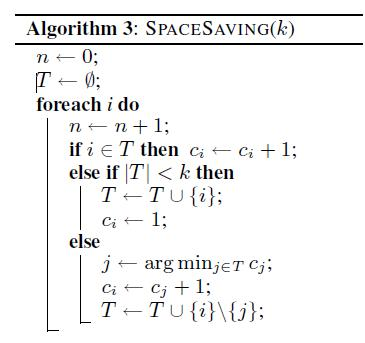
\includegraphics[width=12cm]{images/besoins/code_spaceSaving.jpg}
    \caption{Pseudo-code de l'algorithme SpaceSaving (Source : voir \cite{SpaceSaving2}) \label{fig:codeSpaceSaving}}
\end{figure}

\begin{figure}[H]
	\centering
        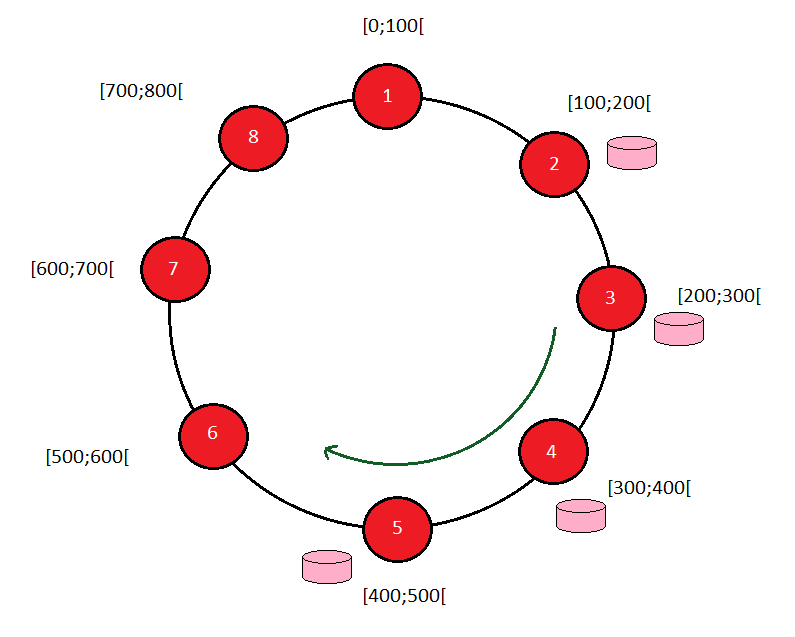
\includegraphics[width=12cm]{images/besoins/replication.png}
    \caption{Répartition des copies sur les noeuds dans une base de données distribuée \label{fig:replication}}
\end{figure}

%%%%%%%%%%% ARCHITECTURE %%%%%%%%%%%

\begin{figure}[p]
	\centering
		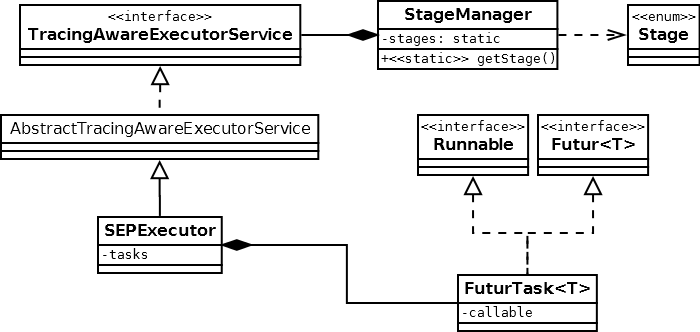
\includegraphics[width=15cm]{images/architecture/stages_diagram.png}
	\caption{Diagramme de classe simplifié de l'architecture SEDA dans Cassandra \label{fig:stages_diagram}}
\end{figure}

%%%%%%%%%% IMPLEMENTATION %%%%%%%%%%

\begin{figure}[H]
	\centering
        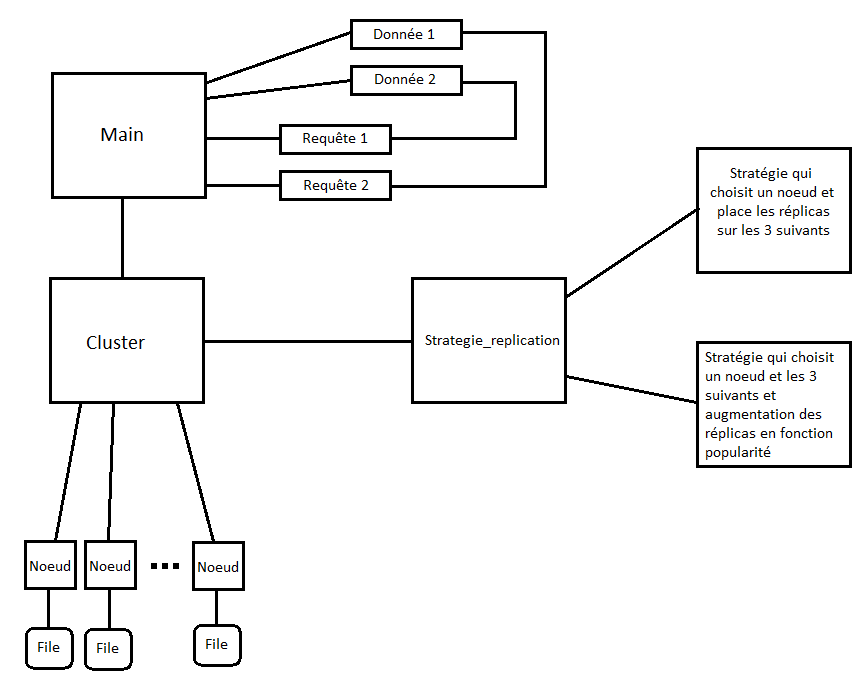
\includegraphics[width=12cm]{images/implementation/archiSimulateur.png}
    \caption{Architecture des objets du simulateur \label{fig:archisimulateur}}
\end{figure}

\begin{figure}[H]
	\centering
        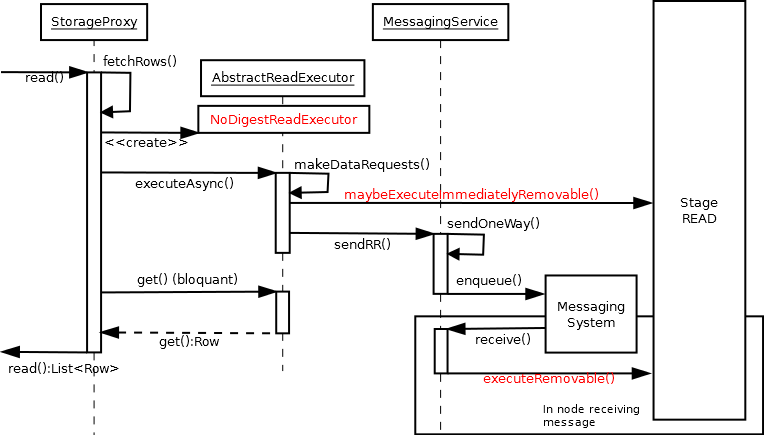
\includegraphics[width=12cm]{images/implementation/read_diagram_modified.png}
    \caption{Diagramme de séquence simplifié d'une requête de lecture dans Cassandra après modification \label{fig:read_diagram_modified}}
\end{figure}

\begin{figure}[p]
	\centering
		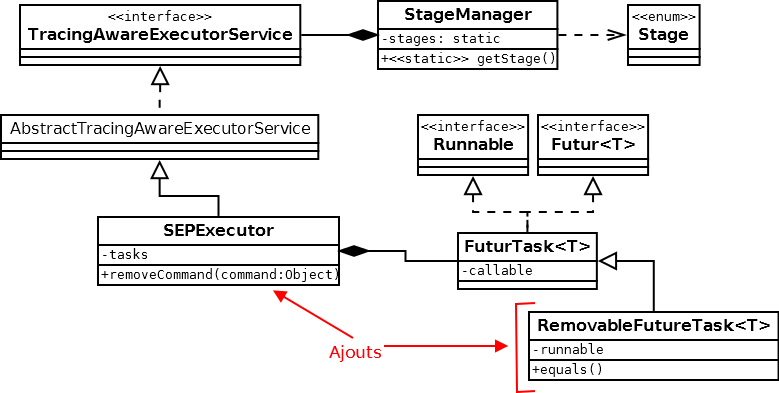
\includegraphics[width=15cm]{images/implementation/stages_diagram_modified.png}
	\caption{Diagramme de classe simplifié de l'architecture SEDA dans Cassandra après modification \label{fig:stages_diagram_modified}}
\end{figure}

%%%%%%%%%% TESTS %%%%%%%%%%

\begin{figure}[p]
	\centering
		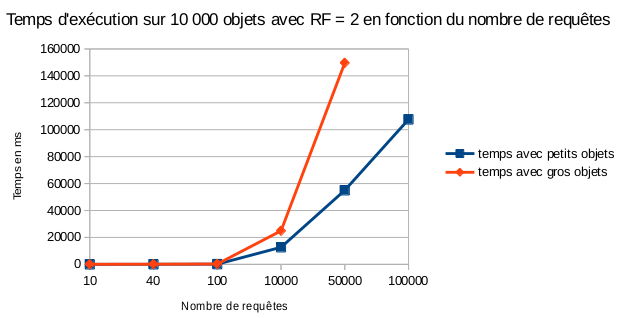
\includegraphics[width=15cm]{images/tests/PAF-TailleO-RF2.png}
	\caption{Comparatif des temps d'exécution de requêtes en fonction de leur nombre et de la taille des objets \label{fig:test_taille_RF2}}
\end{figure}

\begin{figure}[p]
	\centering
        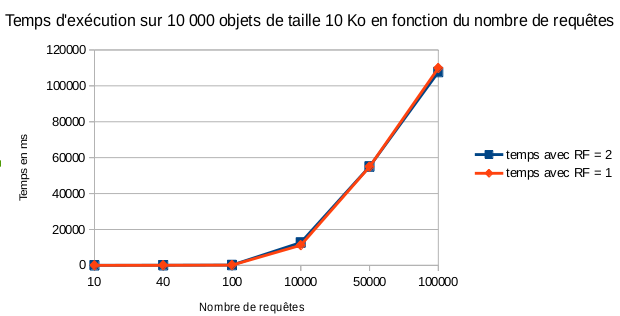
\includegraphics[width=15cm]{images/tests/PAF-RF-PO.png}
	\caption{Comparatif des temps d'exécution de requêtes en fonction du facteur de réplication et du nombre de requêtes sur des petits objets \label{fig:test_RF_PO}}
\end{figure}

\begin{figure}[p]
	\centering
		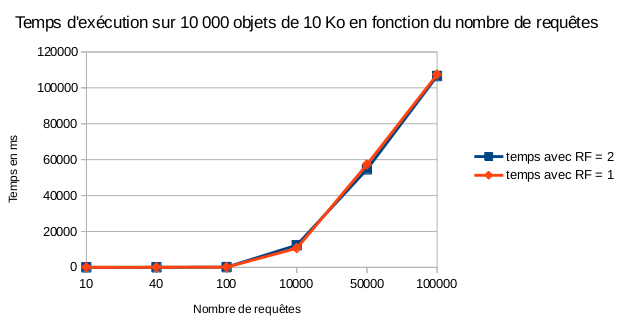
\includegraphics[width=15cm]{images/tests/cassandra_non_modif-RF-PO.png}
	\caption{Comparatif des temps d'exécution des requêtes en fonction du facteur de réplication et du nombre de requêtes sur des petits objets sur une base de Cassandra non modifiée \label{fig:test_cassandra_non_modif_RF_PO}}
\end{figure}

\end{document}
